\documentclass[twoside]{AiTeX}
\usepackage{flafter}


\title{Memoria DSI}
\author{Grupo 2}
\date{Noviembre 2023}
\begin{document}
%\datos{facultad}{universidad}{grado}{asignatura}{subtitulo}{autor}{curso}
\datos{Informática}{Universidad Complutense de Madrid}{Ingeniería informática}{Just Travel It}{Memoria de proyecto - Hito 6: Evaluación Heurística}{ \underline{\textbf{Grupo 2}} \\ Alejandro Barrachina Argudo \\
    Sergio Colet García\\
    Maria Esteban Benito \\
    Javier Gómez Arribas \\
    Leire Jiménez González \\
    Pablo Lavandeira Poyato \\
    Laura Martínez Tomás \\
    Guillermo Novillo Díaz \\
    Rodrigo Souto Santos \\
    Carlos Varela Sansano \\
    Daniel Yllana Santiago
}{2023-2024}
\portadaApuntes
\pagestyle{empty}
\tableofcontents
\pagestyle{empty}
\justify
\pagestyle{fancy}

\newpage

\newacronym{di}{D.I.}{Discapacidad Intelectual}


% \section*{Control de cambios} %
% \noindent\begin{tabularx}{\textwidth}{ |l|l|p{5cm}|X| }
%     \hline
%     \textbf{Versión} & \textbf{Fecha} & \textbf{Autores}     & \textbf{Descripción}                                                 \\
%     \hline
%     1.0              & 27/09/2023     & Alejandro Barrachina & Comienzo de la memoria\\
%     \hline
% \end{tabularx}

% \newpage

%\chapterA{Hito 2: Fase de Modelado}
\section{Listado de factoides}
El listado de factoides es el producto resultado de la fase de investigación. Para obtenerlo se ha extraído las principales características de las
diversas entrevistas, de todas las respuestas a los cuestionarios y del análisis de la competencia. Respecto a los obtenidos en el anterior hito,
hemos realizado una serie de cambios debido a la falta de respuestas a algunas de las variables que hemos identificado y a los problemas que se
han podido identificar durante la corrección de dichos factoides.


Tras la corrección del hito anterior y observando las necesidades del diseño de personas de este hito, vamos a realizar una serie de modificaciones
en la lista de factoides, reflejando los cambios que han sido realizados con la letra en cursiva. Cabe destacar que el usuario Alberto ha sido finalmente
descartado debido a que sus características no se encuadraban dentro de las propuestas en la hipótesis de usuarios. \\

\textbf{Factoides de Madi:}

\begin{itemize}
    \item Madi es secretaria de la FEDDI y lleva 16 años trabajando allí.
    \item Madi se encarga de organizar los viajes cuadrando horarios y comprando billetes.
    \item Madi compra billetes a través de Renfe, Air Europa o Iberia porque le sale más económico que en un comparador.
    \item Madi se encarga de los viajes de campeonatos internacionales que les recepciona, les recoge y les lleva al punto de encuentro.
    \item Madi ve que el problema principal para los deportistas es la dependencia de sus padres y entrenadores, el manejo de las aplicaciones y el internet y para algunos necesitan acompañante.
    \item Madi considera que necesitan acompañantes porque tienen problemas para orientarse y no se manejan bien.
    \item Para Madi las dificultades dependen mucho del grado de discapacidad.
    \item Madi no usa aplicaciones, sólo compra en páginas oficiales de la aerolínea.
    \item Madi utiliza la agencia de viajes Betravel para vuelos internacionales.
    \item Madi descarta Ryanair.
    \item Madi no utiliza comparadores porque ya tiene localizadas dos compañías y Renfe que ofrecen el servicio de acompañamiento de AENA.
    \item Madi tiene en cuenta el precio y la variedad de horarios para coger un billete.
    \item Madi no se fija en más facilidades, esos son los atletas.
    \item Madi considera que el comparador debe ser muy simple (lugar, destino y fecha).
    \item A Madi le parece importante que se pueda ver qué tipos de servicios de acompañantes ofrecen.
    \item \textit{En los campeonatos de España son los clubes los encargados del desplazamiento de los deportistas (ella no interviene)}.
\end{itemize}


\textbf{Factoides de Sofia:}

\begin{itemize}
    \item \textit{Sofía es estudiante, tiene 21 años y considera que tiene un buen manejo de la tecnología.}
    \item \textit{A Sofia le gusta viajar y considera que es uno de sus hobbies favoritos porque le gusta conocer nuevas culturas, vivir experiencias y explorar lugares desconocidos.}
    \item \textit{Sofía ha viajado por Europa, Estados Unidos y por el territorio nacional.}
    \item \textit{A Sofia le gustaría viajar más.}
    \item \textit{Sofía usa distintos métodos de transporte como coche, transporte público, avión, tren, bus y privado, este último rara vez.}
    \item \textit{Sofía prefiere usar autobuses solo cuando viaje distancias cortas o medias.}
    \item \textit{Sofía normalmente suele viajar con amigos y familiares por ocio.}
    \item \textit{Sofía no recuerda haber tenido ningún problema viajando, aunque admite que cuando viaja lo hace con la mente más abierta de lo que la tiene normalmente.}
    \item \textit{Sofía a veces organiza los viajes que hace y a veces no.}
    \item \textit{Sofía busca viajes económicos y que se adapten a sus necesidades.}
    \item \textit{Sofia utiliza varios comparadores de viajes a la hora de organizar un viaje para buscar las mejores ofertas. Por ejemplo: Kayak, Skyscanner, Trivago.}
    \item \textit{A Sofía le gustaría que los comparadores de viajes mostraran el precio final del billete, con los posibles extras incluidos, piensa que es un punto a mejorar.}
    \item \textit{Sofía prefiere usar aplicaciones web a aplicaciones móviles, y suele hacer estas gestiones desde el ordenador.}
    \item \textit{Sofía piensa que algunos comparadores son tediosos a la hora de usar ya que algunos tardan mucho en cargar o te redirigen a otra páginas.}
    \item \textit{Cuando Sofía ha tenido problemas con algún comparador ha optado por usar otro comparador que no tuviera esos problemas.}
    \item \textit{Sofía considera que con una interfaz sencilla y fácil de usar sería suficiente para un comparador.}
    \item \textit{Sofía considera que los comparadores de viajes son bastante accesibles, pero que quizás aclarar algunas cosas en las webs o los anuncios de spam en las webs pueden molestar a personas con discapacidad intelectual.}
    
\end{itemize}

\textbf{Factoides de Beatriz:}
\begin{itemize}
    \item Beatriz tiene 21 años.
    \item Beatriz se desenvuelve bien con las tecnologías y declara usarlas a diario.
    \item \textit{Beatriz viaja por ocio, para conocer nuevos lugares y culturas o visitar familiares.}
    \item Beatriz viaja una vez al año, sobre todo dentro de España, y fuera de España una vez cada dos años.
    \item \textit{A Beatriz le gustaría viajar más porque viaja poco para su gusto y salir de España más de una vez al año, los motivos por los que no puede hacerlo con más frecuencia es por su situación económica y el escaso tiempo que tiene de vacaciones.}
    \item Suele viajar en coche o en avión para distancias más largas.
    \item Beatriz suele viajar para visitar a familiares o por razones de ocio.
    \item Beatriz suele viajar acompañada (normalmente de sus familiares).
    \item Cuando viaja con su familia, organizan el viaje conjuntamente.
    \item \textit{Beatriz prioriza el precio del billete.}
    \item Cuando no viaja con su familia, Beatriz suele organizar los viajes que hace.
    \item Beatriz se fija sobretodo en el precio a la hora de tomar una decisión, por ejemplo, para comprar un vuelo.
    \item En su último viaje, Beatriz optó por usar una aplicación (eDreams) debido a que tenían un programa con prueba gratuita con el que sus vuelos le salieron más baratos.
    \item Beatriz prefiere los vuelos de ida tempranos y los de vuelta más tarde.
    \item A la hora de hacer la reserva, Beatriz cree que lo más tedioso son todas las pantallas que tienes que atravesar en las que te ofrecen todo tipo de servicios extra, alguno incluso ofreciéndose dos veces.
    \item A Beatriz también le gustaría que los comparadores pusieran un mensaje más claro en el caso de que ida y vuelta sean desde aeropuertos distintos.
    \item Google es su navegador favorito, principalmente porque lo lleva usando mucho tiempo y está acostumbrada, pero también debido a la conectividad con otros servicios en su móvil y porque considera que es lo mejor en cuanto a desarrollo web; también le gusta su estética.
    \item El comparador favorito de vuelos de Beatriz es el comparador de Google u otros.
    \item Beatriz considera que los comparadores de vuelos pueden no ser accesibles para personas que no tengan mucha soltura con las tecnologías.
    \item Beatriz considera que eDreams es muy estético, más que el comparador de Google o que otros.
    \item \textit{Para ella no es un problema sacrificar facilidades como el tipo y la cantidad de equipaje, la elección de asiento o los horarios de ida y vuelta para que el precio sea más barato}.
    \item \textit{Beatriz destaca también que al comprar en eDreams tuvo un problema con la aerolínea, lo que la llevó a tener que pasar un proceso poco accesible y con más cargos económicos.}
    \item \textit{Beatriz destaca que generalmente prefiere hacer estas reservas de viajes en el ordenador en vez de en el móvil.}
\end{itemize}


\textbf{Factoides del cuestionario:}

\begin{itemize}
    \item La mitad de los usuarios tienen entre 19 y 25 años y la otra mitad entre 26 y 65 años.
    \item La mayoría de los encuestados viven en la ciudad, pocos en pueblos.
    \item Dos tercios de los encuestados tienen un poder adquisitivo medio. Un tercio, bajo y muy pocos, alto.
    \item La mayoría de los encuestados les gusta viajar, pocos no.
    \item La mayoría de los encuestados le gusta viajar por conocer nuevos lugares y los pocos que no, es por la gente o por no parar de moverse.
    \item La mayoría de los encuestados viajan al menos una vez al año, el resto viajan al menos una vez al mes y muy poco no viajan.
    \item La mayoría de los encuestados le gustaría viajar más, el resto no.
    \item Todos los encuestados disfrutan cuando viajan.
    \item Los medios de transporte que usan los encuestados son coche propio, transporte público y aéreo.
    \item Los encuestados suelen viajar por ocio, pocos por trabajo.
    \item Las herramientas que más utilizan los encuestados son Trivago, Kayak y SkyScanner. Hay un tercio de los encuestados que no usan ninguna.
    \item Los comparadores de viajes (Trivago, Kayak, Rastreator, SkyScanner, Momondo) son de fácil uso.
    \item Un quinto de los encuestados tienen alguna discapacidad reconocida.
    \item Los encuestados con discapacidad la mayoría tienen discapacidad física y el resto es intelectual o mental.
    \item Los encuestados con discapacidad dos tercios necesitan adaptaciones para sus viajes como para sillas de ruedas.
    \item La mayoría de los encuestados con discapacidad a veces planifican y el resto o nunca o siempre.
    \item Un tercio de los encuestados con discapacidad encuentran dificultad en el proceso de búsqueda por la accesibilidad.
    \item La mayoría de los encuestados con discapacidad no les supone una dificultad buscar medio de transporte, hacer, comparar y ver las ventajas/desventajas de las rutas o comparar precios.
    \item La mitad de los encuestados con discapacidad no usan comparadores de viajes o similares.
    \item Los encuestados con discapacidad que han usado comparadores la mayoría ha desistido.
    \item Para los encuestados con discapacidad les parece complejo solicitar ayuda dentro de la aplicación de viajes.
    \item La inmensa mayoría de los encuestados sin discapacidad ha viajado en el último año.
    \item La mayoría de los encuestados sin discapacidad hace búsqueda de viaje.
    \item Dos tercio de los encuestados sin discapacidad han utilizado un comparador de viajes.
    \item El motivo principal de los encuestados sin discapacidad es ahorrar dinero. También está mayor oferta, facilidad de uso y ahorra tiempo.
    \item Los encuestados sin discapacidad no tienen problemas con los comparadores.
    \item A los encuestados sin discapacidad les supone una dificultad en el tema de la accesibilidad tener que hacer muchas operaciones para llegar a un objetivo.
    \item Los encuestados están de acuerdo en su mayoría de que está bien la accesibilidad salvo por la ausencia de ayudas al rellenar.
    \item La mayoría de los encuestados no ha echado en falta ninguna funcionalidad.
\end{itemize}


\textbf{Factoides del análisis de competencia}

\begin{itemize}
    \item Todas las aplicaciones ofrecen como mínimo poder buscar vuelos, algunas incluyen trenes y buses en las búsquedas
    \item Las funcionalidades buscadas en otras aplicaciones son búsqueda de medio de transporte, comparar precios para el mismo viaje, y comprar billetes
    \item Todas las aplicaciones tienen un sistema de opiniones y de valoración con estrellas
    \item Todas las páginas que ofrecen servicio de comparar transporte tienen buenos filtros de búsqueda
    \item Todas ofrecen como mínimo poder buscar vuelos, algunas incluyen trenes y buses en las búsquedas
    \item Casi todas ofrecen un sistema de seguros a la hora de comprar un medio de transporte
    \item Solo dos de las páginas estudiadas ofrecen opciones de ecologismo
    \item En los autobuses no es hasta el final de la reserva donde se puede designar que el cliente es una persona con discapacidad física
    \item En trenes al principio te deja marcar la casilla “Trenes con plaza H”, la cual es una plaza habilitada para personas con discapacidad física que necesitan una silla de ruedas 
    \item A la hora de realizar el pago puedes marcar la “tarjeta dorada”, la cual aplica un descuento para personas con discapacidad
    \item En los servicios de reserva de autobuses no es hasta el final de la reserva cuando se puede marcar que el cliente es una persona con discapacidad física.
    \item No todas ofrecen poder buscar con flexibilidad de fechas

\end{itemize}

%\chapterA{Introducción}

\textit{\app} ha surgido como proyecto debido a la necesidad de viajar que tienen las distintas personas con \gls{di}. Al
descubrir que muchas de éstas tienen problemas a la hora de reservar sus viajes con las páginas actualmente disponibles, decidimos crear un 
comparador de viajes que sean capaces de usar las personas con una limitación intelectual leve, o sus acompañantes en el caso de personas que
tengan una discapacidad mayor. 

Para lograr esto, vamos a empezar realizando una investigación sobre los usuarios potenciales y sus necesidades. Para esto realizaremos entrevistas
a distintos perfiles dentro de nuestras hipótesis de personas, para así poder diseñar la aplicación en referencia a sus experiencias y problemas a la hora
de viajar y/o buscar viajes. Junto a las entrevistas, también se realizará la observación de los usuarios en ámbitos de búsqueda de viajes, para poder hacer
una observación de éste. Además, para alcanzar una mayor demografía, haremos uso de cuestionarios, los cuáles nos permitirán también recibir información
en menor medida que en una entrevista, pero de más gente.

Después de la investigación, realizaremos un modelado de la aplicación, utilizando los resultados obtenidos para crear arquetipos de usuarios que
contengan información sobre los distintos objetivos que tendrían los perfiles potenciales. Gracias a esto, podríamos obtener usuarios que nos den
\textit{feedback} a la hora de avanzar con el diseño del sistema.

%\chapterA{Investigación}

\section{Introducción}

Para poder diseñar una aplicación correctamente, es muy importante realizar previamente una investigación para saber qué
es lo que realmente se necesita, y cuáles son los problemas de nuestro público objetivo. Hay muchas maneras de conseguir esto, pero en nuestro
caso, como desgraciadamente no disponemos del tiempo para poder usar todos los métodos, hemos realizado las siguientes.

\begin{itemize}
    \item \textbf{Entrevistas.} Es una de las partes más importantes de la investigación. Con estas entrevistas podremos sacar distintos tipos de usuarios y distintos casos de uso de los mismos. Aspiramos a tener 6 entrevistas.
    \item \textbf{Cuestionarios.} Con estos cuestionarios podemos conseguir una información más cerrada. Esta información puede ser interesante para comparar nuestra idea contra otras aplicaciones existentes en el mercado.
\end{itemize}



Pero antes de realizar esta labor, debemos saber reconocer cuál es el público objetivo de nuestra aplicación y
de qué manera podemos clasificar a los distintos perfiles dentro de los clientes potenciales. Para eso hemos realizado la
\textbf{Hipótesis de personas}.

\section{Hipótesis de personas}

En esta primera fase de investigación, el primer paso que vamos a seguir es la identificación de los posibles usuarios que vamos a tener
en nuestra aplicación. Nuestro principal objetivo, como hemos visto anteriormente, es ofrecer una herramienta que permita a las personas con
discapacidad intelectual tener la posibilidad de utilizar un comparador de viajes sin problemas. Los principales usuarios que hemos identificado
y los cuáles vamos a entrevistar en la posterior fase de entrevistas son los siguientes:

\begin{itemize}
    \item\textbf{Gente que viaja por negocio.} Gente que tiene que planear viajes por motivos laborales, bien sea para viajes nacionales o internacionales. Normalmente serán viajes individuales.
    \item\textbf{Gente que viaja por ocio.} Personas que viajan por turismo, normalmente en grupo.
    \item\textbf{Gente que viaja para ver a sus familiares.} Viajero recurrente.
\end{itemize}

Por otro lado, vamos a tener otros tipos de personas identificados, que no van a ser usuarios potenciales de nuestra aplicación pese a pertenecer a 
alguno de los anteriores grupos, por lo que en el momento que detectemos que se trata de una persona encuadrada en uno de estos tipos
vamos a finalizar la entrevista ó el cuestionario, ya que no vamos a poder extraer información de valor para nuestra aplicación.


\begin{itemize}
    \item {\textbf{Usuarios que prefieren viajar con todo planificado por una agencia.}} Se trata de aquellos usuarios que cada vez que quieren
        reservar un viaje no les importa realizar un gasto extra y prefieren que todo sea organizado por una agencia de viajes, sobre todo de cara a
        evitar la aparición de ciertos conflictos que pueden tener con otras aplicaciones de la competencia.
    \item {\textbf{Usuarios que no les guste viajar y no tengan la necesidad.}} Existen usuarios que no les gusta viajar y que además nunca se han visto
        (ni se van a ver en un futuro próximo), por lo que no nos van a resultar de interés para la aplicación, ya que el objetivo buscado son perfiles que
        hayan experimentado el proceso y puedan contarnos aquellos inconvenientes que han podido encontrarse a lo largo del proceso.
\end{itemize}
 
A modo de conclusión, los perfiles de usuario que tenemos, como se puede apreciar está influenciado por dos factores muy importantes: la necesidad (o ausencia de ella) para viajar; gente que viaja por motivos laborales o familiares y gente que viaja por placer y ocio, y

\section{Plan de investigación}

Para la investigación de \textit{\app} usaremos dos técnicas: entrevistas y cuestionarios. En las subsecciones \ref{subsec:entrevistas} y \ref{subsec:cuestionarios} hablaremos en detalle del número de instancias de cada técnica y de sus distintos objetivos en más detalle.

\subsection{Entrevistas} \label{subsec:entrevistas}

Las entrevistas serán el método principal de obtención de datos. Con las entrevistas podremos ver usuarios potenciales (y no potenciales) para la aplicación y podremos hacer preguntas con mayor detalle. Se fija el objetivo en 4 entrevistas.

Las tareas a realizar en las entrevistas son:
\begin{itemize}
    \item Crear un guion de entrevista con diversas preguntas para los distintos tipos de usuarios. Esta tarea se hizo el primer día tras conocer el proyecto y se encargaron en su mayoría Pablo y Javier, aunque todo el grupo estuvo implicado. Se le dedicó solo ese día.
    \item Reclutar usuarios de distintos clases para poder tener una imagen de cada tipo de usuario de la aplicación. De esta tarea se encargaron Sergio y Leire y se ha hecho durante todo el proyecto.
    \item Entrevistar a los usuarios. Esta tarea la han llevado a cavo Daniel, Javier y Sergio en su mayoría. Se ha hecho durante todo el proyecto y se le ha dedicado aproximadamente 5 horas.
    \item Resumir las entrevistas y sacar los datos más importantes de las mismas. Pablo y Laura han sido los encargados de este apartado, se han hecho justo después de cada entrevista. Se le ha dedicado otras 7 horas a este apartado.
    \item Realizar el mapa de empatía de cada usuario entrevistado. Guillermo se ha ocupado de los mapas de empatía de todas las entrevistas. Se le ha dedicado a esta tarea 4 horas.
\end{itemize}

\subsection{Cuestionarios} \label{subsec:cuestionarios}

Los cuestionarios son nuestro método de sacar una información más guiada, para corroborar hipótesis sobre el diseño que teníamos o para ver que se nos ha podido escapar. Hemos escogido unos 30 usuarios como meta.

Las tareas a realizar en los cuestionarios son:
\begin{itemize}
    \item Crear el cuestionario y dividirlo en secciones. Leire, Rodrigo y Alejandro se han encargado en su mayoría de la creación del cuestionario. Se le dedicó 3 horas a esta tarea y se realizó el día 2 de octubre.
    \item Distribuir el cuestionario por distintos medios para alcanzar una gran cantidad de usuarios. Tanto Alejandro como María se dedicaron a difundir estos cuestionarios por distintos grupos y correos. Se le dedicó media hora a esta tarea.
    \item Analizar los datos y sacar conclusiones. Alejandro se dedicó al análisis de datos de este cuestionario. Se dedicó una hora a esta tarea.
\end{itemize}

\subsection{Distribución de tareas}

Aunque hemos sido flexibles con la asignación de tareas, pondremos aquí un resumen de las tareas que ha hecho cada uno a parte de las mencionadas en el apartado anterior:

\begin{itemize}
    \item Análisis de la competencia. Daniel y Carlos se dedicaron a esta tarea. La tarea se realizó en en torno a 2 horas.
    \item Listado de factoides. María, Leire, Laura  y Rodrigo hicieron los distintos listados. Se dedicó un total de 4 horas en conjunto para hacerlo.
\end{itemize}

%%%%%%%%%%%%%%%%%%%%%%%%%%%%%%%%%%%%%%%%%%%%%%%%%%%%%%%%%%%%%%
\section{Entrevistas}
%%%%%%%%%%%%%%%%%%%%%%%%%%%%%%%%%%%%%%%%%%%%%%%%%%%%%%%%%%%%%%

Es la parte más importante de la investigación, ya que es de donde conseguiremos obtener más información. Consiste en realizar una serie de preguntas al usuario para
ver si encaja con los perfiles objetivo de nuestra aplicación, y en caso de hacerlo, obtener los datos necesarios para poder diseñarla. Gracias a esto podremos averiguar
cuáles son los problemas que tienen estas personas con los comparadores actuales y qué necesidades tendrían.

Tenemos distintos clientes que forman parte de nuestra hipótesis de personas, y ambos tienen necesidades distintas. Por tanto tendremos distintas preguntas
dependiendo del perfil al que nos enfrentemos.

Todas las entrevistas comenzarán presentándonos y preguntando el nombre al entrevistado. Tras eso, tendremos que pedir autorización para grabar imágenes, ya que las
grabaciones son necesarias para un posterior análisis y recabar así la mayor cantidad de información posible. Para que la entrevista sea más distendida, preguntaremos
si le podemos tutear. Tras esto, explicaremos nuestros objetivos con la aplicación y procederemos a realizar las preguntas.

\subsection{Preguntas a usuarios}

Al comienzo realizaremos el denominado como \textit{Screener}, es decir, una serie de preguntas para ver si el entrevistado es un cliente potencial. En caso de serlo,
podremos proceder con el resto de preguntas.

\begin{enumerate}
    \item {\textbf{?`Cuántos años tienes?}} sirve para encuadrar al usuario dentro de un marco de edad concreto y poder tratar con él en función de esto.
    \item {\textbf{?`Cómo de cómodo te sientes con la tecnología?}}
    \item {\textbf{?`Te gusta viajar? ?`Cuéntame por qué?}} es la pregunta que nos va a determinar si el usuario es potencial de la aplicación
                o si bien lo tenemos que descartar.
    \begin{enumerate}
        \item {\textit{Sí,}} usuario potencial. Tenemos que conocer ahora si le gusta viajar por ocio o bien lo tiene que hacer por negocios.
        \item {\textit{No,}} puede seguir estando dentro de la hipótesis de usuarios. En este caso las preguntas a hacer van a variar y van a
                        depender de la respuesta que nos de.
    \end{enumerate}
    \item {\textbf{?`Suele viajar?}} sirve para identificar si el usuario es apto, porque si no viaja no tiene sentido la aplicación.
    \item {\textbf{?`Le gustaría viajar más?}} sirve para saber si el usuario que no viaja tiene pensado viajar en un futuro y por tanto, considerarlo apto.
    \item {\textbf{?`Disfruta cuando viaja?}} sirve para entender al usuario que viaja y si va a usar la aplicación más o menos frecuente.
    \item {\textbf{?`Cuál es tu medio de transporte favorito y por qué?}} sirve para entender al usuario que viaja y si va a usar la aplicación más o menos frecuente.
    \item {\textbf{?`Qué tipo de viajes has hecho?}} sirve para entender al usuario que viaja y si va a usar la aplicación más o menos frecuente.
    \item {\textbf{?`Sueles viajar acompañado?}} tenemos que tener en cuenta si la persona con la que estamos tratando requiere de la
                ayuda de un acompañante que viaje con él para tenerlo en cuenta a la hora de desarrollar la aplicación y nos ayuda a conocer un poco al entrevistado.
    \item {\textbf{?`Por qué motivos suele viajar?}} sirve para identificar las motivaciones del usuario.
    \item {\textbf{?`Qué es lo que más le dificulta a la hora de viajar? ?`Hay algo más que le dificulte viajar?}} sirve para identificar molestias que tiene
                el usuario al planificar un viaje.
    \item {\textbf{?`Cuando vas a organizar un viaje, que es lo primero que haces?}}
    \item {\textbf{?`Te encargas tú de organizar el viaje?}} queremos conocer si el usuario tiene la iniciativa para organizar el viaje por sí solo o bien si
                recurre a profesionales como agencias de viajes o a terceras personas.
    \item{ \textbf{?`Cómo has organizado tus viajes?}}
    \begin{enumerate}
        \item {\textit{No:}} ?`No has pensado nunca en usar un comparador de viajes? queremos conocer si aunque el usuario recurra a agencias de viajes o
                        a otras personas para realizar el viaje usaría en algún momento nuestra aplicación.
        \item {\textit{Si:}} ?`Te has encontrado alguna dificultad en el proceso? está bien para finalizar el screener e introducir la siguiente parte.
    \end{enumerate}
    \item {\textbf{?`Te resulta más cómodo realizar estas búsquedas de viajes en una aplicación móvil o en una página web?}}
    \item {\textbf{?`Cuál es el factor clave que hace que se decante por esa opción en un viaje?}} sirve para saber sus prioridades.
    \item {\textbf{?`Influye el coste del viaje en su elección?}} sirve para saber más información.
    \item {\textbf{?`Cuál de las partes de una página tradicional de comparación de viajes te parece más tediosa?}} necesitamos conocer los problemas que
                puede encontrarse el usuario en las páginas tradicionales para tenerlo en cuenta y poder mejorarlo en nuestra aplicación. En caso de que
                la respuesta sea afirmativa, podemos preguntarle si existe alguna opción de ayuda dentro de la plataforma.
    \item {\textbf{En caso de que hayas tenido algún problema en estas páginas, ?`has podido solicitar ayuda de manera sencilla?}}
    \item {\textbf{?`Según tu opinión, ?`cómo debería ser la forma ideal en la que una aplicación muestre la información?}}
    \item {\textbf{?`Hay alguna función de las páginas tradicionales que consideres útil para tus necesidades?}}
    \item {\textbf{En caso de que hayas realizado alguna reserva de viaje, ?`has conocido y sido informado de forma clara de las condiciones
                        y políticas de cancelación del viaje?}}
    \item {\textbf{?`Te gustaría que estas páginas incluyesen más información sobre accesibilidad para viajeros con discapacidad?}}
    \item {\textbf{?`Podrías darme algún ejemplo de aplicación que te guste y uses a diario?}}: queremos poner al usuario en una situación
    en la que nos comente una aplicación que le guste para poder conocer los motivos que le llevan a ello.
    \item {\textbf{?`Consideras que es una aplicación accesible??`Por qué?}}: queremos conocer desde el punto de vista de la persona aquellos
    elementos y problemas que puede identificar dentro de la aplicación y que puedan suponer un problema.
    \item {\textbf{Acordarse de hacer el debriefing, para hacer un repaso de lo que ha dicho a ver si se acuerda de algo más.}}
    \item {\textbf{?`Se te ocurre algo más de lo que hemos hablado que podría ayudarnos?}}
\end{enumerate}

Al finalizar, le agradeceremos al entrevistado su tiempo y su participación en nuestro proyecto.


\subsection{Resúmenes de entrevistas}

\textbf{Entrevista 1 - Madi:} Entrevista hecha por videollamada\footnote{Enlace a la entrevista 1: \url{https://drive.google.com/file/d/1a6UrtghooaZqYAVYK9umbhKor8_vxPM1/view?usp=drive_link}}. Participantes: Daniel, Sergio, Leire y Guilermo, duración 19:21.

Resumen de entrevista, el mapa de empatía está representado en la figura \ref{fig:mapa_madi}.

\begin{itemize}
    \item FEDDI, está como secretaria pero se encarga de gestionar los viajes (horarios y logística) para llevar a los competidores.
    \item Lleva 16 años trabajando con ellos.
    \item Trabajo de campo: Prepara la mesa de premiación y eventos deportivos.
    \item Trabajo administrativo: Licencia, gestión de cara al público, pagar tasas…
    \item Las autonomías se gestionan del desplazamiento.
    \item Alrededor de 4 competiciones de natación y 5 de atletismo.
    \item Las personas con DI se manejan mal con el tema de aplicaciones, internet o necesitan acompañante.
    \item Pueden necesitar acompañante sobre todo por problemas de orientación.
    \item Busca en las páginas de las compañías que pueden salir baratos o con Renfe.
    \item Trabaja con una agencia (betravel).
    \item No usa un comparador porque ya tiene localizadas las compañías que funcionan correctamente con los destinos que frecuenta.
    \item Ryanair por ejemplo no lo usa porque puede retrasarse y te cobran por la maleta.
    \item Se fija en el precio, en los horarios y se asegura de que puedan ir los acompañantes.
    \item Aerolíneas:
    \begin{itemize}
        \item Nacional: AirEuropa, Iberia.
        \item Tren: Renfe.
    \end{itemize}
    \item Que la aplicación sea lo más simple posible para la gente con DI.
    \item Que sea más simple mirar los servicios que ofrece la compañía.
    \item Que exista una alerta para saber cuándo tienen que bajar del tren y así no se pierdan (esa es buena).
    \item Normalmente el servicio de acompañante tiene coste adicional. AENA lo da de forma gratuita, pero mucha gente no lo sabe y la gente paga el precio extra de la compañía (también está bien).
\end{itemize}


Transcripción resumen con marcas de tiempo:

\noindent\textbf{0:00 -- 0:08 $\rightarrow$} Presentación, se llama Madi y es la secretaria de la fundación. \\
\textbf{0:10 -- 0:18 $\rightarrow$} Madi da su consentimiento para grabar la entrevista. \\
\textbf{0:20 -- 1:00 $\rightarrow$} Daniel presenta el proyecto a Madi y nos cuenta que ella es la persona que se encarga de organizar los viajes para deportistas de alta competición. \\
\textbf{1:05 -- 2:00 $\rightarrow$} Daniel pregunta “Nos podrías comentar que es lo que haces tu en esta asociación y que es la asociación en concreto” Madi responde que la asociación FEDDI es la federación española de deportes para personas con discapacidad intelectual, ella como secretaria se encarga de si hay alguna concentración deportiva o algún evento internacional ella dice que no es como una agencia de viajes sino que se encarga de cuadrar horarios para tema logística de la organización y sacar los billetes a través de renfe o de alguna aerolínea o de derivar a una agencia de viajes. \\
\textbf{2:02 -- 2:14 $\rightarrow$} Daniel pregunta cuánto tiempo lleva trabajando en FEDDI, lleva 16 años trabajando con ellos. \\
\textbf{2:15 -- 4:36 $\rightarrow$} Daniel pregunta cómo es trabajar en esta federación y trabajar con personas con esta discapacidad en el dia a dia, Madi comenta que hay dos campos, el trabajo de campo y el trabajo administrativo, ella va a los 3 campeonatos más importantes, que tienen más participantes, en la práctica, ella lleva tema protocolo, entrega de medallas y pasando resultados deportivos, ella disfruta más el trabajo de campo por el trato con los deportistas. Comenta que en el trabajo administrativo lleva facturación, certificados, licencias y trabajo de cara al público. Ella se siente gratificada con el trabajo en el campo. \\
\textbf{4:40 -- 6:39 $\rightarrow$} Daniel le pregunta cómo es en el trabajo de campo, son los viajes y como es llevarlos a cabo con las personas con discapacidad, Madi comenta que en los campeonatos de españa, los clubes son los encargados del desplazamiento de los deportistas, ella interviene poco o nada. Ella se encarga más de los campeonatos internacionales, ella les recepciona, les recoge y les lleva al punto de encuentro, donde se reúne toda la selección. Comenta que hay bastantes campeonatos. \\
\textbf{6:45 -- 7:43 $\rightarrow$} Daniel pregunta que qué problemas tendrán los deportistas a la hora de organizar los viajes si tuviesen que organizarlos ellos, utilizando páginas como kayak, Madi responde que sus atletas el problema principal es la dependencia, que no se manejan bien con las aplicaciones y con internet, para desplazarse algunos necesitan un acompañante \\
\textbf{7:45 -- 8:30 $\rightarrow$} Daniel pregunta qué motivos piensa que necesitan un acompañante y qué problemas se pueden encontrar durante el viaje, Madi comenta que en el aeropuerto a la hora de hacer el check in en el aeropuerto y encontrar la puerta de embarque, tienen problemas para orientarse y no todos se manejan bien. \\
\textbf{8:31 -- 9:07 $\rightarrow$} Daniel pregunta qué problemas tienen con las tecnologías, Madi comenta que los atletas son dependientes de los padres y de los entrenadores, depende mucho del grado de discapacidad. \\
\textbf{9:09 -- 10:02 $\rightarrow$} Daniel le pregunta que qué utiliza a la hora de organizar los viajes, si utiliza ella de manera independiente o buscando páginas que ya existen. Ella no usa aplicaciones, se mete en la página web de la aerolínea donde sabe que los transportes le van a salir más económicos, Air Europa, Iberia o Renfe. En caso de tener que organizar o pedir presupuesto para vuelos internacionales, utilizan una agencia de viajes que se llama betravel. \\
\textbf{10:03 -- 11:39 $\rightarrow$} Daniel pregunta por qué busca directamente en una compañía en vez de usar un comparador donde salen distintas aerolíneas. Madi responde que porque en los lugares de origen de los deportistas ya tiene localizadas dos compañías que son las que funcionan ahí, y descarta aerolíneas como ryanair por el problema de si tienes que pagar la maleta aparte, y que tiene muchos problemas de retrasos, entonces no utiliza compañías de bajo coste que no te ofrecen asistencia.  Por lo que utilizan compañías que sí ofrecen el servicio de acompañamiento de aena. Comenta que con Renfe también utilizan este sistema de acompañamiento. \\
\textbf{11:40 -- 13:02 $\rightarrow$} Daniel pregunta por más factores que tiene en cuenta a la hora de coger el billete, como por ejemplo el precio. Madi comenta que sí, el precio es uno, y miran también variedad de horarios, ya que no todas las aerolíneas tienen amplio horario, comenta que siempre sale más económico buscarlo directamente en la página que utilizar un comparador de viajes. \\
\textbf{13:03 -- 14:00 $\rightarrow$} Daniel pregunta si se fijan si se fija en que la aerolínea ofrece más facilidades a la hora de viajar, comenta que no que solo compara con lo que ya ha comentado, que como suelen ser los mismos atletas ya tiene todo bastante mecanizado. \\
\textbf{14:03 -- 14:27 $\rightarrow$} Daniel pregunta qué compañías suelen utilizar, Madi responde que a nivel nacional Air Europa, Iberia y para trenes siempre en Renfe. \\
\textbf{14:37 -- 17:37 $\rightarrow$} Daniel comienza a hacer el debriefing y pregunta si hay algo más que quiera añadir de lo que ya ha comentado para ayudarnos a diseñar la aplicación accesible para personas con discapacidad intelectual. Madi comenta que debería ser muy simple, lugar, destino y fecha. Por ejemplo, comenta que estaría bien poder ver si la compañía ofrece servicio de asistencia, ya que a los padres les da miedo que vayan solos, los que van en tren que puedan tener una alerta para que sepan cuando se tiene que bajar. \\
\textbf{17:37 -- 18:55 $\rightarrow$} Daniel comenta que ninguna aplicación que ha visto ofrece el servicio de ver si se ofrece acompañante, Madi comenta que sería importante, ya que si solicitas este servicio normalmente tiene coste, pero aena ofrece ese servicio de manera gratuita y eso no aparece en ninguna página de aerolínea y por ello es desconocido. \\
\textbf{18:57 -- 19:21 $\rightarrow$} Daniel le pregunta si se le ocurre alguna cosa más que se le ocurra para ayudarnos y no se le ocurre nada así que Daniel le da las gracias y procede a terminar la llamada.


\textbf{Entrevista 2 - Sofia:} Entrevista hecha por videollamada\footnote{Enlace a la entrevista 1: \url{https://drive.google.com/file/d/1RUf5q8dvR_aoA2IjaGYwXAqlAuBsn4sl/view?usp=drive_link}}. Participantes: Guilermo y Laura, duración 21:13.

Resumen de entrevista, el mapa de empatía está representado en la figura \ref{fig:mapa_sofia}.



Transcripción resumen con marcas de tiempo:

\noindent\textbf{00:00 -- 00:17 $\rightarrow$} Guillermo se presenta y explica brevemente el proyecto que vamos a realizar a la entrevistada, Sofía. \\
\textbf{00:18 -- 00:32 $\rightarrow$} Sofía presta su consentimiento a la grabación de la entrevista. \\
\textbf{00:33 -- 02:36 $\rightarrow$} Presentación: Sofía es estudiante, tiene 21 años y considera que tiene un buen manejo de la tecnología. Le gusta mucho viajar y considera que es uno de sus hobbies favoritos porque le gusta conocer nuevas culturas, vivir experiencias y explorar lugares desconocidos. Ha viajado por Europa, Estados Unidos y por el territorio nacional. Aunque le gustaría viajar más y está siempre en búsqueda de uno. \\
\textbf{02:37 -- 07:09 $\rightarrow$} Preguntas generales: Sofía usa diversos métodos de transporte como el coche, el transporte público, el avión y el tren, así como transporte privado, en pocas ocasiones. Normalmente suele viajar con amigos y familia por ocio. \\
\textbf{07:10 -- 07:42 $\rightarrow$} Guillermo pregunta cuáles son las dificultades que ha podido encontrar a la hora de viajar, Sofía responde que al viajar pierdes la comodidad que puedes tener en casa, pero que no ha encontrado ningún problema en particular en sus viajes más allá de la aceptación cultural. \\
\textbf{07:43 -- 08:31 $\rightarrow$} Guillermo pregunta que a la hora de reservar un viaje qué es lo primero que hace y Sofía responde mirar precios y escoger el más económico y que se adapte a sus necesidades. \\
\textbf{08:32 -- 09:17 $\rightarrow$} Guillermo pregunta si es ella quien se encarga personalmente de buscar los viajes y Sofía responde que en ocasiones sí es ella la que lo realiza, pero cuando no lo hace participa en la decisión final. \\
\textbf{09:18 -- 10:15 $\rightarrow$} Guillermo pregunta si ha usado alguna vez algún comparador de viajes y Sofía le responde que ha usado múltiples comparadores, como Kayak, SkyScanner, y busca entre las distintas páginas las mejores ofertas. \\
\textbf{10:16 -- 11:45 $\rightarrow$} Guillermo pregunta si ha encontrado alguna dificultad en alguna de las páginas mencionadas anteriormente a la hora de realizar una reserva y Sofía le contesta que por lo general no y que el único punto negativo podría ser la subida de precios después de seleccionar una opción. Como solución a este problema se propone que se indique directamente el precio final a pagar. \\
\textbf{11:46 -- 12:00 $\rightarrow$} Guillermo pregunta si le resulta más fácil utilizar estas páginas en aplicación web o en aplicación móvil y Sofía responde que suele usar el ordenador para realizar las búsquedas. \\
\textbf{12:01 -- 13:10 $\rightarrow$} Sofía realiza varias búsquedas hasta encontrar la que se adecua a sus necesidades, prefiriendo una salida a una hora temprana sabiendo que va a ahorrar dinero. \\
\textbf{13:11 -- 14:24 $\rightarrow$} Respecto a la dificultad en el proceso de comparación, Sofía se ha encontrado con algunas páginas en las que la carga es muy lenta o pinchas en un enlace y te desvía a otra página. También considera que SkyScanner es una página que está bien implementada, fácil de usar y accesible. \\
\textbf{14:25 -- 15:14 $\rightarrow$} Cuando se ha encontrado con dificultades en la búsqueda, ha desistido de usar esa aplicación y ha optado por páginas alternativas. \\
\textbf{15:15 -- 15:33 $\rightarrow$} Sofía no requiere de necesidades particulares a la hora de visualizar la interfaz, es decir, con que se use una interfaz sencilla y fácil de usar sería suficiente. \\
\textbf{15:34 -- 16:40 $\rightarrow$} Guillermo pregunta si a la hora de reservar lee las condiciones y añadidos y Sofía le responde que normalmente sí y que en muchas ocasiones son las compañías las que realizan estos añadidos y no los propios comparadores. \\
\textbf{16:41 -- 17:53 $\rightarrow$} Guillermo pregunta si considera que estas aplicaciones son accesibles para personas con discapacidad y Sofía responde que depende del grado y tipo de discapacidad. \\
\textbf{17:54 -- 18:37 $\rightarrow$} Una de las aplicaciones que Sofía usa en su día a día es Whatsapp y considera que es accesible y fácil de usar. \\
\textbf{18:38 -- 21:00 $\rightarrow$} Guillermo comienza el debriefing y le pregunta si tiene algo más que añadir. \\
\textbf{21:01 -- 21:13 $\rightarrow$} Se procede a agradecer a la entrevistada y a la finalización de la entrevista.

\textbf{Entrevista 3 - Alberto:} Entrevista hecha por videollamada\footnote{Enlace a la entrevista 1: \url{https://drive.google.com/file/d/1qqx8KDAfCw4QjHHnp4rkoky2YeaGp_I6/view?usp=drive_link}}. Participantes: Leire y Sergio, duración 17:22.

Resumen de entrevista, el mapa de empatía está representado en la figura \ref{fig:mapa_sofia}.

\begin{itemize}
    \item \textbf{Alberto}
    \item \textbf{22 años}
    \item \textbf{Sin discapacidad}
    \item Se desenvuelve bien con la tecnología (informático)
    \item Usa Whatsapp, Twitter (actualidad), YouTube, Amazon
    \item Busca chollómetro para ver ofertas
    \item Le parecen fáciles de usar.
    \item Le gusta viajar para descubrir historias, paisajes y nuevas culturas
    \item Viaja por ocio solo
    \item Viaja una vez al mes más o menos (para ir al pueblo o a Cantabria)
    \item Le gustaría viajar más (quiere salir de España)
    \item Usa vehículo propio normalmente para viajar, hace 7 años que no va en avión
    \item No usa Uber, muy ocasionalmente usa el taxi, pero prefiere el transporte público.
    \item Hace poco fue a Burgos, pero en coche
    \item Suele viajar con su pareja
    \item No tiene muchas dificultades a la hora de viajar (se prepara un itinerario de antes)
    \item Antes iba a la aventura a viajar
    \item No le resulta difícil, sobre todo le resulta tediosa
    \item Cuando viaja le gusta ir buscando el itinerario que es lo mejor para ver
    \item Hacen la organización en conjunto.
    \item Prefieren conocer la península por ahora, por eso prefieren ir en coche, su búsqueda es sobre todo de hoteles.
    \item En alojamientos se basan en:
    \begin{itemize}
        \item Que les guste visualmente
        \item Buena localización, no quieren la periferia
        \item El precio
    \end{itemize}
    \item Al usar Booking, no le gusta que Booking le obligue a escoger fechas, preferiría que le dijese el más barato sin seleccionar fechas concretas.
    \item Tiene problemas en la sobrecarga de ofertas, prefiere ver unas pocas buenas.
    \item También le gustaría que se pudiesen destacar los puntos fuertes de cada alojamiento (no solo en precio, sino también en características como "más espacioso" o "más céntrico", etc.).
    \item Si hay muchas ofertas, es muy difícil hacer que alguna destaque.
\end{itemize}


Transcripción resumen con marcas de tiempo:

\section{Cuestionarios}

Los cuestionarios los hemos realizado finalmente con Formularios de \textit{Google}. El público objetivo de este cuestionario es gente de cualquier edad a la que le guste viajar. Este cuestionario se ha difundido por grupos de amigos, grupos de asociaciones de la facultad y a distintos familiares por \textit{Whatsapp}.

El público que buscamos para realizar este cuestionario eran personas que viajen al menos una vez al año y utilicen aplicaciones de comparación de algún tipo. Al ser un espectro bastante amplio podemos permitirnos difundir e formulario por un medio bastante amplio.

La finalidad de este cuestionario es el sacar información más concreta (frecuencia de viajes, aplicaciones usadas para estos) de un gran número de usuarios. El ``gran número'' de usuarios ha sido finalmente de 59 respuestas, de las cuales 6 son viajeros por trabajo y 52 viajantes por ocio, solo uno ha seleccionado la opción de ``otro''.

\subsection{Guión}
Las preguntas del cuestionario son las siguientes:
\begin{enumerate}
    \item\textbf{Edad.} Pregunta de screening para enmarcar el resto de la respuesta.
    \item\textbf{Género.} Una vez más, pregunta de screening.
    \item\textbf{Entorno en el que vive el encuestado.} Otra pregunta de screening para saber si el usuario vive en una ciudad o en el entorno rural.
    \item\textbf{Poder adquisitivo.} No entramos en muchos detalles, pero no es lo mismo la comparativa que puede hacer una persona con unos recursos bajos y otra con unos recursos mayores. (observación). Pregunta de screening.
    \item\textbf{Gusto por viajar.} Es importante el contexto de si te gusta o no viajar para poder entender tus frustraciones con los sistemas de comparación.
    \item\textbf{La parte buena (o la parte mala) de viajar.} Queremos conocer las partes que más frustran a los viajantes para ver si es algo que nuestra aplicación pueda solucionar.
    \item\textbf{Frecuencia de viaje.} La gente que más viaje será la que más compare (intuitivamente), así que es importante saber la frecuencia en la que viaja un encuestado para tener más perspectiva sobre su opinión.
    \item\textbf{Posibilidad de viajar más.} Queremos saber si nuestros usuarios quieren viajar más y hay algo que se lo impida.
    \item\textbf{Disfrute al viajar.} Parece similar a la  pregunta 5, pero a una persona puede no gustarle alguna parte del proceso del viaje y aun así disfrutar del resto del viaje.
    \item\textbf{Medios de transporte.} Al ser nuestra aplicación un comparador de viajes, necesitamos saber cuales son los medios de transporte más usados.
    \item\textbf{Motivos de viaje.} El viaje por ocio y el viaje por trabajo pueden presentar maneras muy distintas de como enfocar esa comparación y la forma en la que buscamos destino y medio de transporte.
    \item\textbf{Uso de herramientas y dificultad de las mismas.} Para hacer  una buena aplicación hay que conocer a la competencia, por ello queremos saber la opinión de nuestro público sobre otras aplicaciones populares.
    \item\textbf{Preguntas para gente con discapacidad:}
    \begin{enumerate}
        \item\textbf{Discapacidad, tipo (general) de discapacidad y adaptaciones.} Es importante para nosotros el saber que problemas pueden surgirle a alguien con algún tipo de discapacidad para tenerlo en cuenta en la aplicación.
    \item\textbf{Frecuencia en la que el encuestado organiza viajes.} Si el encuestado no organiza viajes es complicado que nos pueda dar mucho \textit{feedback} sobre aplicaciones de comparativa de viajes.
    \item\textbf{Dificultad en a la hora de buscar viajes y el tipo de dificultad.} No van a ser las mismas dificultades para gente con discapacidades físicas que para gente con discapacidades psíquicas.
    \item\textbf{Falta de funcionalidades en los buscadores tradicionales.} Queremos saber si los usuarios han echado en falta alguna característica en sus búsquedas.
    \end{enumerate}
    \item\textbf{Preguntas para gente sin discapacidades}
    \begin{enumerate}
        \item\textbf{Viajes en el último año.} Si un usuario ha viajado en el último año nos puede dar información bastante actualizada.
        \item\textbf{Organización del viaje.} Queremos saber si el usuario ha organizado algún viaje en el último año.
        \item\textbf{Uso de comparadores, agencias o ninguna de las dos opciones y sus principales motivos para ello.} Queremos saber si los usuarios usan comparadores y sus principales motivos para ello.
        \item\textbf{Problemas y accesibilidad de los comparadores.} Queremos saber la dificultad de los usuarios de la encuesta ante distintas características de los comparadores modernos.
        \item\textbf{Falta de funcionalidades.} Queremos saber si los usuarios han echado de menos alguna funcionalidad concreta en los comparadores tradicionales.
    \end{enumerate}
    
\end{enumerate}

Podemos ver que la mayor parte de la población viaja por ocio y se considera de clase media. Vemos también que la gente está bastante contenta con los comparadores actuales a los que solo le harían cambios menores o simplificaciones. La mayoría de usuarios viajan en coche propio o en transporte público (tren o bus). También vemos un uso prominente de comparadores de viajes para ahorrar tiempo y dinero.

\subsection{Enlaces}

Dejamos aquí los enlaces al cuestionario en bruto \footnote{Enlace al cuestionario: \url{https://drive.google.com/drive/folders/1btqEATkoGqjZbF4wd30f3foDVuh37EUI?usp=drive_link}} y a los resultados en una hoja de calculo \footnote{ Enlace a los resultados en bruto: \url{https://docs.google.com/spreadsheets/d/1pTHiN6l9IVTqoC7u9HCUusoRIATDoZgKK113m_7aHrQ/edit?usp=drive_link}}

\section{Analisis de la competencia}

Para identificar a la competencia primero debemos conocer cuales son las funcionalidades que va a tener nuestra aplicación para ver cuáles otras del mismo tipo se parecen. Las funcionalidades principales de nuestra aplicación serían:
\begin{itemize}
    \item Búsqueda de alojamiento.
    \item Búsqueda de medio de transporte.
    \item Comparar precios para el mismo viaje.
    \item Comprar billetes y alojamientos.
\end{itemize}

Hemos hecho una búsqueda intensiva de las aplicaciones que pueden tener similitudes con nuestra aplicación.

Vamos a diferenciar entre competencia total y competencia parcial. Las aplicaciones que definimos con competencia total, son aquellas que comparten casi en su totalidad las mismas funcionalidades que nuestra aplicación. Por otro lado, hemos definido como competencia parcial aquellas que comparten alguna funcionalidad similar a nuestra aplicación (solo búsqueda de medios de transporte o solo búsqueda de alojamiento).

\subsection{Competencia total}
\begin{itemize}
    \item\textbf{Kayak.} Es una aplicación que permite comparar alojamientos y medios de transporte, ofrece descripciones detalladas de los destinos con cosas que se pueden hacer en los lugares y cómo moverse por allí. Tiene un mapamundi con etiquetas de los sitios con los precios más baratos. Tiene un 1,8 de valoración sobre 5.
    \item\textbf{eDreams.} Es un comparador de viajes que ofrece búsqueda de transporte y alojamiento y además ofrece el paquete conjunto de las dos y también permite alquiler de coche. Tiene servicio prime para reducir el coste de los viajes.Tiene un 4 de valoración sobre 5.
    \item\textbf{Momondo.} Es un comparador de vuelos, alojamiento y ofrece viajes completos. Tiene una opción de alertas de precios. Tiene un 4 sobre 5 de valoración.
    \item\textbf{SkyScanner.} Es una aplicación para buscar transporte y alojamiento en un destino determinado en unas fechas determinadas ofrece las últimas ofertas y tiene una sección de recomendaciones. Tiene un 3,9 sobre 5 de valoración.
\end{itemize}

\subsection{Competencia parcial:}
\begin{itemize}
    \item\textbf{Trivago.} Es una aplicación para buscar y comparar alojamientos, tiene un sistema de opiniones para valorar el alojamiento, ofrece ofertas, tiene diferentes opciones para encontrar un alojamiento adecuado para las necesidades del usuario. Tiene un 2,8 de valoración sobre 5.
    \item\textbf{Iberia.} Es una aplicación de la aerolínea que permite comparar vuelos de Iberia o de sus filiales. también tiene Iberia plus con un sistema de puntos para obtener descuentos. Tiene un 3 de valoración sobre 5
    \item\textbf{Booking.} Esta web permite comparar y comprar sólo alojamiento, tiene colaboración con aerolíneas como Iberia para hacer descuentos. Tiene un 1,2 de valoración sobre 5.
\end{itemize}

\subsection{Dimensiones}

\textbf{Comparar transporte.} Realizar una comparación de múltiples medios de transporte en unas fechas. [Respuesta binaria, tabla \ref{table:comp-transporte}]
\begin{itemize}
    \item Vuelos
    \item Trenes
    \item Buses
    \item Flexibilidad de fechas 
    \item Filtros de búsqueda 
    \item Alquiler de coche 
\end{itemize}

\begin{table}[H]
    \centering
    \begin{tabular}{l|l|l|l|l|l|l|}
    \cline{2-7}
                                     & Vuelos & Trenes & Buses & Flexibilidad de fechas & Filtros de búsqueda & Alquiler de coche \\ \hline
    \multicolumn{1}{|l|}{Kayak}      & Si     & Si     & Si    & Si                     & Si                  & Si                \\ \hline
    \multicolumn{1}{|l|}{eDreams}    & Si     & Si     & No    & No                     & Si                  & Si                \\ \hline
    \multicolumn{1}{|l|}{Momondo}    & Si     & Si     & Si    & Si                     & Si                  & Si                \\ \hline
    \multicolumn{1}{|l|}{SkyScanner} & Si     & No     & No    & No                     & Si                  & Si                \\ \hline
    \multicolumn{1}{|l|}{Trivago}    & No     & No     & No    & No                     & No                  & No                \\ \hline
    \multicolumn{1}{|l|}{Iberia}     & Si     & No     & No    & Si                     & Si                  & No                \\ \hline
    \multicolumn{1}{|l|}{Booking}    & No     & No     & No    & No                     & No                  & No                \\ \hline
    \end{tabular}
    \caption{Tabla de posibilidad de comparación de transportes entre distintas plataformas}
    \label{table:comp-transporte}
\end{table}

\textbf{Comprar transporte.} Poder comprar un medio de transporte previamente comparado. [Respuesta binaria, tabla \ref{table:comprar-transporte}]

\begin{itemize}
    \item Sistema de puntos
    \item Suscripción prime 
    \item Ecologismo 
    \item Seguros
\end{itemize}

\begin{table}[H]
    \centering
    \begin{tabular}{l|l|l|l|l|}
    \cline{2-5}
                                     & Sistemas de puntos & Suscripción prime & Ecologismo & Seguros \\ \hline
    \multicolumn{1}{|l|}{Kayak}      & No                 & No                & No         & Si      \\ \hline
    \multicolumn{1}{|l|}{eDreams}    & Si                 & Si                & Si         & Si      \\ \hline
    \multicolumn{1}{|l|}{Momondo}    & No                 & No                & No         & Si      \\ \hline
    \multicolumn{1}{|l|}{SkyScanner} & Si                 & Si                & Si         & Si      \\ \hline
    \multicolumn{1}{|l|}{Trivago}    & No                 & No                & No         & No      \\ \hline
    \multicolumn{1}{|l|}{Iberia}     & Si                 & Si                & No         & Si      \\ \hline
    \multicolumn{1}{|l|}{Booking}    & No                 & No                & No         & No      \\ \hline
    \end{tabular}
    \caption{Tabla comparativa sobre distintas características de los sistemas de compra}
    \label{table:comprar-transporte}
    \end{table}

\textbf{Comparar alojamiento.} Realizar una comparación dde múltiples alojamientos en unas fechas. [Respuesta binaria, tabla \ref{table:comp-aloj}]

\begin{itemize}
    \item Opiniones 
    \item Valoración con estrellas 
    \item Filtros de búsqueda 
    \item Flexibilidad de fechas
\end{itemize}

\begin{table}[H]
    \centering
    \begin{tabular}{l|l|l|l|l|}
    \cline{2-5}
                                     & Opiniones & Valoración con estrellas & Filtros de búsqueda & Flexibilidad de fechas \\ \hline
    \multicolumn{1}{|l|}{Kayak}      & Si        & Si                       & Si                  & Si                     \\ \hline
    \multicolumn{1}{|l|}{eDreams}    & Si        & Si                       & Si                  & No                     \\ \hline
    \multicolumn{1}{|l|}{Momondo}    & Si        & Si                       & Si                  & Si                     \\ \hline
    \multicolumn{1}{|l|}{SkyScanner} & Si        & Si                       & Si                  & No                     \\ \hline
    \multicolumn{1}{|l|}{Trivago}    & Si        & Si                       & Si                  & No                     \\ \hline
    \multicolumn{1}{|l|}{Iberia}     & No        & No                       & No                  & No                     \\ \hline
    \multicolumn{1}{|l|}{Booking}    & Si        & Si                       & Si                  & Si                     \\ \hline
    \end{tabular}
    \caption{Tabla de funcionalidades de la comparación de viajes}
    \label{table:comp-aloj}
    \end{table}

\textbf{Comprar alojamiento.} Poder comprar un alojamiento previamente comparado. [Respuesta vinaria, tabla \ref{table:comprar-aloj}]

\begin{itemize}
    \item Sistema de puntos 
    \item Suscripción prime 
    \item Seguros
\end{itemize}

\begin{table}[H]
    \centering
    \begin{tabular}{l|l|l|l|}
    \cline{2-4}
                                     & Sistemas de puntos & Suscripción prime & Seguros \\ \hline
    \multicolumn{1}{|l|}{Kayak}      & No                 & No                & Si      \\ \hline
    \multicolumn{1}{|l|}{eDreams}    & No                 & Si                & Si      \\ \hline
    \multicolumn{1}{|l|}{Momondo}    & No                 & No                & Si      \\ \hline
    \multicolumn{1}{|l|}{SkyScanner} & Si                 & Si                & Si      \\ \hline
    \multicolumn{1}{|l|}{Trivago}    & No                 & No                & No      \\ \hline
    \multicolumn{1}{|l|}{Iberia}     & No                 & No                & No      \\ \hline
    \multicolumn{1}{|l|}{Booking}    & No                 & No                & No      \\ \hline
    \end{tabular}
    \caption{Tabla de comparación de las distintas funcionalidades de la compra / reserva de alojamientos}
    \label{table:comprar-aloj}
    \end{table}

\subsection{Recomendaciones de acción}

A raíz de los resultados obtenidos en las tablas vamos a sacar unas recomendaciones de acción que nos permitan saber qué nos quiere decir este estudio.

\begin{itemize}
    \item Todas las páginas que ofrecen servicio de comparar transporte tienen buenos filtros de búsqueda, debemos incluir un buen sistema de filtros.Todas ofrecen como mínimo poder buscar vuelos, algunas incluyen trenes y buses en las búsquedas, sería interesante incluir todas en nuestra aplicación. No todas ofrecen poder buscar con flexibilidad de fechas, así que vemos interesante incluir flexibilidad de fechas en nuestra aplicación. No todas ofrecen servicio de alquiler de coche, es interesante incluirlo en la aplicación.
    \item Muy pocas páginas de las estudiadas ofrecen un sistema de puntos y suscripción prime, puede ser interesante incluirlo en nuestra aplicación. Solo dos de las páginas estudiadas ofrecen opciones de ecologismo, valoramos que no es tan interesante incluirlo en nuestra aplicación. Casi todas ofrecen un sistema de seguros a la hora de comprar un medio de transporte, es interesante incluirlo.
    \item Todas las aplicaciones utilizan un sistema de opiniones y de valoración gráfica con estrellas a la hora de mostrar los alojamientos comparados. Es muy interesante incluir esto en nuestra aplicación. Así como filtros de búsqueda también tienen todas, es interesante incluir buenos filtros. No todas ofrecen flexibilidad de fechas a la hora de comparar los alojamientos, es interesante incluirlo en nuestra aplicación.
    \item Para comprar alojamientos solo una aplicación incluye un sistema de puntos para comparar alojamientos, puede no ser interesante incluir un sistema de puntos para los alojamientos. De las páginas estudiadas para comprar alojamiento, dos de ellas utilizan sistema de prime, es interesante incluirlo. De estas páginas para comprar alojamiento todas tienen un sistema de seguros, es muy interesante incluirlo.
\end{itemize}

\section{Mapas de empatía}

Los mapas de empatía son una técnica de investigación que permite conocer más en profundidad al usuario con el que se está tratando. Es una de las técnicas que se está comenzando a implementar actualmente en la mayoría de empresas y consta de una plantilla dividida por sectores en los que cada uno de ellos representa distintos “estímulos” que percibe el usuario. \\

En nuestro caso, hemos utilizado una de las plantillas proporcionadas por Creately, que sugiere que dividamos el espacio en 7 regiones. Cada una de estas regiones, como vamos a ver, se va a centrar en un aspecto distinto de la personalidad del usuario. Concretamente hemos elegido esta porque dentro de la oferta de plantillas de la aplicación era la más comprensible y completa, ya que se centraba en varios aspectos de la personalidad, como lo que hacen los usuarios o lo que sienten, motivo por el que optamos por trabajar a partir de ella. \\

Dentro de esta plantilla, como se ha visto, existen 7 regiones claramente diferenciadas y en la que se responde a una pregunta. Estas secciones son las siguientes:
\begin{enumerate}
    \item {\textbf{Who are we empathizing with? (?`Con quién estamos empatizando?)}}.  Describe brevemente al usuario y el papel que desempeña dentro de nuestra aplicación.
    \item {\textbf{What do they need to do? (?`Qué necesitan hacer?)}}. Explica los procesos que sigue el usuario para conseguir su objetivo y las herramientas que necesita para ello. A su vez también expone las razones por las que se considera que el usuario ha logrado su objetivo.
    \item {\textbf{What do they see? (?`Qué ven?)}}. Es una de las fases en las que hay que ponernos en la piel del usuario y en base a lo contado en las entrevistas / cuestionarios, intentar describir cómo ve los procesos y a las personas, identificando las dificultades que observa.
    \item {\textbf{What do they say? (?`Qué dicen?)}}. En este apartado vamos a extraer algunas de las principales frases que han sido obtenidas durante la fase de entrevistas y que nos van a poner en contexto de la situación del entrevistado.
    \item {\textbf{What do they do? (?`Qué hacen?)}}. Se trata de las acciones que realiza el usuario, deducidas en base a la información obtenida en las entrevistas.
    \item {\textbf{What do they hear? (?`Qué escuchan?)}}. En esta sección vamos a volver a ponernos en la piel del usuario para poder conocer aquellos estímulos auditivos que puede recibir (de familia y amigos por ejemplo).
    \item {\textbf{What do they think and feel? (?`Qué sienten o escuchan?)}}. Por último, vamos a centrarnos en los pensamientos y sentimientos del usuario, clasificándolos en función de lo perjudiciales o beneficiosos que van a resultar y aportando un pensamiento o sugerencia que hayan tenido de mejora en la entrevista.
\end{enumerate}

 Una vez seleccionada y descrita la plantilla definitiva con la que vamos a trabajar, comenzamos a completar los distintos mapas de los entrevistados. Dentro de cada una de ellas hemos ido añadiendo tarjetas con pequeñas piezas de información referente a la pregunta del correspondiente sector, completando poco a poco con pequeñas piezas de información. \\

Muchas de estas preguntas han sido respondidas con las respuestas proporcionadas por los usuarios en sus entrevistas, pero existen otras (como la número 3), en la que tendremos que servirnos de los datos obtenidos en las entrevistas o en los cuestionarios, poniéndonos en la piel del usuario intentando dar respuesta a estas cuestiones.
\subsection{Resultados}
\begin{figure}[H]
    \centering 
    \includegraphics[width=0.9\textwidth]{./mapas_empatia/Mapa de Empatía - Madi.pdf}
    \caption{Mapa de empatía de la entrevista 1}
    \label{fig:mapa_madi}
\end{figure}

\begin{figure}[H]
    \centering 
    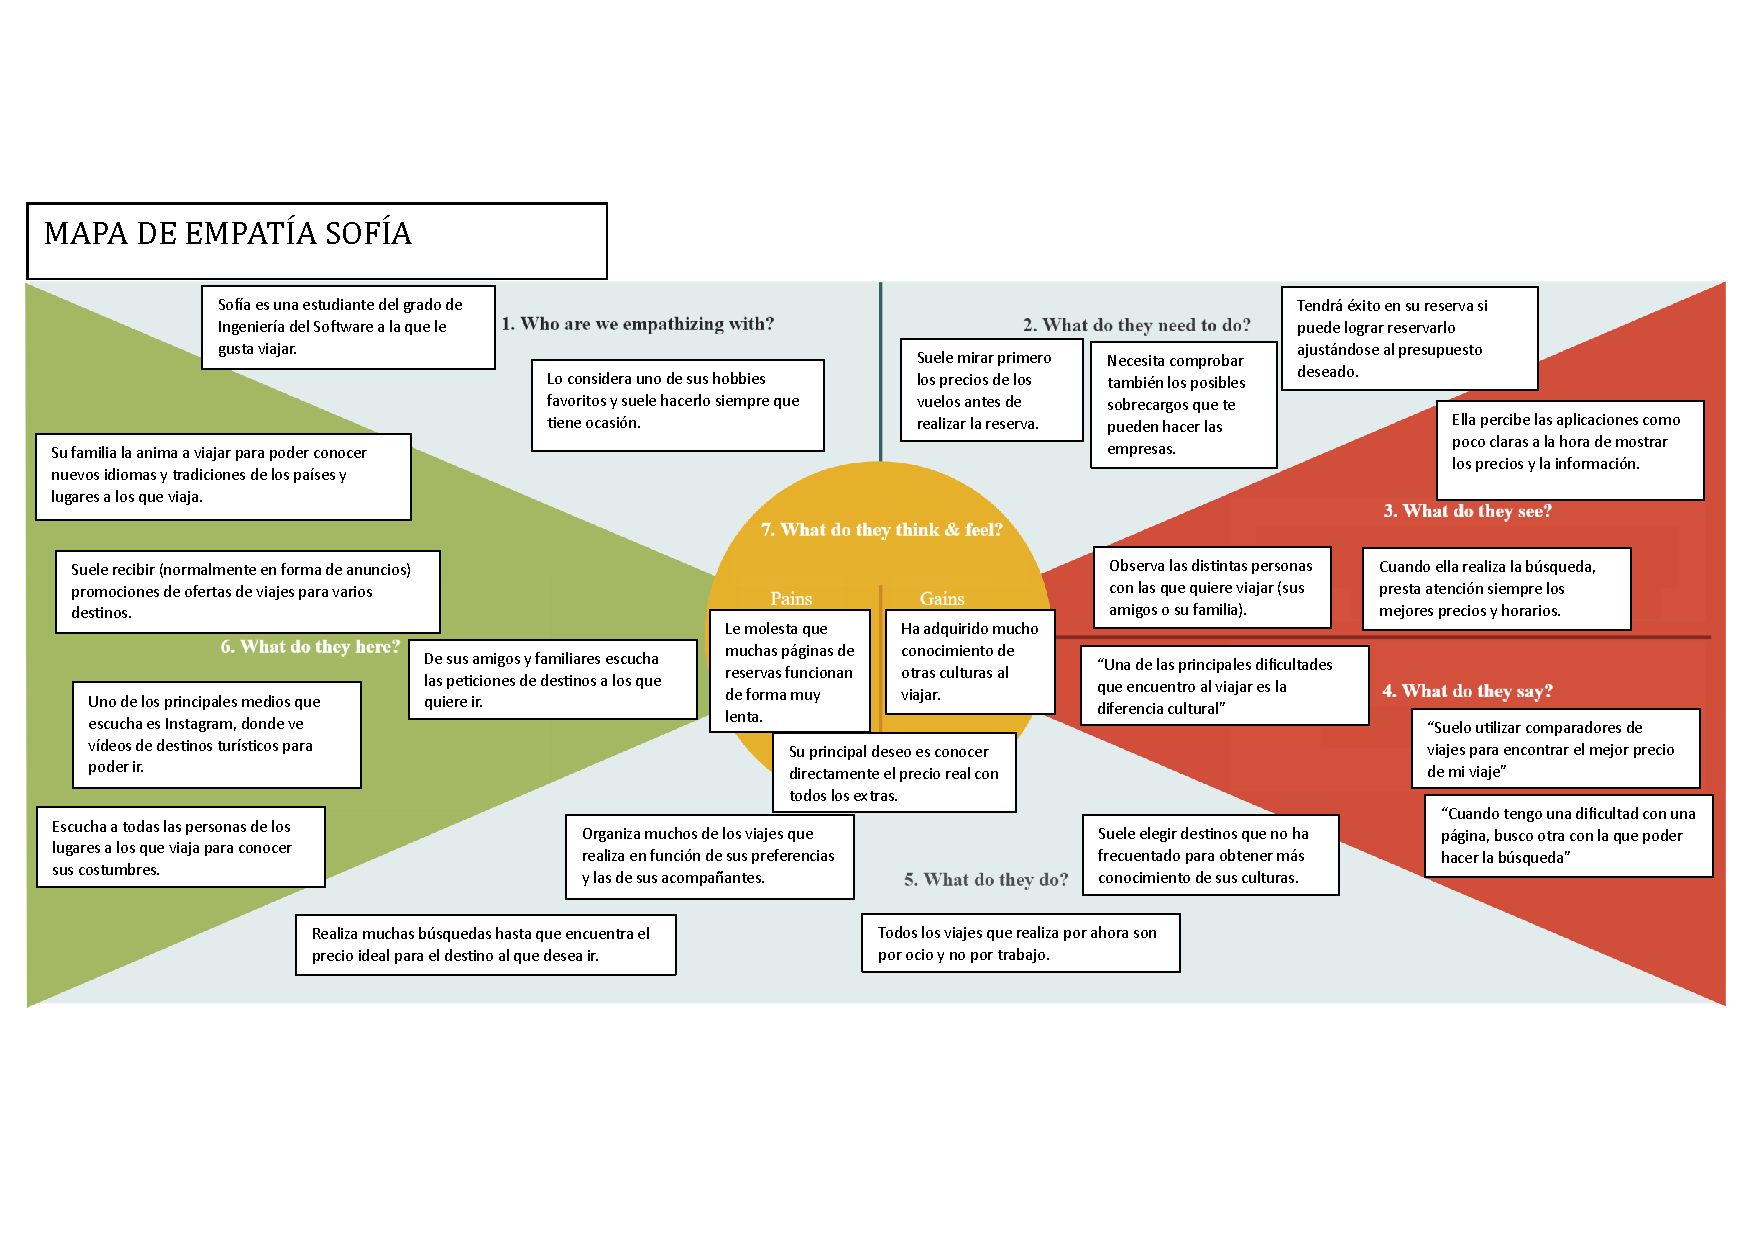
\includegraphics[width=0.9\textwidth]{./mapas_empatia/Mapa de Empatía - Sofía.pdf}
    \caption{Mapa de empatía de la entrevista 2}
    \label{fig:mapa_sofia}
\end{figure}

\begin{figure}[H]
    \centering 
    \includegraphics[width=0.9\textwidth]{./mapas_empatia/Mapa de Empatía - Alberto.pdf}
    \caption{Mapa de empatía de la entrevista 3}
    \label{fig:mapa_alberto}
\end{figure}

\begin{figure}[H]
    \centering 
    \includegraphics[width=0.9\textwidth]{./mapas_empatia/Mapa de Empatía - Beatriz.pdf}
    \caption{Mapa de empatía de la entrevista 1}
    \label{fig:mapa_bea}
\end{figure}

\section{Listado de factoides}

Tras realizar toda la investigación anterior, presentamos los factoides que hemos sacado de cada parte:

\textbf{Factoides de Madi:}

\begin{itemize}
    \item Madi es secretaria de la FEDDI y lleva 16 años trabajando allí.
    \item Madi se encarga de organizar los viajes cuadrando horarios y comprando billetes.
    \item Madi compra billetes a través de Renfe, Air Europa o Iberia porque le sale más económico que en un comparador.
    \item Madi se encarga de los viajes de campeonatos internacionales que les recepciona, les recoge y les lleva al punto de encuentro. Los nacionales los llevan los clubes.
    \item Madi ve que el problema principal para los deportistas es la dependencia de sus padres y entrenadores, el manejo de las aplicaciones y el internet y para algunos necesitan acompañante.
    \item Madi considera que necesitan acompañantes porque tienen problemas para orientarse y no se manejan bien.
    \item Para Madi las dificultades dependen mucho del grado de discapacidad.
    \item Madi no usa aplicaciones, sólo compra en páginas oficiales de la aerolínea.
    \item Madi utiliza la agencia de viajes Betravel para vuelos internacionales.
    \item Madi descarta Ryanair.
    \item Madi no utiliza comparadores porque ya tiene localizadas dos compañías y Renfe que ofrecen el servicio de acompañamiento de Aena.
    \item Madi tiene en cuenta el precio y la variedad de horarios para coger un billete.
    \item Madi no se fija en más facilidades, esos son los atletas.
    \item Madi considera que el comparador debe ser muy simple (lugar, destino y fecha).
    \item A Madi le parece importante que se pueda ver qué tipos de servicios de acompañantes ofrecen.
\end{itemize}


\textbf{Factoides de Sofia:}

\begin{itemize}
    \item Sofía tiene 21 años.
    \item A Sofía le gusta viajar y desde pequeña ha querido conocer las diferentes partes del mundo.
    \item Sofía viaja a menudo, tanto fuera como dentro de España.
    \item A Sofía le encantaría poder viajar más.
    \item Sofía usa tanto automóviles como coches, trenes y autobuses en sus viajes dependiendo del sitio al que viaje.
    \item Sofía prefiere usar autobuses solo cuando viaje distancias cortas o medias.
    \item Sofía ha hecho viajes de varios tipos. Desde intercambios lingüísticos a viajes familiares o con amigos, para conocer nuevas ciudades o relajarse.
    \item A Sofía le gusta ir alternando entre viajar sola, con familia o con amigos, disfruta de todas.
    \item Sofía no recuerda haber tenido ningún problema viajando, aunque admite que cuando viaja lo hace con la mente más abierta de lo que la tiene normalmente.
    \item Sofía a veces organiza los viajes que hace y a veces no.
    \item Sofía busca viajes económicamente accesibles.
    \item Sofía utiliza varios comparadores de viajes a la hora de organizar un viaje. Por ejemplo: Kayak, Skyscanner, Trivago.
    \item A Sofía le gustaría que los comparadores de viajes mostraran el precio final del billete, con los posibles extras incluidos, piensa que es un punto a mejorar.
    \item Sofía prefiere usar aplicaciones web a aplicaciones móviles, y suele hacer estas gestiones desde el ordenador.
    \item Sofía piensa que algunos comparadores son tediosos a la hora de usar, ya que algunos tardan mucho en cargar o te redirigen a otras páginas.
    \item Cuando le ha ocurrido esto, Sofía ha optado por usar otro comparador que no tuviera estos problemas.
    \item Como aportación, a Sofía le gustaría que los comparadores incluyeran el precio final de los billetes, desglosados con los diferentes conceptos.
    \item Sofía considera que los comparadores de viajes son bastante accesibles, pero que quizás aclarar algunas cosas en las webs o los anuncios de spam en las webs pueden molestar a personas con discapacidad intelectual.
    \item Sofía considera que Whatsapp es una aplicación accesible.
\end{itemize}


\textbf{Factoides de Alberto:}

\begin{itemize}
    \item Alberto tiene 22 años y es informático.
    \item Alberto no tiene discapacidad.
    \item Alberto se desenvuelve bien con las tecnologías y le parecen fáciles de usar.
    \item A Alberto le gusta viajar para descubrir historias, paisajes y nuevas culturas.
    \item Alberto viaja exclusivamente por ocio.
    \item Alberto viaja una vez al mes.
    \item A Alberto le gustaría viajar más, más adelante fuera de España.
    \item Alberto usa normalmente vehículo propio para viajar.
    \item Alberto hace 7 años que no viaja en avión.
    \item Alberto usa ocasionalmente taxis, pero prefiere el transporte público.
    \item Alberto descarta el uso de Uber.
    \item Alberto suele viajar con su pareja.
    \item Alberto prepara o busca un itinerario antes de viajar, incluso toma apuntes de paradas por si le falla el móvil o gps, le parece tedioso igualmente y se encarga con su pareja.
    \item Alberto sólo usa comparadores para alojamientos mirando lo visual que sea, la localización y el precio.
    \item Alberto usa Booking y le parece incómodo que le obliguen a poner fechas para ver el precio, prefiere ver el precio directamente.
    \item A Alberto le gusta ver pocas ofertas y más relevantes, y no ver muchas ofertas.
\end{itemize}


\textbf{Factoides de Beatriz:}

\textbf{Factoides del cuestionario:}

\begin{itemize}
    \item La mitad de los usuarios tienen entre 19 y 25 años y la otra mitad entre 26 y 65 años.
    \item La mayoría de los encuestados viven en la ciudad, pocos en pueblos.
    \item Dos tercios de los encuestados tienen un poder adquisitivo medio. Un tercio, bajo y muy pocos, alto.
    \item La mayoría de los encuestados les gusta viajar, pocos no.
    \item La mayoría de los encuestados le gusta viajar por conocer nuevos lugares y los pocos que no, es por la gente o por no parar de moverse.
    \item La mayoría de los encuestados viajan al menos una vez al año, el resto viajan al menos una vez al mes y muy poco no viajan.
    \item La mayoría de los encuestados le gustaría viajar más, el resto no.
    \item Todos los encuestados disfrutan cuando viajan.
    \item Los medios de transporte que usan los encuestados son coche propio, transporte público y aéreo.
    \item Los encuestados suelen viajar por ocio, pocos por trabajo.
    \item Las herramientas que más utilizan los encuestados son Trivago, Kayak y SkyScanner. Hay un tercio de los encuestados que no usan ninguna.
    \item Los comparadores de viajes (Trivago, Kayak, Rastreator, SkyScanner, Momondo) son de fácil uso.
    \item Un quinto de los encuestados tienen alguna discapacidad reconocida.
    \item Los encuestados con discapacidad la mayoría tienen discapacidad física y el resto es intelectual o mental.
    \item Los encuestados con discapacidad dos tercios necesitan adaptaciones para sus viajes como para sillas de ruedas.
    \item La mayoría de los encuestados con discapacidad a veces planifican y el resto o nunca o siempre.
    \item Un tercio de los encuestados con discapacidad encuentran dificultad en el proceso de búsqueda por la accesibilidad.
    \item La mayoría de los encuestados con discapacidad no les supone una dificultad buscar medio de transporte, hacer, comparar y ver las ventajas/desventajas de las rutas o comparar precios.
    \item La mitad de los encuestados con discapacidad no usan comparadores de viajes o similares.
    \item Los encuestados con discapacidad que han usado comparadores la mayoría ha desistido.
    \item Para los encuestados con discapacidad les parece complejo solicitar ayuda dentro de la aplicación de viajes.
    \item La inmensa mayoría de los encuestados sin discapacidad ha viajado en el último año.
    \item La mayoría de los encuestados sin discapacidad hace búsqueda de viaje.
    \item Dos tercio de los encuestados sin discapacidad han utilizado un comparador de viajes.
    \item El motivo principal de los encuestados sin discapacidad es ahorrar dinero. También está mayor oferta, facilidad de uso y ahorra tiempo.
    \item Los encuestados sin discapacidad no tienen problemas con los comparadores.
    \item A los encuestados sin discapacidad les supone una dificultad en el tema de la accesibilidad tener que hacer muchas operaciones para llegar a un objetivo.
    \item Los encuestados están de acuerdo en su mayoría de que está bien la accesibilidad salvo por la ausencia de ayudas al rellenar.
    \item La mayoría de los encuestados no ha echado en falta ninguna funcionalidad.
\end{itemize}


\textbf{Factoides del análisis de competencia}

%\chapterA{Hito 3 - Requisitos}

\section{Personas}

Tendremos dos personas, Marta (ver foto \ref{fig:fotoMarta}) e Isabel (ver foto \ref{fig:fotoIsaP}) \\

Para configurar estas personas, hemos utilizado un formato en el que vamos a dar en primer lugar la información general de la persona 
(edad, sexo, estudios y gustos). Posteriormente vamos a poner una foto de la persona (generada por una inteligencia artificial) y por último 
una descripción más elaborada de la persona, conteniendo la gran mayoría de los factoides e ideas expresadas en los esqueletos de las personas. 
Para poder destacar estas ideas, las hemos puesto en cursiva. \\

La estructura que van a tener las distintas personas va a seguir la siguiente configuración (ver figura \ref{fig:estructura-personas}) con los contenidos que hemos mecionado anteriormente.
\begin{figure}[h]
    \centering
    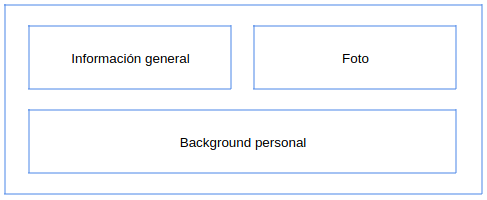
\includegraphics[width=0.5\textwidth]{Imagenes/Personas/Plantilla personas.png}
    \caption{Estructura de las personas}
    \label{fig:estructura-personas}
\end{figure}

\subsubsection{Marta González Torres}

\begin{minipage}{0.4\textwidth}
    \textbf{Información general} \\

    Edad: \textit{23 años} \\
    Sexo: Mujer \\
    Estudios: Ingeniería de Telecomunicaciones \\
    Gustos: Escuchar música e ir a conciertos cuando puede \\
\end{minipage}
\hfill
\begin{minipage}{0.4\textwidth}
    \centering
    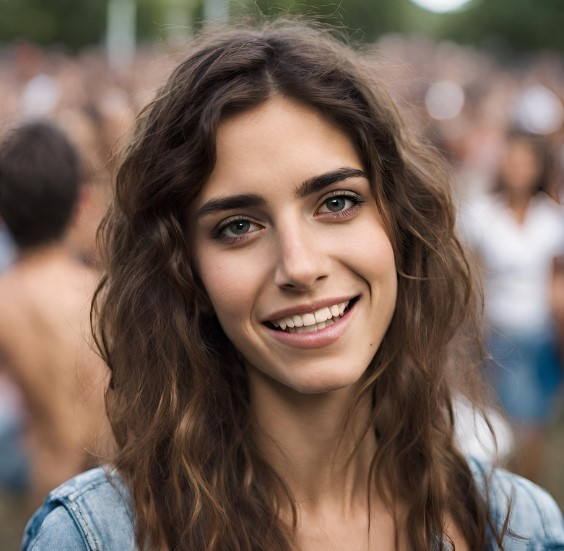
\includegraphics[width=0.5\textwidth]{Imagenes/Personas/Marta.jpg}
    \label{fig:fotoMarta}
    \captionof{figure}{Fotografía de Marta}
\end{minipage}

\textbf{Background personal} \\

Marta no puede salir de su casa sin los auriculares. Para ella la música es una gran parte
de su vida, y todas las mañanas, en la parada del bus, \textit{se prepara un playlist personalizada
en Spotify} para el itinerario hasta la Universidad. \textit{Vive en Fuenlabrada}, por lo que tiene
una ruta de una hora hasta que llega a Madrid, \textit{donde va a clase en la UCM}. \\ 

A Marta sobre todo le gusta la música italiana, ya que en el 2020 se fue de Erasmus a Turín y se
enamoró tanto de su cultura como de su música. Su cantante favorita es Francesca Michielin, así que
cuando hace gira intenta ir a algún concierto suyo en una \textit{ciudad italiana en la que no haya
estado}. De esta manera, puede conocer más la cultura italiana que tanto le gusta y sus diferenciados
a lo largo del país. \\

Se da la casualidad de que a su hermano Julián también le gusta mucho Francesca, así que en varias
ocasiones \textit{han ido ellos de viaje junto a sus padres} Carlos y Elena, los cuáles se van a
cenar juntos mientras sus hijos están en el concierto. \textit{Esto no lo hacen muy a menudo} debido
a que solo van cuando hay un concierto en alguna ciudad que les resulte interesante a toda la familia.
Normalmente se encarga ella de hacer la reserva tanto de los vuelos, \textit{para lo que usa
SkyScanner, como del alojamiento, utilizando AirBnB en este caso}. Esto se le hace a veces complicado
ya que quieren ir a varios sitios y tiene que cuadrar los horarios de todo. Por este motivo prefiere usar la 
aplicación web de las compañías, ya que así puede tener varias pestañas abiertas en las que visualiza toda
la información a la vez. \\

Con respecto al tema universitario, a Marta se le está haciendo cuesta arriba. Se metió inicialmente
en telecomunicaciones porque \textit{se le daban bien las matemáticas y la tecnología}, pero la
carrera no fue lo esperado. A pesar de las dificultades, la carrera le gusta y querría terminarla,
ya que este será en principio su último año. Pero estos problemas la agobian bastante, y para
distraerse le gusta mucho \textit{ir a festivales de música por España}. Suele ir todos los años
al festival Starlite, pues Pablo, el novio de su hermano y con el que mantiene muy buena relación,
es de Marbella, y se puede quedar algunos días en la playa aprovechando el viaje. Pero a pesar de
que no tiene que pagar gastos de alojamiento, el evento musical es bastante caro (ya que va varios
días), por lo que \textit{intenta ahorrar lo máximo posible en el viaje}. Para eso usa comparadores
de viaje como Omio, además de revisar las páginas de aerolíneas como \textit{RyanAir}, ya que a veces son
incluso más baratas que un vuelo o un tren.

\subsubsection{Isabel García Rodríguez}
\begin{minipage}{0.4\textwidth}
    \textbf{Información general} \\

    Edad: \textit{30 años} \\
    Sexo: Mujer \\
    Estudios: Psicología \\
    Gustos: Pintura y participar en grupos de apoyo para personas con discapacidad. \\
\end{minipage}
\hfill
\begin{minipage}{0.4\textwidth}
    \centering
    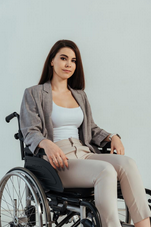
\includegraphics[width=0.5\textwidth]{Imagenes/Personas/Isabel.png}
    \label{fig:fotoIsaP}
    \captionof{figure}{Fotografía de Isabel}
\end{minipage}

\textbf{Background personal} \\

Isabel es una psicóloga comprometida con la mejora de la calidad de vida de las personas con discapacidad. \textit{Tiene una 
discapacidad física desde su nacimiento} que afecta su movilidad y requiere el uso de una silla de ruedas. Actualmente
\textit{vive en una pequeña urbanización a las afueras de Barcelona}. \\

Su familia vive en un pequeño pueblo de Huesca, por lo que \textit{siempre que puede se desplaza para verlos}. Muchas veces 
tiene el problema de la falta de autobuses que conectan con el pueblo, por lo que \textit{utiliza Omio, que realiza el trayecto
por ella, indicándole los transbordos que tiene que realizar y facilitándole la ayuda que necesita en todo momento}. \\

Ha asistido a varios cursos y conferencias relacionados con la psicología y la discapacidad, lo que la ha llevado a 
\textit{planear viajes a diferentes ciudades para participar en eventos}. Utiliza comparadores de viaje para encontrar opciones 
que se adapten a sus necesidades específicas, como hoteles con habitaciones adaptadas y \textit{vuelos con asistencia en el 
aeropuerto}. \textit{Algunos de los comparadores que usa no tienen opción de solicitar ayuda en caso de que tengas dudas, por lo que si
tiene algún problema no puede contactar con nadie}. Antes de realizar la reserva, ella sabe las distintas compañías y empresas que te lo suelen proporcionar. \\

Aparte de su trabajo, Isabel es una apasionada de la pintura y trata de visitar galerías y estudios de artistas en cada 
destino que visita. Isabel también es miembro activo de grupos de apoyo para personas con discapacidad en su ciudad. \textit{Allí 
es donde comparte experiencias y ofrece apoyo a otros miembros, por ejemplo a los jóvenes con discapacidad, para fomentar 
su independencia y autoestima}. Viaja a menudo con su mejor amiga, Carmen, quien la ha apoyado en su viaje de empoderamiento 
y ha aprendido mucho sobre la discapacidad en el proceso también.

\subsection{Tipos de personas}
\begin{itemize}
    \item \textbf{Persona Primaria} - \textit{Marta González Torres (Viajero que usa comparadores de viajes)} $\rightarrow$ Representa al tipo de usuario consumidor de comparadores de viajes. Se tratan de usuarios que utilizan activamente las funcionalidades de los comparadores con el objetivo de ahorrar lo máximo posible en los transportes para sus viajes.
    \item \textbf{Persona Secundaria} - \textit{Isabel García Rodríguez (Viajero con discapacidad)} $\rightarrow$ Representa al tipo de usuario consumidor o no consumidor de comparadores de viajes que tienen una necesidad añadida o distinta al resto de usuarios. 
    Generalmente usuarios que aparte de la interfaz ya creada necesitaran de una pequeña adaptación visual o sensorial para poder sacar el máximo provecho a la aplicación. En el caso de Isabel necesitaría un apoyo extra debido a su discapacidad que presenta, ya que sus viajes esterían mucho más condicionados que los de Marta.
\end{itemize}

\section{Fase de Requisitos}
La siguiente fase que vamos a abordar en el proceso de Diseño Guiado por Objetivos (DGO) es la fase de requisitos. En esta fase, vamos a tomar como punto de partida las personas que generamos en el hito anterior. A partir de ellas, vamos a estudiarlas en profundidad para obtener soluciones de diseño que satisfagan sus necesidades. Para ello, el proceso que vamos a seguir para definir los requisitos de las personas va a ser el método propuesto por Cooper, que consta de cuatro etapas diferenciadas:
\begin{enumerate}
	\item \textbf{Enunciado de problemas y visiones} $\rightarrow$ vamos a estudiar en detalle la información contenida en las personas que hemos desarrollado, 
    de modo que a partir de ellas vamos a intentar identificar los problemas que tienen y aportar cómo vamos a plantear una solución para este problema.
    \item \textbf{Identificación de las expectativas de las personas} $\rightarrow$ en esta segunda etapa, se va a tomar como punto de partida las distintas personas
    y para cada una de ellas vamos a analizar sus pensamientos, deseos, comportamientos y conocimientos que la persona va a tener en el ámbito de la aplicación.
    \item \textbf{Construcción de los escenarios de contexto} $\rightarrow$ en este apartado, van a redactarse para cada una de las personas que se han identificado, un
    escenario de contexto, que ponga en situación a la persona, persiguiendo un objetivo y describiendo el proceso que sigue para ello.
    \item \textbf{Identificaión de requisitos} $\rightarrow$ se trata de la fase final de este hito. En este apartado van a aparecer fusionadas todos los requisitos de
    las distintas personas que hemos ejemplificado, determinando cuáles son las necesidades que tienen y cuál va a ser el medio que necesitan para que puedan ser
    satisfechas estas necesidades en nuestra aplicación.
\end{enumerate}

\section{Planificación del hito}
Para poder planificar este hito correctamente, hemos identificado en una Hoja de cálculo (ver figura \ref{fig:planif-hito3}) las distintas tareas que tenemos que 
realizar, junto al intervalo de fechas en el que se encuentra prevista su realización y el / los responsables de dicha tarea.
\begin{figure}[H]
    \centering 
    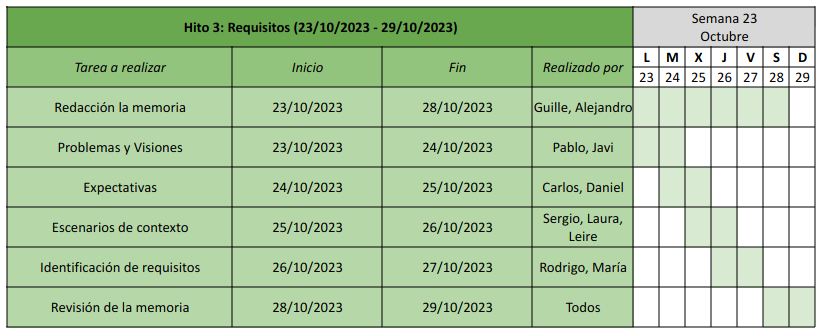
\includegraphics[width=0.5\textwidth]{./Imagenes/Planificaciones/Planif-hito3.png}
    \caption{Planificación Hito 3}
    \label{fig:planif-hito3}
\end{figure}

\section{Enunciado de problemas y visiones}

\begin{problema}

    Las personas que utilizan comparadores de viajes, en su gran mayoría, no tienen un gran poder adquisitivo: ``Suele ir todos los años al festival Starlite, pues Pablo, el novio de su hermano y con el que mantiene muy buena relación, es de Marbella, y se puede quedar algunos días en la playa aprovechando el viaje. Pero a pesar de que no tiene que pagar gastos de alojamiento, el evento musical es bastante caro (ya que va varios días), por lo que intenta ahorrar lo máximo posible en el viaje. Para eso usa comparadores de viaje como Omio.''

    {\centering\begin{vision}
    Nuestra aplicación ofrecerá los viajes más baratos al comienzo de la búsqueda cuando el usuario lo solicite dentro de unas fechas y una serie de filtros, además, podrá modificar filtrar la búsqueda ordenando las opciones como él prefiera.
    \end{vision}}
    \end{problema}
    
    \begin{problema}

    Las aplicaciones móviles son menos intuitivas que las webs: ``Para hacer este tipo de reservas prefiere utilizar aplicaciones web en vez de aplicaciones móviles ya que son más intuitivas.''

    {\centering\begin{vision}
    Nuestra app va a ofrecer la información justa y necesaria, sacaremos una versión ``Alpha'' para poder aprender de ella y mejorarla a través del uso.
    \end{vision}}
    \end{problema}

    \begin{problema}

        Numerosas aplicaciones web o móviles no están adaptadas a las diferentes discapacidades que puedan poseer los usuarios: ``Tiene una discapacidad física desde su nacimiento.''
    
        {\centering\begin{vision}
        Nuestra aplicación contará con el Nivel Triple-A de Conformidad con las Directrices de Accesibilidad para el Contenido Web 1.0 (WCAG 1.0) para ser accesible para todo tipo de usuarios.
        \end{vision}}
        \end{problema}
    
    % \begin{problema}

    % Los sitios a los que viajar tienen que tener un amplio abanico de posibilidades culturales y/o recreativas: ``Se da la casualidad de que a su hermano Julián también le gusta mucho Francesca, así que en varias ocasiones han ido ellos de viaje junto a sus padres Carlos y Elena, los cuales se van a cenar juntos mientras sus hijos están en el concierto. Esto no lo hacen muy a menudo debido a que solo van cuando hay un concierto en alguna ciudad que les resulte interesante a toda la familia.''

    % {\centering\begin{vision}
    % Nuestra aplicación ofrecerá unas recomendaciones en la página de inicio acorde a los gustos y preferencias del usuario, las cuales serán obtenidas a través de cookies.
    % \end{vision}}
    % \end{problema}
    
    
    
    \begin{problema}

    No conocer de antemano toda la información y/o ventajas de las que se disponga: ``Algunos de los comparadores que usa no tienen opción de solicitar ayuda en caso de que tengas dudas, por lo que si tiene algún problema no puede contactar con nadie. Antes de realizar la reserva, ella sabe las distintas compañías y empresas que te lo suelen proporcionar.''

    {\centering\begin{vision}
    Nuestra aplicación contará con un apartado de ventajas/descuentos con toda la información detallada así como con un apartado en el que estarán especificados los servicios que ofrecemos. También contaremos con un chat en directo, una página de preguntas frecuentes y un formulario de contacto para poder hacer frente a cualquier duda que pueda tener el usuario.
    \end{vision}}
    \end{problema}
    
    \begin{problema}

    Las personas con discapacidad física muchas veces deben hacer un esfuerzo extra a la hora de saber si pueden reservar un viaje en algún transporte ya que no viene de forma clara que exista una adaptabilidad para estas personas: ``Muchas veces ha tenido que contactar directamente con el aeropuerto o estación de tren para conocer los servicios que ofrecen. Le gustaría que los comparadores tuvieran más información al respecto.''

    {\centering\begin{vision}
    Nuestra aplicación contará con toda la información sobre las diferentes discapacidades y cómo poder ayudar a los distintos usuarios así como nuestros trabajadores poseerán la información necesaria para poder contactar con las diferentes empresas de transporte y poder mediar entre el usuario y la empresa para poder viajar cómodo y seguro sin preocupaciones.
    \end{vision}}
\end{problema}

\section{Identificación de las expectativas de las personas}
\subsection{Expectativas de Marta}
La cantante favorita de Marta es Francesca Michielin, así que cuando hace gira intenta ir a algún concierto en alguna ciudad italiana, en la que no ha estado, 
con su hermano y sus padres, espera que la aplicación le permita hacer reservas de vuelos a través de un aplicación web ya que la parece más intuitivo. \\

A Marta también le gusta ir a festivales de música por España para distraerse de la universidad, como los festivales son muy caros, espera que la aplicación 
le permita ahorrar lo máximo posible comparando múltiples opciones de transporte.

\subsection{Expectativas de Isabel}
Isabel ha asistido a cursos y conferencias y ha tenido que viajar para ir a ellos en distintas ciudades, como tiene una discapacidad espera que la aplicación 
le permita encontrar opciones que se adapten a sus necesidades, como asistente de vuelo. Isabel ha tenido que contactar alguna vez con el servicio del aeropuerto 
para conocer los servicios que ofrecen, por lo que espera que la aplicación incluyese esta información y la posibilidad de contratarlo desde la misma.

% \chapterA{Hito 4 - Prototipado en Papel}

La siguiente fase del Diseño Guiado por Objetivos (DGO) que vamos a abordar es el prototipado. Esta etapa se va a dividir en dos etapas claramente diferenciadas:
el prototipado en papel (este hito) y el prototipado digital (siguiente hito). Para realizar este prototipado en papel se ha definido un proceso dividido en seis
etapas (con posibilidad de realizar una segunda iteración). \\

En estas etapas se va a definir tanto la estructura de alto nivel y la organización de las pantallas como el flujo, comportamiento y organización del sistema. Estas
etapas son las siguientes y se han realizado de acuerdo al orden que aparecen descritas a continuación:
\begin{enumerate}
    \item \textbf{Definir el factor de forma, la postura y los métodos de entrada} $\rightarrow$ se detalla el contexto en el que se va a mostrar la información, los
    métodos de entrada de la aplicación y la atención que tiene el usuario al interactuar con el sistema.
    \item \textbf{Definir los elementos de datos y funcionales} $\rightarrow$ el punto de partida de este apartado van a ser los requisitos identificados en el hito anterior.
    En primer lugar, van a definirse los elementos de datos que se van a utilizar en nuestra aplicación y posteriormente para cada uno de los requisitos se va a explicar
    cómo va a integrarse ese requisito en el diseño.
    \item \textbf{Determinar los grupos funcionales y las jerarquías} $\rightarrow$ en este apartado se va a detallar la jerarquía de las distintas interfaces que van a 
    ser diseñadas para la aplicación, así como el orden en el que se van a usar los elementos y los principios y patrones que se han usado.
    \item \textbf{Construir los escenarios key path} $\rightarrow$ en esta etapa se van a desarrollar los escenarios keypath apoyados en los escenarios de contexto realizados
    en el hito anterior. Estos escenarios entran en un mayor detalle del funcionamiento de la aplicación que los escenarios de contexto, por lo que son esenciales para
    un buen prototipado.
    \item \textbf{Hacer un prototipo del framework de interacción} $\rightarrow$ en base a la información obtenida en los pasos anteriores, hemos realizado de forma independiente
    los prototipos que van a conformar nuestra aplicación, para posteriormente ponerlos en común y seleccionar aquellos que realmente se vayan a ajustar al prototipo de
    aplicación que queremos desarrollar.
    \item \textbf{Validar los diseños con los escenarios de validación} $\rightarrow$ por último, como método para validar los prototipos que hemos acordado en conjunto,
    vamos a crear una serie de escenarios de validación que nos van a permitir empatizar con el usuario y poder detectar aquellos fallos y defectos presentes en nuestros
    prototipos.
\end{enumerate}

El orden escogido para las etapas 3, 4 y 5 viene determinado principalmente por la necesidad de tener toda la información posible al alcance a la hora de realizar los
prototipos. Es por ello que se ha optado por realizar los escenarios keypath en el paso anterior, utilizándolos como uno de los puntos de apoyo de los prototipos. Otro
de los puntos de apoyo va a ser las jerarquías y los grupos funcionales, ya que ofrecen una idea general de la estructura básica de nuestra aplicación. \\

Antes de comenzar las etapas especificadas en este hito, se va a comenzar introduciendo los resultados del hito anterior, aplicando las correcciones necesarias para poder
extraer la máxima cantidad posible de información. Estos apartados van a ser los enunciados de problemas y visiones, los escenarios de contexto y los requisitos identificados.

\section{Enunciado de problemas y visiones}
Tras evaluar las personas obtenidas y sus objetivos, procedemos a ver los distintos problemas que se nos plantean y la visión de nuestra aplicación para resolver cada uno de ellos. Con estos problemas y visiones podremos focalizar las distintas partes y funcionalidades de la aplicación final.

\begin{problema}

    Puede ser difícil encontrar viajes asequibles y con requisitos establecidos por el usuario.

    {\centering
    \begin{vision} \justifying \noindent
        Nuestra aplicación ofrecerá los viajes más baratos al comienzo de la búsqueda cuando el usuario lo solicite dentro de unas fechas y una serie de filtros.

    \end{vision}}
\end{problema}

\vspace{0.5cm}

\begin{problema}
    Puede ser difícil poner el foco en lo más importante en una página web muy cargada de información.

    {\centering
    \begin{vision}\justifying \noindent
        Nuestra aplicación contará con toda la información detallada así como con un apartado en el que estarán especificados los servicios que ofrecemos. También contaremos con una serie de recursos para que los usuarios puedan comunicarse con el servicio al cliente.
    \end{vision}}
\end{problema}


\vspace{0.5cm}

\begin{problema}

    Numerosas aplicaciones web o móviles no están adaptadas a las diferentes discapacidades que puedan poseer los usuarios
    
    {\centering
    \begin{vision}\justifying \noindent
        Nuestra aplicación va a ofrecer la información justa y necesaria, sacaremos una versión “Alpha” para poder aprender de ella y mejorarla a través del uso.
    \end{vision}}
\end{problema}


\vspace{0.5cm}

\begin{problema}

    Al ofrecer opciones de diferentes empresas de transporte es complicado conocer toda la información y productos que ofrecen las mismas.

    {\centering
    \begin{vision}\justifying \noindent
        Nuestra aplicación contará con toda la información detallada de las diferentes empresas que operan, así como con un apartado en el que se podrá acceder a sus webs oficiales y así obtener más información.    \end{vision}}
\end{problema}
    
\vspace{0.5cm}

\begin{problema}

    En cualquier momento pueden ocurrir diferentes problemas que necesitan ser subsanados por un empleado de la propia empresa y a veces es complicado conocer la información para poder ponerse en contacto con ellos.

    {\centering
    \begin{vision}\justifying \noindent
        Contaremos con una serie de recursos para que los usuarios puedan comunicarse con el servicio al cliente de manera rápida, eficaz y por los medios convencionales.
    \end{vision}}
\end{problema}

\vspace{0.5cm}

\begin{problema}

    No existe información acerca de si los diferentes medios de transporte están o no adaptados a las diferentes necesidades que puedan tener los usuarios. 

    {\centering
    \begin{vision}\justifying \noindent
        Nuestra aplicación contará con toda la información sobre las diferentes discapacidades y cómo poder ayudar a los distintos usuarios.Así como nuestros trabajadores poseerán la información necesaria para poder contactar con las diferentes empresas de transporte y poder mediar entre el usuario y la empresa para poder viajar cómodo y seguro sin preocupaciones.

    \end{vision}}
\end{problema}

\vspace{0.5cm}

\begin{problema}

    Las personas quieren encontrar lugares donde se celebren eventos de su interés.

    {\centering
    \begin{vision}\justifying \noindent
        La aplicación ayudaría a los usuarios a encontrar estas ciudades de acuerdo a estos eventos.
    \end{vision}}
\end{problema}

\vspace{0.5cm}

\begin{problema}

    Los usuarios quieren ir de un lugar a otro.

    {\centering
    \begin{vision}\justifying \noindent
        La aplicación les ofrece distintas alternativas de desplazamiento a diferentes precios.
    \end{vision}}
\end{problema}

\vspace{0.5cm}

\begin{problema}

    El usuario quiere tener diferentes opciones de transporte, fechas y horarios.

    {\centering
    \begin{vision}\justifying \noindent
        La aplicación ofrece diferentes opciones de transporte, fechas, horarios y precios para poder adecuarse a las necesidades del usuario o usuarios.
    \end{vision}}
\end{problema}

%\vspace{0.5cm}

\section{Escenarios de contexto}
Un escenario es una situación narrativa, una historia concreta y realista que involucra a una persona y narra de manera detallada cómo persigue un objetivo y
finalmente logra satisfacer dicho objetivo, describiendo el proceso que ha seguido para ello. Cada uno de estos escenarios va a describir cómo se va a comportar
el usuario (en este caso la persona) en el contexto de la aplicación, definiendo en todo momento qué es lo que tiene que realizar para poder afrontar un problema
concreto.
\subsection{Escenarios de contexto de Marta}
\begin{itemize}
    \item \textbf{Gira detallada por Italia} $\rightarrow$ Hace unos días Francesca anunció una gira por el norte de Italia, donde Marta todavía no había estado. Marta y su hermano no se pueden perder esto, por lo que saca la aplicación y selecciona como destino Nápoles, donde Francesca dará su primer concierto. Al buscar esta ciudad como destino, aparecen listados por ordenados por horarios (por defecto, pero con posibilidad de cambiarlo) las distintas opciones que se ofrecen para viajar allí desde Madrid. Como no han visitado estas ciudades van a necesitar informarse bien para hacer la ruta de modo que lleguen a tiempo al concierto y puedan hacer algo de turismo antes de ponerse en marcha al siguiente destino del tour, para ello han estudiado tanto ella como su hermano bien los tipos de transporte, horarios y servicios que ofrecen estos y más información adicional (como las compañías, estaciones, paradas, etc.) que han podido consultar en la aplicación sin tener que salirse de esta. En algunas ciudades no encontraron alojamiento por lo que van a tener que recurrir a medios de transporte que ofrezcan camas y necesitarán, por lo tanto, seleccionar este servicio.

    Tras haber barajado todas las opciones posibles de las que ofrecía la aplicación, finalmente se decidieron por el primer vuelo con destino a Nápoles que salía de Madrid, de modo que podrían aprovechar la mañana para instalarse en el motel y hacer un poco de turismo por la ciudad. Por ello finalmente compran los billetes en la app y luego pueden consultarlos en su perfil    
    
    \item \textbf{Cambio de planes por motivo económico} $\rightarrow$ Es época de exámenes y Marta está muy agobiada. No está muy segura de si ha aprobado las asignaturas que lleva o de cómo le van a salir las que le faltan. Su amiga Pili, viendo el agobio de Marta, le ha dicho de irse a Ibiza de fiesta el fin de semana posterior a los exámenes, de esta manera tiene mayor aliciente para continuar con las semanas que le quedan. A Marta le encantó la idea, así que enseguida sacó la app y buscó vuelos ese fin de semana a Ibiza. Desgraciadamente, estaba un poco justa de dinero porque no está trabajando por el momento, y los precios que tenía el vuelo eran demasiado caros para su bolsillo. Afortunadamente, pudo ver en la aplicación que el mismo día salía un vuelo a Palma de Mallorca, y les costaba la ida y vuelta 50€ menos y seleccionaron esta opción junto con los asientos que les parecían más adecuados para estar juntas. Al final a Pili le pareció bien cambiar el plan de fiesta a un plan de playa, así que compraron los billetes, deseosas de que acaben.
\end{itemize}
\subsection{Escenarios de contexto de Isabel}
\begin{itemize}
    \item \textbf{Viaje inesperado} $\rightarrow$ Es lunes e Isabel va a tomar un café con sus compañeros de trabajo, como de costumbre. Mientras espera a que le traigan el desayuno, su móvil empieza a sonar y al mirar quién la está llamando, ve que es su jefe. Éste le dice que el miércoles hay una conferencia para la inclusión de niños con discapacidad y que la mujer que iba a dar la ponencia ha tenido un imprevisto y no podrá darla, por lo que le ofrece a Isabel sustituirla.

    Aunque es muy precipitado, Isabel acepta y empieza a buscar transporte. Abre la aplicación y selecciona en el apartado filtros, persona con discapacidad física, y ve el abanico de posibilidades de vuelos accesibles para ella y la información detallada que ofrecen para asegurarse que efectivamente es accesible para gente con discapacidad física que requieran de silla de ruedas. Al ser un viaje que no tenía previsto, su objetivo es ahorrar el máximo dinero posible, por lo escoge el más barato. Contenta con su compra, se va a casa a preparar la maleta.
    
    \item \textbf{Problemas con la compra} $\rightarrow$ Carmen e Isabel llevan varios meses intentando ir a la exposición de arte de un artista emergente que les gusta mucho. En Barcelona las entradas se agotaron a los pocos minutos de salir, por lo que no consiguieron. Entonces se acordaron que en la aplicación hay una opción de mirar los lugares que se celebran ciertos eventos, por lo que la abren y buscan el evento y de todos los lugares que se celebran, ven que Madrid es uno de los destinos.

    Como Carmen e Isabel no se la quieren perder, han decidido que viajarán a Madrid un par de días. La exposición estará un mes entero, pero no saben qué días irán.
    Isabel abre la aplicación y busca los trenes de Renfe en el mes completo que más se ajustan a sus horarios. Eligen esta compañía ya que Carmen tiene descuentos. Cuando ya ha comprado los billetes, espera un período de tiempo para recibirlos en su correo, pero no llegan. Desde la aplicación se pone en contacto con el servicio al cliente, que le dice que están teniendo problemas con la gestión de los billetes y se lo resuelven de forma manual en pocos minutos. 
    
    Y así fue, instantes después, Isabel ya tenía sus billetes.
    
\end{itemize}

\section{Requisitos}
Tras hacer un estudio de problemas, expectativas y escenarios de contexto, la última etapa de esta fase de requisitos. En esta fase se van a exponer claramente las 
necesidades de la persona para satisfacer sus objetivos. Dicho de otro modo, se trata de definir qué es lo que va a hacer nuestra aplicación (pero sin entrar en
detalle en cómo lo va a hacer). Los requisitos que hemos identificado son los siguientes:
\begin{itemize}
    \item Buscar (\textit{acción}) transportes disponibles (\textit{objeto}) a las ciudades designadas (\textit{contexto}).
    \item Seleccionar (\textit{acción}) fechas concretas o un intervalo de tiempo(\textit{objeto}) para la búsqueda del transporte (\textit{contexto}).
    \item Comparar (\textit{acción}) precios (\textit{objeto}) de los diferentes transportes a la ciudad designada (\textit{contexto}).
    \item Reservar (\textit{acción}) billetes (\textit{objeto}) de los transportes deseados (\textit{contexto}).
    \item Ofrecer (\textit{acción}) información sobre horarios de transporte (\textit{objeto}) al realizar la búsqueda (\textit{contexto}).
    \item Ofrecer (\textit{acción}) información de los asientos disponibles (\textit{objeto}) del vehículo seleccionado (\textit{contexto}).
    \item Seleccionar (\textit{acción}) asientos (\textit{objeto}) una vez elegido el transporte (\textit{contexto}).
    \item Ofrecer (\textit{acción}) diferentes rutas (\textit{objeto}) cuando seleccionas una serie de destinos (\textit{contexto}).
    \item Ofrecer (\textit{acción}) servicios disponibles en el transporte (\textit{objeto}) cuando seleccionas un transporte en concreto (\textit{contexto}).
    \item Indicar (\textit{acción}) la zona de recogida, origen y destino (\textit{objeto}) del vehículo a lo largo del trayecto (\textit{contexto}).
    \item Filtrar (\textit{acción}) opciones de transporte (\textit{objeto}) específicas para personas con discapacidad física (\textit{contexto}).
    \item Mostrar (\textit{acción}) información detallada (\textit{objeto}) sobre la accesibilidad de los transportes disponibles (\textit{contexto}).
    \item Ofrecer (\textit{acción}) soporte al cliente (\textit{objeto}) para resolver problemas de gestión de billetes de manera rápida y eficaz (\textit{contexto}).
    \item Realizar (\textit{acción}) reservas (\textit{objeto}) para un número determinado de personas (\textit{contexto}).
    \item Filtrar (\textit{acción}) viajes (\textit{objeto}) en función del número de personas que vayan a participar en el viaje (\textit{contexto}).
    \item Reservar (\textit{acción}) conjuntos de asientos (\textit{objeto}) para que todos los viajeros en caso de que sea un grupo puedan sentarse juntos (\textit{contexto}).
    \item Notificar al usuario (\textit{acción}) que la reserva (\textit{objeto}) se ha realizado correctamente (\textit{contexto}).
    \item Poder consultar (\textit{acción}) una reserva (\textit{objeto}) cuando el usuario lo desee (\textit{contexto})
    \item Poder cancelar (\textit{acción}) una reserva (\textit{objeto}) en caso de que el usuario lo considere pertinente (\textit{contexto}).
    \item Poder modificar (\textit{acción}) una reserva (\textit{objeto}) en caso de que el usuario lo considere pertinente (\textit{contexto}).
    \item Elegir (\textit{acción}) la ruta (\textit{objeto}) que más se ajuste a tus necesidades en caso de que haya varias opciones que se puedan seleccionar (\textit{contexto}).
    \item Consultar (\textit{acción}) las paradas (\textit{objeto}) de una ruta en caso de que las tenga (\textit{contexto}).
    \item Ofrecer (\textit{acción}) opciones de hacer escalas (\textit{objeto}) en caso de que se quiera hacer un vuelo con estas condiciones (\textit{contexto}).
    \item Filtrar (\textit{acción}) tipo de transporte (\textit{objeto}) según el precio (\textit{contexto}).
    \item Filtrar (\textit{acción}) tipo de transporte (\textit{objeto}) según los horarios (\textit{contexto}).
    \item Filtrar (\textit{acción}) tipo de transporte (\textit{objeto}) según el origen y el destino (\textit{contexto}).
    \item Ordenar (\textit{acción}) los transportes (\textit{objeto}) por precio según las necesidades, para agilizar la búsqueda (\textit{contexto}).
    \item Ordenar (\textit{acción}) los transportes (\textit{objeto}) por horarios según las necesidades, para agilizar la búsqueda (\textit{contexto}).
    \item Ofrecer (\textit{acción}) información detallada sobre las diferentes empresas que operan (\textit{objeto}) al comparar dos viajes (\textit{contexto}).
    \item Ofrecer (\textit{acción}) información sobre las ayudas ofrecidas(\textit{objeto}) a usuarios con discapacidad (\textit{contexto}).
\end{itemize}

\section{Factor de forma, postura y métodos de entrada}

En esta fase hemos definido los elementos de la interfaz que representarán los requisitos identificados en la fase de identificación de requisitos.

Hemos creado los elementos de datos (transportes, billetes y viajes), junto con sus atributos (por ejemplo, horario en el caso de transportes) y las relaciones con otros elementos de datos, como los transportes y los viajes.

Posteriormente, se ha realizado la traducción de los requisitos funcionales en elementos funcionales. De forma que describimos las acciones que podemos realizar añadiendo una acción, un objeto y un contexto.

\subsection{Factor de forma}
Nuestra aplicación estará diseñada para móvil y ordenador. Si se utiliza desde el ordenador, la aplicación se utilizará en mayoritariamente en casa para 
poder organizar el viaje  tranquilamente, aunque también puede utilizarse en un contexto de trabajo en el que el usuario esté en una oficina. Si se utiliza 
la aplicación desde el móvil, normalmente el contexto cambia mucho, y el usuario hará un uso de la aplicación rápido y de consulta de información y puede 
realizarse en cualquier parte y momento.

\subsection{Postura}
Por un lado tenemos varias \underline{posturas soberanas} centradas en toda la parte de buscar destino, comparación de precios, ofertas o destinos a los que acudir 
según las preferencias indicadas por el usuario. Por otro lado tendríamos una \underline{postura temporal} relacionada con el chat de soporte o con diferentes dudas 
que le puedan surgir al usuario que necesiten ser subsanadas, así como diferentes reseñas que los usuarios hayan escrito sobre los diferentes destinos. Por último 
tendríamos una \underline{postura demonio} relacionada con las diferentes notificaciones que puedan surgir mediante el uso de la aplicación (como la calificación o 
respuesta a una reseña hecha) y las preferencias indicadas por el usuario.

\subsection{Métodos de entrada}
En caso de que se utilice la aplicación vía ordenador, los métodos de entrada serán el teclado y ratón, mientras que si se accede a la aplicación por el móvil, 
el método de entrada será la propia pantalla del teléfono.

\section{Elementos de datos y funcionales}

Los elementos de datos serán la fuente de información de la aplicación (transportes, billetes, etc). Los elementos funcionales son las acciones que pueden ejercer los usuarios sobre dichos objetos. Tras analizar lo visto en apartados anteriores, estos son los distintos elementos de datos y los elementos funcionales.

\subsection{Elementos de datos}
\begin{itemize}
    \item \textbf{Transportes} $\rightarrow$ Medio por el cuál se va a viajar.
    \begin{itemize}
        \item \textit{Atributos} $\rightarrow$ Horario, origen, destino, accesibilidad, tipo.
        \item \textit{Relación} $\rightarrow$ Un transporte tiene asociados tantos billetes como plazas tenga, y un transporte puede ser asociado a una ruta.
    \end{itemize}
    \item \textbf{Billetes} $\rightarrow$ Es el elemento que se paga para tener acceso al transporte.
    \begin{itemize}
        \item \textit{Atributos} $\rightarrow$ Precio, asiento, descuentos.
        \item \textit{Relación} $\rightarrow$ El billete va asociado a un transporte.
    \end{itemize}
    \item \textbf{Viajes} $\rightarrow$ Conjunto de transportes para llegar de un punto a otro.
    \begin{itemize}
        \item \textit{Atributos} $\rightarrow$ Origen, destino, transporte.
        \item \textit{Relación} $\rightarrow$ Transportes con los que se pueden hacer las rutas.
    \end{itemize}
\end{itemize} 

\subsection{Elementos funcionales}
\begin{itemize}
    \item \textbf{Buscar (acción) transportes disponibles (objeto) a las ciudades designadas (contexto)} $\rightarrow$ Desde el menú principal podemos seleccionar 
    origen, destino y fechas en las que se quiera realizar el viaje.
    \item \textbf{Filtrar (acción) opciones de transporte (objeto) específicas para personas con discapacidad física (contexto)} $\rightarrow$ Desde la pantalla 
    de comparador de viajes se pueden filtrar todas las opciones de transporte adecuadas para personas con discapacidad física
    \item \textbf{Reservar (acción) billetes (objeto) de los transportes deseados (contexto)} $\rightarrow$ Desde la pantalla de comparador de viajes se pueden 
    seleccionar los billetes deseados y reservarlos.
    \item \textbf{Mostrar (acción) información detallada sobre la accesibilidad de los transportes disponibles (objeto)} $\rightarrow$ Dentro de la información de 
    cada transporte, se puede visualizar el nivel de accesibilidad del medio de transporte y seleccionar la ayuda si el usuario lo desea.
    \item \textbf{Seleccionar (acción) asientos(objeto) una vez elegido el transporte (contexto)} $\rightarrow$ Desde la pantalla de reserva de billetes se 
    pueden seleccionar los asientos deseados.
    \item \textbf{Indicar (acción) la zona de recogida, origen y destino (objeto) del vehículo a lo largo del trayecto (contexto)} $\rightarrow$ Desde la pantalla 
    de reserva de transporte se puede visualizar los detalles de la reserva del transporte, como la recogida origen y el destino de devolución.
    \item \textbf{Ofrecer (acción) soporte al cliente (acción) para resolver problemas de gestión de billetes de manera rápida y eficaz (contexto)} $\rightarrow$ Desde 
    cualquier pantalla se puede acceder a la pantalla de atención al cliente.
    \item \textbf{Seleccionar (acción) fechas concretas o un intervalo de tiempo(objeto) para la búsqueda del transporte (contexto)} $\rightarrow$ Desde el menú 
    principal podemos seleccionar las fechas en las que se quiera realizar el viaje con un abanico de días par ofrecer flexibilidad.
    \item \textbf{Comparar (acción) precios (objeto) de los diferentes transportes a la ciudad designada (contexto)} $\rightarrow$ Desde la pantalla de comparador 
    de viajes se puede visualizar todas las opciones de transporte a la ciudad destino.
    \item \textbf{Ordenar (acción) los transportes por precios y/o fechas (objeto) según las necesidades, para agilizar la búsqueda (contexto)} $\rightarrow$ Desde 
    la pantalla de comparador de viajes se pueden ordenar los transportes por fechas y precios.
    \item \textbf{Seleccionar (acción) tipo de transporte (objeto) según preferencias y/o precio (contexto)} $\rightarrow$ Desde el menú principal podemos seleccionar 
    el vehículo concreto en el que queremos realizar el viaje.
    \item \textbf{Ofrecer (acción) información sobre horarios de transporte (objeto) al realizar la búsqueda (contexto)} $\rightarrow$ Dentro de la pagina de búsqueda 
    de viajes, aparecen los horarios disponibles para cada opción de viaje.
    \item \textbf{Ofrecer (acción) información de los asientos disponibles (objeto) del vehículo seleccionado (contexto)} $\rightarrow$ Dentro de la página de reserva 
    de transporte se puede ver cuántos asientos quedan disponibles y cuáles.
    \item \textbf{Ofrecer (acción) servicios disponibles en el transporte (objeto) cuando seleccionas un transporte en concreto (contexto)} $\rightarrow$ Dentro de la 
    página de reserva de transporte se puede ver los servicios adicionales del transporte y reservarlos.
    \item \textbf{Realizar (acción) reservas (objeto) para un número determinado de personas (contexto)} $\rightarrow$ Dentro de la página de reserva de transporte 
    se pueden seleccionar cuantos billetes se quieren comprar, distinguiendo entre adultos, niños y personas con discapacidad.
    \item \textbf{Filtrar (acción) viajes (objeto) en función del número de personas que vayan a participar en el viaje (contexto)} $\rightarrow$ Dentro de la página 
    de búsqueda de transporte, se pueden filtrar las opciones de viaje a base del número de personas que participen en el viaje.
    \item \textbf{Reservar (acción) conjuntos de asientos (objeto) para que todos los viajeros en caso de que sea un grupo puedan sentarse juntos (contexto)} 
    $\rightarrow$ Dentro de la página de reserva en el apartado de selección de asiento se pueden seleccionar los asientos deseados.
    \item \textbf{Notificar al usuario (acción) que la reserva (objeto) se ha realizado correctamente (contexto)} $\rightarrow$ Después de completar la reserva, 
    se abre una página de confirmación de reserva.
    \item \textbf{Poder consultar (acción) una reserva (objeto) cuando el usuario lo desee (contexto)} $\rightarrow$ En la página de viajes reservados, se pueden
    consultar todas las reservas realizadas.
    \item \textbf{Poder cancelar (acción) una reserva (objeto) en caso de que el usuario lo considere pertinente (contexto)} $\rightarrow$ En la página de viajes 
    reservados, se puede cancelar una reserva.
    \item \textbf{Poder modificar (acción) una reserva (objeto) en caso de que el usuario lo considere pertinente (contexto)} $\rightarrow$ En la página de viajes 
    reservados, se puede modificar una reserva.
    \item \textbf{Elegir (acción) la ruta (objeto) que más se ajuste a tus necesidades en caso de que haya varias opciones que se puedan seleccionar (contexto)}
    $\rightarrow$ Dentro de la página de comparador de viajes se puede seleccionar la ruta que se desea.
    \item \textbf{Consultar (acción) las paradas (objeto) de una ruta en caso de que las tenga (contexto)} $\rightarrow$ Dentro de la página de comparador de viajes 
    se puede consultar en cada ruta mostrada las paradas que tiene la ruta.
    \item \textbf{Ofrecer (acción) opciones de hacer escalas (objeto) en caso de que se quiera hacer un vuelo con estas condiciones (contexto)} $\rightarrow$ Dentro 
    de la página de comparador de viajes se puede seleccionar la opción de coger vuelos con escalas.
    \item \textbf{Filtrar(acción) tipo de transporte (objeto) según el precio (contexto)} $\rightarrow$ Dentro de la página de comparador de viajes se puede filtrar 
    por precio y tipo de transporte.
    \item \textbf{Seleccionar (acción) tipo de transporte (objeto) según los horarios (contexto)} Dentro de la pagina de búsqueda de transporte, se puede seleccionar 
    una opción de transporte en un horario específico.
    \item \textbf{Ordenar (acción) los transportes (objeto) por precio según las necesidades, para agilizar la búsqueda (contexto)} $\rightarrow$ Dentro de la página 
    de búsqueda, se pueden ordenar las opciones por precio (mayor a menor / menor a mayor).
    \item \textbf{Ordenar (acción) los transportes (objeto) por horarios según las necesidades, para agilizar la búsqueda (contexto)} $\rightarrow$ Dentro de la página 
    de búsqueda, se pueden ordenar las opciones por horarios.
    \item \textbf{Ordenar (acción) los transportes (objeto) por duración de trayecto, para agilizar la búsqueda (contexto)} $\rightarrow$ Dentro de la página de 
    búsqueda, se pueden ordenar las opciones por duración de trayecto (menor a mayor).
\end{itemize}

\section{Grupos funcionales y jerarquías}

En esta fase, una vez definidos los elementos de datos y funcionales, vamos a organizarlos agrupándolos en unidades funcionales que nuestras personas el trabajo en una tarea y la transición entre tareas. Para mostrarlo de manera más visual hemos realizado un diagrama en árbol, para el que hemos usado el programa \underline{\href{https://www.drawio.com/}{draw.io}}. Tras un análisis, hemos obtenido el siguiente resultado.

\begin{figure}[H]
    \centering
    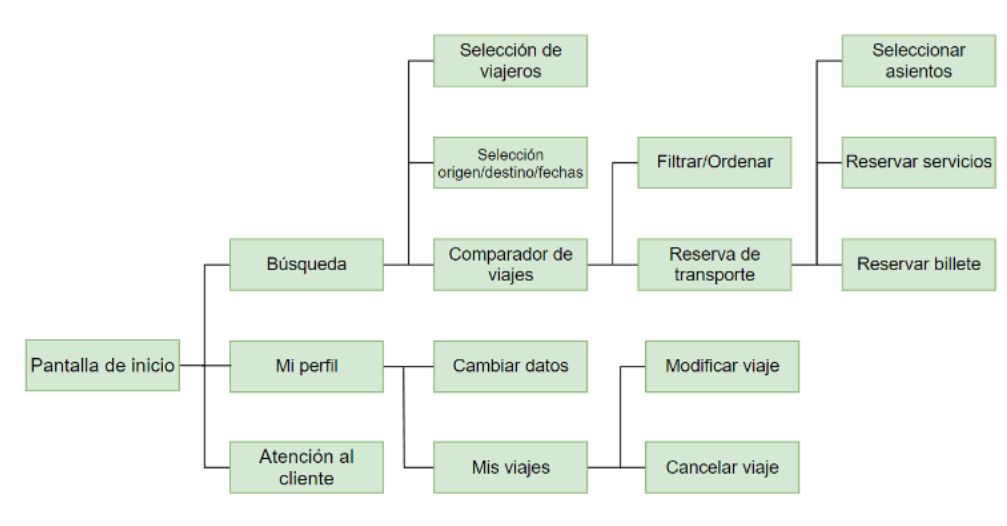
\includegraphics[width=0.8\linewidth]{./Imagenes/jerarquia.png}
    \caption{Diagrama de jerarquías de funciones}
    \label{fig:jerarquias}
\end{figure}

\subsection{Orden general en que se usarán los elementos}

\begin{enumerate}

    \item Cambiar la configuración de idioma y moneda.
    \item Acceder a \textit{Atención al cliente} desde la \textit{Página principal}.
    \item Acceder a \textit{Perfil} desde la \textit{Página principal}.
    \item Funcionalidad principal: comparar distintas opciones de transportes según las necesidades.

\end{enumerate}

\subsection{Principios y patrones usados}

\begin{itemize}

    \item \textbf{Principio de proximidad.} Al agrupar elementos similares conseguimos que el usuario sepa que están relacionados, facilitando así el aprendizaje. Así como mejorar la memorabilidad, ya que el usuario puede relacionarlos mentalmente y recordarlos como grupo.
    Por ejemplo, la moneda y el idioma se han puesto cerca porque son dos elementos de configuración.    
    \item \textbf{Principio de cierre.} Tendemos a buscar un único elemento simple.
    En nuestro caso, hemos puesto una barra deslizante para ver todo el contenido de la página.
    \item \textbf{Principio.} Los elementos de configuración, perfil y ayuda emplean los elementos de otros sistemas para que sea más fácil y rápido.
    \item \textbf{Principio de visibilidad y feedback.} La interfaz emplea distintos mecanismos para transmitir su estado actual y las acciones posibles en un determinado momento.
    Por ejemplo, en la pantalla de Comparador, pone los pasos que quedan para finalizar el proceso.
    \item \textbf{Ley de Von Restorff.} Destacar una funcionalidad por encima del resto.
    En la Página principal, queremos dar más importancia a la barra de búsqueda ya que es el objetivo principal de nuestra aplicación

\end{itemize}


\section{Escenarios key path}
Los escenarios key path presentan de forma desarrollada los distintos pasos que una persona tendría que seguir para realizar acciones comunes dentro del programa. En esta sección se presentan escenarios pensados desde el punto de vista de las personas creadas en el hito 2.

\subsection{Marta planea un viaje por Italia}

Marta quiere ir a las distintas ciudades del norte de Italia de la gira de Francesca, por lo que abre en el ordenador la aplicación, inicia sesión y en la parte de búsqueda selecciona dos viajeros, ya que va a ir con su hermano. También selecciona como origen Madrid, como destino la primera ciudad de la gira y las fechas que habían planificado quedarse en esa ciudad para luego ir a la próxima ciudad según la ruta diseñada. En este primer caso, ha tenido que filtrar los resultados en avión, ya que tienen que viajar de un país a otro para la primera ciudad y lo más rápido posible. Los resultados aparecen ordenados como predeterminados por fechas, así que no cambia la opción de ordenar. Finalmente reservan los billetes.
Para el resto de ciudades, hace el mismo procedimiento, a excepción de aquellas ciudades que por lo planificado tiene que contratar algunos medios de transportes o servicios específicos, como es el de camas para dormir apropiadamente. Para esto no ha puesto filtros de medios de transporte y antes de reservar el billete, reserva el servicio de camas (si tiene, sino busca otro transporte, pero lo mira en información antes) y ya reserva el billete.
Antes de reservar el billete, en cualquier caso, Marta ha tenido que mirar bien la zona de recogida, origen y destino del transporte disponible seleccionado para que se cumpla bien la planificación o modificarla y seleccionar los asientos contiguos de manera que ella y su hermano se sienten juntos.
Al final, cuando ya ha reservado todo ha entrado en la sección de su perfil de los viajes que ha realizado la compra de algún billete para comprobar que todo cuadra con su planificación y todo estaba correcto. Aunque luego ha tenido que volver a meterse en su perfil para cancelar un viaje ya que la cantante ha cancelado el concierto en esa ciudad y modificar la fecha del día que iba a ir al siguiente viaje para adelantarla, que ha sido fácil porque sólo ha tenido que cambiar la fecha del día de embarque que había aún dos billetes disponibles e incluso ha sido más barato.

\subsection{Marta cambia el viaje por motivos económicos}

Como dentro de poco son los exámenes y Marta está agobiada, su amiga Pili le ha sugerido ir a Ibiza el fin de semana posterior a los exámenes para relajarse. A Marta le ha parecido bien la idea así que coge su móvil y abre la aplicación con la sesión ya iniciada y en la sección de búsqueda selecciona dos viajes y como origen Madrid, destino Ibiza y de fecha el fin de semana acordado. Como anda justa de dinero a los resultados ha tenido que filtrarlos por precio menor de 50 euros y ordenarlos por precio creciente, pero no aparece ningún resultado. Como no podía subir más su presupuesto, se le ocurre quitar el destino para ver qué lugares le alcanza el dinero y ha visto que había un descuento para dos personas a Palma de Mallorca. Así que  después de que Pili cediera al cambio de planes, finalmente selecciona Palma de Mallorca, los asientos y reserva el viaje.

\subsection{Isabel busca un viaje accesible}

Mientras espera el desayuno, Isabel recibe una llamada de su jefe informando sobre la conferencia para la inclusión de niños con discapacidad y la necesidad de encontrar un sustituto para la potente original. Debido a la urgencia, Isabel acepta la propuesta y decide ponerse a buscar transporte para asistir a la conferencia. Para ello abre la aplicación en el móvil e inicia sesión en su cuenta. Debido a su condición física y a la premura de la situación, en la sección de filtros de la aplicación selecciona la opción “persona con discapacidad física” para buscar los transportes que se encuentren mejor adaptados. Además, en la sección tipo de transporte, selecciona “vuelos”.

Una vez aplicado el filtro de búsqueda, explora las diferentes opciones de vuelos y se cerciora mirando la información detallada que son vuelos con facilidades, sobre todo, para personas que requieren silla de ruedas.
Considerando que se trata de un viaje no planificado e inmediato, Isabel prioriza los vuelos más económicos que cumplan con los requisitos previos. Para ello se apoya en el apartado de  ordenador de viajes por “precio más bajo” para una mayor facilidad en su búsqueda.

Una vez realizada la compra del billete, Isabel se siente satisfecha con la utilidad y simplicidad de la aplicación y se dirige a casa a preparar su maleta.

\subsection{Isabel tiene problemas con la compra de su viaje}

Carmen e Isabel tienen el deseo de asistir a la exposición de un artista emergente que les gusta mucho. Ahora que el artista regresa a Madrid con una nueva exposición, deciden viajar un par de días para no perderse la oportunidad.

Isabel abre la aplicación, inicia sesión y comienza a buscar opciones de trenes de Renfe, que se adapten lo mejor posible a sus horarios y necesidades. Eligen Renfe debido a que Carmen tiene descuentos con esa compañía. A la hora de utilizar el buscador, establecen como destino, “Madrid”; número de viajantes, “2”; y filtro de medio de transporte, “trenes” de la empresa “Renfe”. 
Por otro lado, la exposición durará un mes entero, por lo que no tienen fechas concretas sobre las que realizar el viaje. Para ello utilizan la opción de la aplicación de filtrado por un intervalo de tiempo específico, en este caso un mes. De la misma forma, utilizan el ordenador de viajes por “precio más bajo” para buscar los trenes más baratos, teniendo una búsqueda más rápida e intuitiva.

Una vez seleccionados y comprados los billetes, Isabel espera durante un período de tiempo razonable a recibir los billetes a través de su correo electrónico vinculado a su cuenta. Ante la falta de recepción de los mismos, se pone en contacto con el servicio de atención al cliente facilitado por la aplicación. Tras explicar su situación, le informan que están teniendo problemas con la gestión de los billetes y le asegura que resolverán el problema de forma manual en pocos minutos. 
Como prometido, un momento después, Isabel y Carmen recibieron sus billetes, confirmando así su compra exitosa.

\section{Prototipado}

Tras analizar los distintos requisitos, grupos funcionales y escenarios key-path, cada miembro del grupo presenta distintos prototipos para ofrecer distintos puntos de vista. Dentro de estos prototipos presentamos distintas pantallas y cada uno ofrece su visión al respecto. Cada prototipo se dividirá en las distintas pantalla propuestas:

\subsection[Boceto de Alejandro]{Boceto de Alejandro\footnote{Carpeta con el boceto de Alejandro: \url{https://drive.google.com/drive/folders/1CLpkCqsbOiCKe3X4Alg8wcJb7H8soJQd?usp=drive_link}}}

\begin{itemize}
    \item\textbf{Página de inicio:} \\ En la página de inicio se encuentran solo el buscador (dividido en destino, fechas de ida y vuelta y número de pasajeros) y una serie de ofertas para incentivar a los usuarios a probar destinos nuevos. El \textit{header} se mantendrá igual a lo largo de toda la página, componiéndose del logo de la página (el cual te lleva a la página de inicio), un acceso directo a las ofertas, otro a una sección de destinos populares y un acceso a la página de asistencia, junto a un icono de usuario que te lleva al inicio de sesión o a tu perfil. 
    \item\textbf{Comparador:} \\ El comparador mantiene la misma barra de búsqueda para poder cambiar las opciones, así como un desplegable de filtrado para poder filtrar por precio, medio de transporte, etc. y otro desplegable para ordenar por precios, tiempo y otras opciones. El comparador en sí se presenta en forma de tarjetas con distinta información de cada viaje.
    \item\textbf{Página de compra:} \\ La página de compra tiene un selector de asientos visual, con el color verde para espacios no ocupados, en rojo para los ocupados y los azules para los espacios reservados para personas con discapacidades físicas. Para diferenciar viajeros tendremos un desplegable que cambia los datos de los usuarios que vayan a viajar, desde 1 hasta N. Cada usuario rellenará sus datos y más tarde se puede seleccionar el método de pago.
    \item\textbf{Perfil de usuario:} \\ La página de perfil de usuario presenta el mismo \textit{header} ligeramente modificado, con la ausencia del botón de perfil de usuario. Dentro del perfil podemos modificar los datos del usuario, así como ver las reservas actuales y modificarlas. al final de la página podremos ver la reseña de cada viaje y sus calificaciones, seguido de un título y una descripción.
\end{itemize}



\subsection[Boceto de Carlos]{Boceto de Carlos\footnote{Carpeta con el boceto de Carlos: \url{https://drive.google.com/drive/folders/1D3gLVOxOGFO8uPkvK2vkMU2Do2ZOVNPp?usp=drive_link}}}

\begin{itemize}
    \item\textbf{Página de inicio:} \\ En el diseño de la página principal Carlos propone poner el logo en el medio justo encima de la barra de búsqueda, la barra de búsqueda contiene apartados de origen, destino, fecha de salida y fecha de llegada, estas fechas pueden ser flexibles añadiendo un desplegable que aparece el calendario y un botón para poner +- días. También en la barra de búsqueda hay un apartado para poner el número de viajeros.
    El botón de buscar en la barra de búsqueda esta a la derecha del todo.
    En la parte superior derecha hay un botón para ir el perfil del usuario, un botón para ir a los viajes del usuario y dos iconos, uno para cambiar el idioma y otro para la moneda.
    Debajo de la barra de búsqueda Carlos propone tres apartados, uno con viajes de oferta, otro con propuestas y el último con destinos populares.
    
    
    \item\textbf{Comparador:} \\ Carlos propone en la página del comparador de viajes mantener la misma barra de búsqueda que en el la página de inicio en la parte superior.
    A la izquierda propone poner los filtros, permitiendo rangos 
    Debajo de la barra de búsqueda hay botones para elegir el medio de transporte y al lado un botón para ordenar los viajes mostrados.
    Carlos propone dos columnas de tarjetas de viaje en medio, la primera con los viajes de ida y la segunda con los viajes de vuelta.
    Cada tarjeta con la información del viaje, salida, llegada, origen, destino, paradas/escalas.
    Carlos propone que a la derecha de las columnas aparezca un mapa donde aparezca la ruta seguida y las paradas/escalas marcadas. Los puntos unidos por una flecha.
    
    \item\textbf{Página de compra:} \\ Carlos propone una pantalla intermedia de resumen de reserva. 
    En esta página aparecen a la izquierda tres tarjetas. La primera con la información completa del viaje de ida, debajo de esta tarjeta otra con la información del viaje de vuelta y por último debajo una tarjeta con el precio total del viaje.
    Debajo de las tarjetas Carlos propone un botón de añadir pasajeros al viaje.
    Al lado de cada tarjeta de viaje aparece el asiento seleccionado y a la derecha un dibujo del interior del transporte donde se puede seleccionar el asiento y aparecen los que ya están seleccionados. 
    A la derecha del todo Carlos propone que aparezca la lista con los servicios que se pueden seleccionar a mayores para el viaje.
    
    \item\textbf{Página de ``Mis reservas'':} Carlos propone que a la izquierda aparecen las tarjetas de los viajes pasados y el más reciente aparezca más grande con la información más relevante, con botones de ver estado del viaje, modificar viaje y cancelar viaje. 
    Carlos propone que a la derecha aparece un mapa en grande donde aparezca la ruta del viaje seleccionado a la izquierda.
    
    
    \item\textbf{Perfil de usuario:} \\ Carlos propone que los datos de los usuarios aparezcan a la izquierda en una lista con un cuadro de texto a la derecha donde aparezcan los datos introducidos.
    Debajo de los datos del usuario, Carlos propone tres botones. un botón de suscribirse a la versión prime de la aplicación, un botón de modificar los datos introducidos y un botón de cancelar la cuenta.
    A la derecha Carlos propone que aparezca un botón que te lleve a la pantalla de viajes del usuario.
    

    \item\textbf{Modificar viaje:} \\ Carlos propone que esta pantalla sea igual a  la pantalla de reserva y te permita seleccionar más o menos servicios y cambiar los asientos.
    \item\textbf{Cancelar viaje:} \\ Carlos propone un pop-up donde te pregunte porque motivo cancelar el viaje, con posibilidad de poner otro caso en forma de texto.
    Debajo aparecen botones de cancelar o no cancelar.
    
    
\end{itemize}
\subsection[Boceto de Daniel]{Boceto de Daniel\footnote{Carpeta con el boceto de Daniel: \url{https://drive.google.com/drive/folders/1s6A8aLfWLpiXH4j1sNpUaha3d3mf8XFg?usp=drive_link}}}


\begin{itemize}
    \item\textbf{Página de inicio:} \\ Diseño de la pantalla de inicio con aspectos parecidos a los demás. El diseño es simple, sin muchos elementos. Contiene los elementos necesarios para realizar un búsqueda como el destino, la salida, las fechas. También tiene otras opciones de búsqueda, número de pasajeros, si el viaje es solo ida y vuelos directos.
    \item\textbf{Comparador:} \\ Viajes disponibles se agrupan en ida y vuelta, para facilitar la búsqueda, filtros de búsqueda a la izquierda de las opciones disponibles y posibilidad de ordenar mediante diferentes factores las opciones disponibles (precio, duración de viaje, horario de salida).
    \item\textbf{Página de ``Mis reservas'':} \\ Una lista de los viajes reservados por el usuario. Por cada reserva, aparecen detalles, y también una opción para modificar datos de la reserva, y otro para cancelar la reserva
    
\end{itemize}

\subsection[Boceto de Guille]{Boceto de Guille\footnote{Carpeta con el boceto de Guille: \url{https://drive.google.com/drive/folders/1Gl75aNhKJPCpgOizfZxlmVY386eNbcU_?usp=drive_link}}}

\begin{itemize}
    \item\textbf{Página de inicio:} \\ El diseño se orienta a la interfaz típica de una página web, con su header, conteniendo el logo de la aplicación y las principales ventanas de acceso, el cuerpo de la página con la información que se quiere mostrar y un footer en el que se detalla la política de privacidad.
    
    La página de inicio diseñada por Guillermo se divide en tres secciones. La primera de ellas es la búsqueda de viajes, en la que se puede elegir el origen. el destino, las fechas en las que se va a realizar, indicar el número de asientos que se quieren ocupar y si se desea que el viaje sea accesible.
    Otra de las secciones que aparece es una breve descripción de la aplicación, indicando sus miembros y sus principales funciones.
    Por último, aparecen detallados los viajes que tienen los mejores precios.

    \item\textbf{Comparador:} \\ Guillermo optó por separar las vistas de los vuelos de ida y vuelta, haciendo que primero se seleccionan los de ida y en caso de que haya seleccionado ida y vuelta, los de vuelta. 
    
    Otra de las características del proceso de reserva es que se ha optado por una barra de progreso, en la que se detallan las distintas etapas del proceso de reserva. La primera de ellas es la elección del transporte, la segunda las características adicionales de la reserva y la tercera la selección del método de pago.

    La presentación de la información se realiza en forma de tarjetas, de modo que cada una de ellas va a referenciar a un viaje. La estructura de la tarjeta es muy sencilla. En primer lugar, aparece el icono del transporte a la izquierda (autobús, tren o avión), la hora de salida y de llegada, la compañía que lo opera y el precio (sin iva) del billete.

    Por otro lado, en la sección izquierda de la pantalla aparecen las distintas opciones por las que se pueden filtrar los viajes: tipo de transporte, intervalo horario, precio y viajes accesibles, así como la posibilidad de poder ordenarlos.
    \item\textbf{Página de compra:} \\ Tercera fase del proceso en la que se puede seleccionar el método del pago con el que se va a efectuar la compra. Puede hacerse tanto por tarjeta de crédito como por PayPal.
    En el caso de la tarjeta de crédito se solicita información tanto del titular de la tarjeta, como del número, el CVV y la fecha de caducidad.
    En el caso de PayPal se pide iniciar sesión con la cuenta de PayPal para poder realizar el pago.

    Tras introducir los datos necesarios, si el procesamiento del pago se ha realizado correctamente, aparece un mensaje en pantalla que indica al usuario que la reserva se ha realizado correctamente y que puede ser consultada en su perfil, en el apartado “Mis reservas”.

    \item\textbf{Página de ``Mis reservas'':} \\ Todas las ventanas del perfil van a tener una sidebar a la izquierda con un pequeño menú de navegación en el que se puede acceder a modificar los datos del perfil y a mis reservas.

    En el caso de la pestaña de mis reservas se ha optado por un diseño similar al de la comparación de viajes: mostrar la información en forma de tarjetas, detallando el medio de transporte en el que se va a realizar el viaje, la hora de salida de la ida y de la vuelta y los destinos entre los que se va a realizar el viaje.

    A la derecha de cada tarjeta se da la opción tanto de modificarla como de poder eliminarla.

    Si se hace click sobre la tarjeta de una reserva, aparece una nueva pantalla en la que se puede ver la información detallada de un viaje: los trayectos de ida y de vuelta, las fechas y la posibilidad de descargar los billetes.

    \item\textbf{Perfil de usuario:} \\ La pantalla del perfil se divide en dos secciones: una sidebar desde la que poder acceder a las funciones del perfil (mis reservas y modificar los datos) y una ventana principal en la que aparece la foto del usuario, junto a su nombre completo y apellidos. Debajo de esta información aparece información complementaria, como la dirección y el teléfono de la persona en caso de que haya que contactar.
    \item\textbf{Cancelar viaje:} \\ Dentro de la pestaña de Mis Reservas, al lado de cada una de las tarjetas aparece un botón que permite eliminar una reserva en caso de que el usuario lo desee.
\end{itemize}

\subsection[Boceto de Javier y Pablo]{Boceto de Javier y Pablo\footnote{Carpeta con el boceto de Javier y Pablo: \url{https://drive.google.com/drive/folders/1tK_ibzM1pp2TJYlYrToq9VKKUczw79f4?usp=drive_link}}}

\begin{itemize}
    \item\textbf{Página de inicio:} \\ Pablo y Javi trabajaron conjuntamente en un diseño del buscador con muchos elementos comunes al resto de compañeros. Decidieron un diseño limpio, poco cargado, con información justa y necesaria y con la diferencia de añadir una serie de casillas que designan un filtrado del viaje al inicio en función del tipo de persona que sea el cliente. Existen casillas de personas con más de 65 años y de carnet joven, la cual para viajes en tren, obtiene un descuento económico considerable, esto es importante para que el precio del viaje resulte descontado al iniciar la búsqueda. Además está la casilla de PMR(Persona con Movilidad Reducida) la cual consideramos más necesaria que nunca ya que normalmente no es hasta el final de una reserva de un viaje en bus o tren, en la que un cliente puede marcar que es una PMR. Esto dificulta mucho la reserva porque hay muchos trenes y buses que no están habilitados con asientos o espacios para estas personas o que ya están ocupados al haber escasez de ellos en algunos momentos. Por lo Pablo y Javi han decidido ponerlo al principio de la búsqueda para evitar que el cliente tenga que probar muchas opciones hasta encontrar una reserva potencial, algo que ahorra mucho tiempo y es muy sencillo de diseñar.
    
    \item\textbf{Comparador:} \\ Pablo y Javi establecieron la idea de que salieran los resultados de la búsqueda en tres secciones, una por cada tipo de transporte (avión, tren y autobús). De esta manera se ponen en pantalla todas las opciones disponibles y que a la hora de comparar se evita más el hecho de viajar de una página a otra comparando resultados. Un inconveniente es que se provoca una sobreestimulación al usuario al haber mucha concentración de información.
    Es importante para Pablo y Javier colocar el símbolo de la accesibilidad en la esquina superior derecha del resultado así como una flecha que indica el número de paradas, en la que si se hace click se abre una ventana con las paradas y sus horas. Así el usuario sabrá si en este caso, el medio de transporte está habilitado para PMR.
    
    \item\textbf{Página de compra:} \\ En este punto Pablo y Javi a la izquierda optaron por poner la información a rellenar de los pasajeros y a la derecha los datos del método de pago. Arriba al inicio, la información del viaje elegido con los asientos escogidos. Pablo y Javi creyeron conveniente que apareciera un pop-up al pulsar ``Pagar'' . En caso de que el proceso haya sido exitoso, solo aparece un mensaje de ``Éxito'' y varias opciones para descargar en primera instancia el recibo del pago y los billetes. Además de eso ambas cosas serán enviadas al correo electrónico para que no se pierda, luego se podrá acceder en el perfil del usuario, en sus reservas. En caso de fallo, no aparece nada, se marcarán los campos erróneos en rojo para que el usuario corrija la información propuesta.
    \item\textbf{Página de ``Mis reservas'':} \\ Se optó por un diseño sencillo de una sola página en la que salen las reservas de billetes. A la derecha de la reserva salen una serie de botones con opciones, de momento Pablo y Javi pusieron ``Anular'' y ``Detalles'', cuando se pulsa anular, se abre un pop-up donde el usuario enumera los motivos por lo que quiere cancelar la reserva, en este pop-up hay un botón en el cual habilita al usuario examinar los ficheros del ordenador, para que este pueda subir los ficheros solicitados a rellenar los las empresas de transportes(Iberia, Alsa, Renfe,...).

    \item\textbf{Cancelar viaje:} \\ Pablo y Javi optan por la misma opción descrita en la “Pantalla de reservas” pero también en la propia página de cancelar viajes.
\end{itemize}

\subsection[Boceto de Laura]{Boceto de Laura\footnote{Carpeta con el boceto de Laura: \url{https://drive.google.com/drive/folders/175YIjquOMOUuaC3SfTCDUe5mkSYAeiRE?usp=drive_link}}}

\begin{itemize}
    \item\textbf{Página de inicio:} \\ En el prototipo de la página principal, Laura optó por un diseño simple que cumpliese la consistencia externa con el resto de páginas de comparadores de viajes. Para ello ha propuesto una cabecera con el logo de la aplicación a la izquierda y a la derecha el ícono del usuario, que al hacerle clic accede a la página del usuario (se explica más adelante). 
    En el cuerpo de la página, Laura ha seguido con la consistencia externa, como se ha comentado anteriormente, teniendo los campos de lugar origen, lugar destino, la fecha de ida (con un formato específico), la fecha de vuelta y el número de viajeros. Al final, se encuentra el botón de buscar para dar paso a la ventana del comparador.
    En el pie de página plantea los botones de atención al cliente y de más información o preguntas frecuentes, con los logos que dan a entender la funcionalidad del botón.
    
    \item\textbf{Comparador:} \\ 

    En este prototipo del comparador, Laura, al igual que con el de la pantalla de inicio, lo ha diseñado siguiendo con la consistencia externa respecto a los comparadores de viaje.
    Laura ha decidido seguir manteniendo la cabecera igual que la del inicio, permitiendo que al hacer clic sobre el logo vuelva al inicio de la página y pueda hacer clic en el usuario para ir a la pantalla de usuario.
    En el cuerpo de la página, ha dividido la parte de la izquierda para los filtros que reducen los resultados para que aparezcan más específicos. Se muestran los filtros más relevantes y tiene la opción de que se puede visualizar más.
    En el centro de la pantalla, Laura ha decidido que al principio está la sección de ordenar que tiene cuatro botones, el de las dos flechas (significa que puede cambiar el orden de mayor a menor o al revés), del precio, de fechas (más próximas) y de duración (del trayecto). Al final de esta línea de botones, se sitúa el botón de volver atrás.
    Siguiendo con el centro de la pantalla, Laura ha decidido que los resultados de los viajes se muestre en un rectángulo que indique al principio en una etiqueta el tipo de transporte. Las posibles combinaciones de ida y vuelta con sus compañías, las horas, el lugar, la duración y el tipo de viaje (directo, con escalas o paradas, etc.). En la parte inferior a la derecha se sitúa el botón de ver el viaje con más detalle (pantalla de reserva, que se explicará más adelante), el precio (muy destacado para llamar la atención del usuario) y un botón de información (que al hacer clic sale una ventana emergente con los servicios disponibles, separados por ida y vuelta y la accesibilidad que ofrecen, si ofrecen).
    Al final de la página, se encuentran los botones de atención al cliente y más información, como en la pantalla de inicio.
    
    \item\textbf{Página de compra:} \\ En esta pantalla, Laura ha decidido dividirla en dos, la parte de la izquierda el resumen del viaje y la de la derecha el resumen de los gatos.
    En la parte izquierda, Laura ha propuesto poner el resumen del viaje con la compañía escogida, el tipo de transporte, la duración del viaje de ida y vuelta, y las ciudades. Debajo de estas están las secciones de información que se puede desplegar para ver la descripción del destino y origen con los lugares donde se coge el transporte y un poco de información. Debajo de la información están los servicios adicionales con sus precios, los que ha escogido el usuario están marcados en la checkbox con una cruz, pero en cualquier caso puede seleccionar los otros y los que ya no quieren quitarlos. Y finalmente, está la sección de descuentos y promociones que puede usar el usuario si es que hay.
    A la derecha, Laura ha decidido diseñar un resumen de todos los gastos y al final, el botón reservar los billetes.
    También propone los botones de volver atrás, de atención al cliente y de preguntas frecuentes como las anteriores pantallas.
    \item\textbf{Página de ``Mis reservas'':} En este caso, Laura ha optado por incluirlo en la misma pantalla que en la de usuario y es un resumen del viaje que pone origen y destino con el precio y las fechas. Tiene las opciones de modificar que sería la pantalla parecida a la de reservar y el comparador de viajes, la de cancelar (que te saldrá una ventana de si está seguro de que quiere cancelar el viaje) y la de visualizar el billete (muy parecida a la de reservar quitando el botón de reservar, el resto igual).
    \item\textbf{Perfil de usuario:} \\ En esta pantalla, Laura ha pensado un diseño que al principio te de la bienvenida con tu nombre de usuario y proceda con el resto de la página.
    A la izquierda de los campos de datos está la imagen que puede cambiar el usuario en cualquier momento.
    A la derecha ha pensado haya un menú desplegable con distintas opciones como datos personales, tus reservas y cuenta. 
    En la opción de datos personales Laura ha decidido que incluya los campos de nombre de usuario, nombre completo (separados nombres, primer apellido y segundo si tiene), edad y sexo.
    La opción de tus reservas ya ha sido explicada antes.
    La opción de cuenta ha propuesto mostrar el campo de correo (con la posibilidad de cambiarlo) y eliminar cuenta.
    Y, como las anteriores pantallas, propone los botones de volver atrás, de atención al cliente y de preguntas frecuentes.
    
\end{itemize}

\subsection[Boceto de Leire]{Boceto de Leire\footnote{Carpeta con el boceto de Leire: \url{https://drive.google.com/drive/folders/1UuyvH4UscltpxwordJf_IMLDTDp9Oekc?usp=drive_link}}}

\begin{itemize}
    \item\textbf{Página de inicio:} \\ En el prototipo de la página principal, Leire decidió centrarse en el diseño de una barra de búsqueda como objeto principal de la pantalla, en el que aparece el origen y destino deseados, las fechas, el número de pasajeros y si se quiere realizar el viaje sólo de ida o de ida y vuelta.
    En la parte de arriba de la pantalla encontramos el logo con el nombre de la empresa (si pinchas te llevaría a la página principal desde cualquier pantalla), a la izquierda, y un icono para el perfil, a la derecha.
    En el caso de pinchar sobre el icono del perfil, se desplegará una pestaña que permitirá al usuario ir a su información personal o cerrar sesión.
    Debajo de la barra de búsqueda encontraremos una serie de ofertas con los viajes más baratos actualmente. Así como las fechas de estos viajes y los precios, para una compra más rápida.
    Abajo a la derecha, tenemos el botón del chat. Si pinchas, se abre una ventana en la misma página para poder ponerse en contacto con atención al cliente (este botón lo tendremos en todas las ventanas).
    
    \item\textbf{Comparador:} \\ 
    En este caso, Leire dejó la barra de búsqueda de la pantalla principal por si se realizan cambios, para que sea más fácil para los usuarios modificar la información.
    Debajo de la barra de búsqueda, encontramos diferentes tarjetas con la información de los diferentes medios de transportes para el viaje elegido (fecha, hora, precio y si tiene escalas o es directo). Podemos filtrar la información mostrada con los diferentes filtros que tenemos en la parte izquierda de la pantalla (podemos filtrar por medio de transporte, ruta, precio, compañía, horas de salida y llegada…). También podemos elegir el orden en el que nos muestran las tarjetas (precio, duración…).
    
    \item\textbf{Página de ``Mis reservas'':} \\ En este caso, Leire ha optado por poner la foto del usuario a la izquierda con un botón debajo para cerrar la sesión.
    En la parte central de la pantalla, encontramos dos desplegables con las reservas activas y las pasadas.
    En el caso de pinchar sobre las activas, mostrará al usuario un resumen con la información de los viajes que tendrá próximamente. Así como darle la posibilidad de cancelar ese viaje.
    En el caso de pinchar sobre las pasadas, mostrará al usuario un resumen con la información de los viajes que ya ha realizado.
    
    \item\textbf{Perfil de usuario:} \\ En la pantalla del perfil, Leire ha decidido poner la foto del usuario en la parte izquierda, junto con un botón para acceder a los datos personales del usuario y otro para las reservas.
    En la parte derecha encontramos casillas para el nombre, apellidos, fecha de nacimiento, sexo y el resto de información del usuario. También da la posibilidad de cambiar estos datos.
    
\end{itemize}
\subsection[Boceto de Maria]{Boceto de Maria\footnote{Carpeta con el boceto de Maria: \url{https://drive.google.com/drive/folders/1mXz73K2l3AV1JRvOyf3aVBfp4IgAOCdD?usp=drive_link}}}

\begin{itemize}
    \item\textbf{Página de inicio:} \\ En la parte derecha del header cambiar idioma y moneda. También enlace a tu perfil de usuario y a tus reservas. 
    En la parte izquierda de header el logo de nuestra empresa y enlaces a las categorías de trenes, autobuses, vuelos.
    Sobre una imagen que cubre toda la pantalla excepto el header, un rectángulo con los campos para hacer la búsqueda. De izquierda a derecha: origen, destino, fecha de la ida, botón para añadir la vuelta si es sólo ida o en su defecto fecha de la vuelta, número de personas y botón de buscar. 
    
    \item\textbf{Comparador:} \\ En la parte derecha del header cambiar idioma y moneda. También enlace a tu perfil de usuario y a tus reservas. 
    En la parte izquierda del header el logo de nuestra empresa.
    Debajo de eso, aun en el header, mismos campos que la pantalla de inicio con la información de la búsqueda realizada.
    Pestañas para seleccionar transporte.
    En las opciones si destaca por algo (más rápida, más barata..).
    Encima de la lista de opciones.

    \item\textbf{Página de ``Mis reservas'':} \\ En la parte derecha del header enlace a tu perfil de usuario. En la parte izquierda del header el logo de nuestra empresa.
    Justo debajo, el título “Tus reservas” y un poco más abajo, dos opciones en forma de pestaña: próximas y archivadas.
    La imagen cubre toda la mitad superior de la pantalla, incluyendo desde las pestañas hasta encima del header.
    En la mitad inferior dos secciones: en la izquierda una lista con las reservas del tipo seleccionado, cada una en un recuadro y con todos sus datos, y en la derecha, un recuadro vertical a modo de formulario para recuperar reservas hechas y asociarlas con la cuenta de usuario. El título es “Recupera tu reserva” y tiene dos campos: nº de reserva y email.
    
    \item\textbf{Perfil de usuario:} \\ En la parte izquierda del header el logo de nuestra empresa. 
    Debajo se lee el título “Tu cuenta”
    Debajo, una lista con títulos de secciones: Información personal, Tus reservas, Métodos de pago, Notificaciones y Recomendados. Pinchando en cada una de ellas te lleva a la pantalla correspondiente. En este prototipo aparece la sección “Información personal”.
    Hay una imagen de fondo en la mitad superior de la pantalla, incluye desde la primera sección de la lista hasta justo encima del header.
    En la mitad inferior derecha, un recuadro con un título que lee “Detalles del pasajero” y campos para actualizar los datos: Tratamiento Sr/Sra, Nombre, Apellidos, Email, Fecha de nacimiento, País/Región y Nº de teléfono. Por último al terminar todos los campos, un botón de “Actualizar datos”.
    
    
\end{itemize}


\subsection[Boceto de Rodrigo]{Boceto de Rodrigo\footnote{Carpeta con el boceto de Rodrigo: \url{https://drive.google.com/drive/folders/1DUsmP6Jo2ZFUitYpQU91Pd6CipjM2G4M?usp=drive_link}}}

\begin{itemize}
    \item\textbf{Página de inicio:} \\ En la parte superior, panel de busca rápida de ofertas para los diferentes medios de transporte. 
    Casillas de marcado de utilización de bonos o descuentos. 
    
    \item\textbf{Comparador:} \\ Selección de tipos de transporte además de un sistema de ordenación en la parte superior.
    Barra lateral independiente con diferentes filtros de búsqueda acumulables.
    
    \item\textbf{Página de compra:} \\ Pantalla dividida en dos partes. En la parte izquierda zona de selección de detalles adicionales requeridos para la reserva del billete, como podría ser el seguro, servicios,etc. Además de información correspondiente a los titulares del billete.
    En la parte derecha, información sobre el método de pago, documentación relacionada con el billete tras la compra y zona de valoración del servicio de la aplicación.
    
    \item\textbf{Página de ``Mis reservas'':} \\ Tarjetas para los diferentes viajes con la información principal visible. Además de contar con la opción de ``más detalles'' para una mayor visión de las características del billete.
    Sistema de agrupación de billetes pasados y billetes que todavía no han sido usados los cuales se podrán modificar o anular.
    
    \item\textbf{Perfil de usuario:} \\ Pantalla dividida en dos partes. La parte izquierda, un panel de control con la foto del usuario y opciones de perfil como la configuración de notificaciones de la aplicación, ``suscripciones'' para ver las diferentes ofertas de suscripción disponibles, ``mis reservas'' para acceder directamente a la sección de tus reservas realizadas y ``cerrar sesión'' para salir de la cuenta.
    La parte derecha está conformada por los datos personales del usuario, además de las opciones de ``cancelar cuenta'' y ``guardar cambios'' en caso de que se quiera modificar los datos.
    
\end{itemize}

\subsection[Boceto de Sergio]{Boceto de Sergio\footnote{Carpeta con el boceto de Sergio: \url{https://drive.google.com/drive/folders/1Iw0kasuToaGSr-NjqgJBwVrCVe-GpAl1?usp=drive_link}}}

\begin{itemize}
    
    \item\textbf{Página de inicio:} \\ Con el objetivo de tener la máxima simplicidad en la pantalla de inicio, Sergio pensó que el centro de la pantalla debería ser ocupado por un simple botón que te llevase al comparador. Esto pone el foco sobre la principal utilidad de la aplicación. Además, siguiendo los principios de la jerarquía, habría un botón de perfil arriba a la derecha, con el que se podría acceder a los datos del usuario en caso de haber iniciado sesión o a la pantalla para iniciarla o registrarse en el caso de no tener cuenta o no haber accedido nunca. Por último, justo a la izquierda de este botón encontraríamos el botón de atención al cliente, el cuál abriría un desplegable con un chat y con otros datos de contacto, como el correo o el teléfono de la empresa.
    \item\textbf{Comparador:} \\ En este caso, Sergio optó por poner el filtrado por búsqueda en la mitad superior de la pantalla. Para mantener la consistencia externa con respecto al resto de comparadores, ha elegido el orden de origen-destino-fechas-acompañantes en este buscador. La opción de fechas abriría un calendario para poder seleccionar de manera más simple, pero igualmente se podría meter por teclado. En caso de dejar alguno de los apartados libres, buscaría las opciones que consideremos preferentes con respecto a los apartados rellenados. En la mitad inferior encontraríamos los resultados de la búsqueda anterior. En caso de no haber rellenado nada tendríamos las ofertas destacadas que creyéramos que pueden interesar al usuario. En la parte izquierda, tendríamos los diferentes filtros y ordenaciones que ofrece nuestra aplicación. Estaría flotando para poder bajar entre los diferentes viajes sin que varíen los filtros. Cada viaje estaría dentro de una Card, las cuales contienen los datos de mayor importancia para el usuario. A la izquierda habría una imagen a decidir entre el destino o la compañía. En la parte de info tendríamos datos básicos como el origen con la fecha y hora de salida, y el destino con los mismos datos de llegada. Además se podrá ver el tiempo de viaje y el aeropuerto tanto del origen como del destino. Junto a esta información podremos ver el precio. Esto será lo más destacado de la tarjeta, pues es uno de los atributos más importantes del viaje. A la derecha de esto tendremos los servicios que ofrece este tren, como por ejemplo si es accesible para personas con discapacidad o si cuenta con baños, si éstos son accesibles, etc. Como en la anterior pantalla, está en la parte superior el botón para acceder a los datos del perfil o de inicio de sesión y el botón para usar la atención al cliente. Además, se ha añadido un botón a la derecha para poder volver a la pantalla principal.
    \item\textbf{Página de compra:} \\ Esta sería una pantalla simple, ya que simplemente saldrían las cartas de los viajes de ida y de vuelta que se han elegido, para que pueda verificar que todos los datos son correctos. En caso de confirmar, el usuario accedería a una plataforma de pago externa a la aplicación. En la parte de arriba habría en la izquierda los botones para acceder al perfil del usuario y al lado para poder ver la atención al cliente. En la parte izquierda estaría el botón para ir a la pantalla anterior.
    \item\textbf{Perfil de usuario:} \\ Este es el prototipo que se vería en el caso de que el usuario haya iniciado sesión. Se vería a la izquierda la foto de perfil, y junto a ella los datos personales del usuario, a definir. Pero entre ellos podrían estar el nombre, los apellidos, el DNI y algunos datos de contacto, como podrían ser el correo y el teléfono. Debajo de la información habría 2 botones, uno con la opción de modificar alguno de los campos y otro para poder borrar el perfil. A la derecha de estos datos podemos ver las reservas que ha realizado el cliente. Serían unas cards más pequeñas que en el caso del comparador, en la que se incluiría una cantidad de datos menor, pero destacando igualmente el precio. Junto a cada tarjeta habrían 2 botones, uno con la función de borrarla, que nos llevaría a la función de cancelado de viaje, el cuál informaría de si el usuario podría recuperar el dinero (total o parcialmente) o no. El otro botón es para poder acceder a la pantalla de modificar viaje, a través de la cual el usuario tendrá la opción (en el caso de ser posible) de cambiar el viaje por otro, aportando la diferencia de precios. Igual que en los anteriores prototipos, arriba están las opciones de acceder al perfil, al servicio de atención al cliente y de volver a la pantalla anterior.

\end{itemize}

\subsection{Conclusiones finales y prototipo final}

El día 8 de noviembre, nos reunimos todos en el laboratorio para comentar los prototipos y que cada uno explicase
la idea detrás del suyo. Tras esto, debatimos entre todos qué ideas podían ser más útiles a la hora de realizar los prototipos
finales y qué podemos integrar de cada prototipo. Al final los resultados a los que llegamos han sido los siguientes.

En el inicio de sesión \ref{fig:prot_ses} tendremos la opción de iniciar por nombre de usuario y contraseña, iniciar sesión con Facebook o de iniciar sesión con Google. Algunos elementos comunes a toda la página serán un \textit{header} con el logo y las opciones de cambiar de moneda, de idioma o ir al perfil, un \textit{footer} con el nombre de la compañía, un enlace al aviso legar y un enlace a la política de privacidad y botones flotantes con un chat de asistencia y un \textit{F.A.Q}.

En caso de que sea un usuario que aún no se haya registrado, en la página de registro (figura \ref{fig:prot_reg}) tendrá que introducir su nombre, apellidos, fecha de nacimiento, email, nombre de usuario y contraseña.

En la pantalla de inicio (figura \ref{fig:prot_inicio}) nos enfocamos en la búsqueda, poniendo en la barra principal las opciones de origen y destino, fecha de ida y vuelta y el número de asientos (con opción de poner el tipo de viajero), en esta pantalla también mostraremos ofertas de viajes. 

Una vez el usuario haya realizado una búsqueda llegará a la página del comparador (figura \ref{fig:prot_comp}). En esta ventana mantendremos la barra de búsqueda de la ventana anterior, añadiendo debajo botones por cada tipo de transporte disponible (para solo mostrar del tipo seleccionado o de todos los tipos si no se selecciona ninguno) y un desplegable de ordenación. A la izquierda tendremos una pestaña de filtrado con distintas opciones. Debajo de la barra de búsqueda tendremos una serie de círculos numerados que harán de indicador para que el usuario sepa cuantos pasos le faltan para poder terminar con su reserva. Debajo de este indicador tendremos tarjetas para los distintos viajes, indicando el tipo de transporte, la compañía, el tiempo de duración, la hora de salida y de llegada con sus respectivos destinos y el precio, junto a un icono de información. En el caso de que tengamos ida y vuelta, se mostrarán dos columnas. Tras seleccionar las tarjetas correspondientes le daremos al botón de siguiente para continuar con el procedimiento.

El siguiente paso será rellenar los datos de la reserva (figura \ref{fig:prot_reser}), donde podremos poner los datos de los distintos pasajeros, seleccionar servicios adicionales y seleccionar los asientos. Tras rellenar toda la información pulsaremos el botón de siguiente y continuaremos al último paso.

El último paso es el pago (figura \ref{fig:prot_pago}). En esta ventana se nos mostrará un resumen de la reserva, un mapa con el trayecto de ida (y otro con el de vuelta si se ha seleccionado vuelta) y las opciones de pago por tarjeta y PayPal, así como un resumen del coste con impuestos. Tras hacer el pago correctamente saldrá una ventana emergente (figura \ref{fig:prot_pago_popup}) con el número de reserva para indicar que todo ha ido bien.

Para ver las reservas de un usuario iremos al perfil (figura \ref{fig:prot_perfil}). En el perfil podremos modificar datos, ver las reservas y ver los datos del usuario. Dándole al botón de mis reservas nos llevará a la página con el mismo nombre (figura \ref{fig:prot_reservas_usuario}), donde veremos las reservas pendientes de ocurrir y otras ya pasadas. Para las reservas pendientes podremos modificarlas (dando al botón del lápiz contiguo) o cancelarlas (dando al botón de cruz contiguo).

Si pulsamos al botón en cruz, nos saldrá un mensaje (figura \ref{fig:prot_reservas_usuario_popup}) para confirmar la anulación y pidiendo un motivo para la misma.

Si pulsamos una tarjeta de una reserva, podremos ver los datos detallados de la misma (figura \ref{fig:prot_reservas_mod}) donde podremos descargar los billetes


Finalmente, si deseamos modificar nuestros datos de usuario desde nuestro perfil se nos llevaría a la página de modificación (figura \ref{fig:prot_usuario_mod}), donde podremos cambiar la foto de perfil, nombre, apellidos, fecha de nacimiento, documento de identificación y teléfono.

Por último, en el caso de que el usuario que inicie la sesión sea un usuario con discapacidad, la pestaña del comparador mostraría únicamente viajes accesibles, con
posibilidad de consultar los servicios accesibles que ofrece cada uno de los transportes (figura \ref{fig:prot_comp_dis}). Asimismo, tras seleccionar su viaje, pueden 
en la página de datos adicionales de la reserva solicitar asistencia en las estaciones (tanto de origen como destino) (figura \ref{fig:prot_reserva_dis})

\begin{figure}[H]
    \centering
    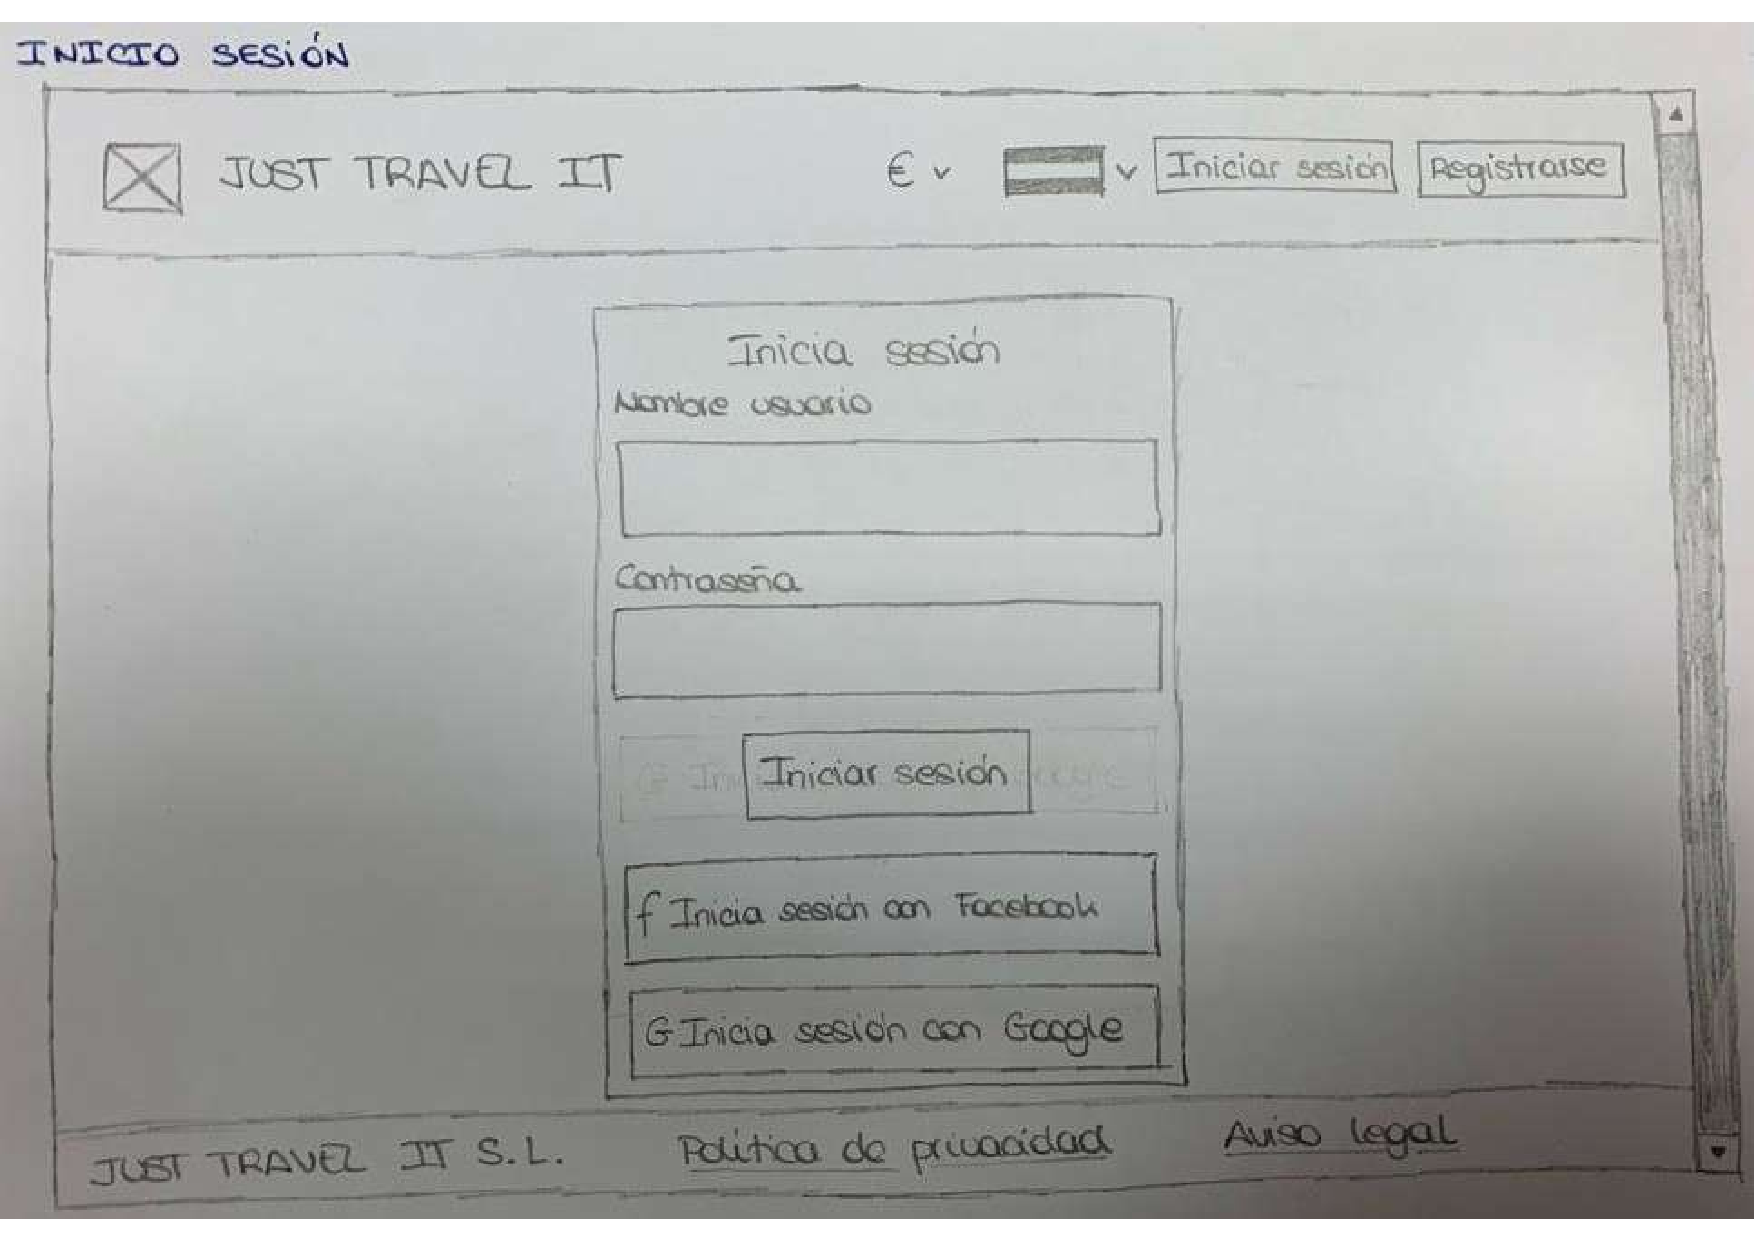
\includegraphics[page=1, width=0.9\textwidth]{./Imagenes/Prototipo/Prototipos definitivos - Iteracion I.pdf}
    \caption{Prototipo de página de inicio de sesión}
    \label{fig:prot_ses}
\end{figure}

\begin{figure}[H]
    \centering
    \includegraphics[page=2, width=0.9\textwidth]{./Imagenes/Prototipo/Prototipos definitivos - Iteracion I.pdf}
    \caption{Prototipo de registro de nuevo usuario}
    \label{fig:prot_reg}
\end{figure}

\begin{figure}[H]
    \centering
    \includegraphics[page=3, width=0.9\textwidth]{./Imagenes/Prototipo/Prototipos definitivos - Iteracion I.pdf}
    \caption{Prototipo de página de inicio}
    \label{fig:prot_inicio}
\end{figure}

\begin{figure}[H]
    \centering
    \includegraphics[page=4, width=0.9\textwidth]{./Imagenes/Prototipo/Prototipos definitivos - Iteracion I.pdf}
    \caption{Prototipo de página de comparador}
    \label{fig:prot_comp}
\end{figure}

\begin{figure}[H]
    \centering
    \includegraphics[page=6, width=0.9\textwidth]{./Imagenes/Prototipo/Prototipos definitivos - Iteracion I.pdf}
    \caption{Prototipo de página de Reserva}
    \label{fig:prot_reser}
\end{figure}

\begin{figure}[H]
    \centering
    \includegraphics[page=9, width=0.9\textwidth]{./Imagenes/Prototipo/Prototipos definitivos - Iteracion I.pdf}
    \caption{Prototipo de página de pago}
    \label{fig:prot_pago}
\end{figure}

\begin{figure}[H]
    \centering
    \includegraphics[page=8, width=0.9\textwidth]{./Imagenes/Prototipo/Prototipos definitivos - Iteracion I.pdf}
    \caption{Prototipo de página de pago con ventana emergente de haber pagado}
    \label{fig:prot_pago_popup}
\end{figure}

\begin{figure}[H]
    \centering
    \includegraphics[page=10, width=0.9\textwidth]{./Imagenes/Prototipo/Prototipos definitivos - Iteracion I.pdf}
    \caption{Prototipo de página de perfil de usuario}
    \label{fig:prot_perfil}
\end{figure}

\begin{figure}[H]
    \centering
    \includegraphics[page=12, width=0.9\textwidth]{./Imagenes/Prototipo/Prototipos definitivos - Iteracion I.pdf}
    \caption{Prototipo de página de reservas de un usuario}
    \label{fig:prot_reservas_usuario}
\end{figure}

\begin{figure}[H]
    \centering
    \includegraphics[page=11, width=0.9\textwidth]{./Imagenes/Prototipo/Prototipos definitivos - Iteracion I.pdf}
    \caption{Prototipo de página de reservas de un usuario con ventana emergente de anulación}
    \label{fig:prot_reservas_usuario_popup}
\end{figure}

\begin{figure}[H]
    \centering
    \includegraphics[page=13, width=0.9\textwidth]{./Imagenes/Prototipo/Prototipos definitivos - Iteracion I.pdf}
    \caption{Prototipo de página de consulta de una reserva}
    \label{fig:prot_reservas_mod}
\end{figure}

\begin{figure}[H]
    \centering
    \includegraphics[page=14, width=0.9\textwidth]{./Imagenes/Prototipo/Prototipos definitivos - Iteracion I.pdf}
    \caption{Prototipo de página de modificación de datos de un usuario}
    \label{fig:prot_usuario_mod}
\end{figure}

\begin{figure}[H]
    \centering
    \includegraphics[page=5, width=0.9\textwidth]{./Imagenes/Prototipo/Prototipos definitivos - Iteracion I.pdf}
    \caption{Prototipo de página de comparador de un usuario con discapacidad}
    \label{fig:prot_comp_dis}
\end{figure}

\begin{figure}[H]
    \centering
    \includegraphics[page=7, width=0.9\textwidth]{./Imagenes/Prototipo/Prototipos definitivos - Iteracion I.pdf}
    \caption{Prototipo de página de reserva de un usuario con discapacidad}
    \label{fig:prot_reserva_dis}
\end{figure}

\section{Escenarios de validación}
Tras diseñar algunos bocetos y realizar el diseño final, ponemos algunos escenarios posibles para ver como se podrían solucionar o si es posible que afecten a 
nuestra aplicación:

\begin{escenario} % 1
    \centering
?`Qué pasaría si el usuario quiere buscar un viaje que sea directo? 
\begin{solucion} \centering
    \textbf{No contemplado}. De momento, el usuario no puede filtrar los transportes en función del número de paradas que tengan, tenemos que añadir filtro para buscar viajes directos.
\end{solucion}
\end{escenario}

\begin{escenario} % 2
    \centering
?`Qué pasaría si el usuario se equivoca introduciendo sus datos personales de perfil? 

\begin{solucion} \centering
    \textbf{Existe}. Puede modificar sus datos desde la pestaña de usuario dándole al botón de modificar.
\end{solucion}
\end{escenario}

\begin{escenario} % 3
    \centering
?`Que pasaría si un usuario está en la página del comparador y entra en la pantalla de perfil y quiere volver?

\begin{solucion} \centering
    \textbf{No contemplado}. De momento no contemplamos que se pueda volver a la pantalla anterior, tenemos que añadir botón de volver. 
\end{solucion}
\end{escenario}

\begin{escenario} % 4
    \centering
?`Que pasaría si un usuario está en la página de reservas y quiere volver a su perfil? 

\begin{solucion} \centering
    \textbf{No contemplado}. De momento no contemplamos que se pueda volver a la pantalla anterior, tenemos que añadir botón de volver. 
\end{solucion}
\end{escenario}

\begin{escenario} % 5
    \centering
?`Que pasaría si un usuario está en la página de una reserva concreta y quiere volver a la pantalla de todas sus reservas?

\begin{solucion} \centering
    \textbf{No contemplado}. De momento no contemplamos que se pueda volver a la pantalla anterior, tenemos que añadir botón de volver. 
\end{solucion}
\end{escenario}

\begin{escenario} % 6
    \centering
?`Qué pasaría si el usuario quiere modificar sus datos porque ha visto un error en su billete? 

\begin{solucion} \centering
    \textbf{No contemplado}.  No está diseñada la ventana pero el usuario podría desde su perfil modificar los datos de reserva y guardar sus cambios.
\end{solucion}
\end{escenario}

\begin{escenario} % 7
    \centering
?`Qué pasaría si el usuario se da cuenta de que el precio final que aparece no se corresponde con el del billete por la aplicación de impuestos?

\begin{solucion} \centering
    \textbf{No contemplado}. El precio que figure en los billetes debería aparecer con el IVA aplicado.

\end{solucion}
\end{escenario}

\begin{escenario} % 8
    \centering
?`Qué pasaría si el usuario quiere consultar una duda concreta?

\begin{solucion}
    \centering
    \textbf{Parcialmente contemplado}. Existe un botón de preguntas frecuentes pero no está implementado.
\end{solucion}
\end{escenario}

\begin{escenario} % 9
    \centering
?`Qué pasaría si el usuario quiere consultar la fecha de sus viajes?

\begin{solucion}
    \centering
    \textbf{No contemplado}. No está diseñada para ver las fechas en la sección de las reservas realizadas por el usuario.
\end{solucion}
\end{escenario}

\begin{escenario} % 10
    \centering
?`Qué pasaría si el usuario quiere consultar las fechas en las que se produce el viaje cuando está buscando?

\begin{solucion}
    \centering
    \textbf{Parcialmente contemplado}. El usuario puede consultar una gran cantidad de datos en las tarjetas, pero las fechas del viaje no figuran.
\end{solucion}
\end{escenario}

\begin{escenario} % 11
    \centering
?`Qué pasaría si el usuario quiere cambiar las fechas de una reserva?

\begin{solucion}
    \centering
    \textbf{Contemplado}. no puede porque puede cambiar el precio, las horas, el transporte (por lo tanto, los asientos disponibles). Para ello habría que anular la reserva y coger otra.
\end{solucion}
\end{escenario}


\section{Segunda iteración}
Tras estudiar el prototipo final de la primera iteración, detectamos distintos problemas o mejoras que podíamos hacer. En esta segunda iteración pretendemos 
mejorar la interfaz y arreglar errores o cosas que faltaban en la primera. Algunos de estos errores y faltas se encuentran contemplados en los escenarios de validación
realizados en la iteración anterior. \\

Otra de las mejoras que se pretende llevar a cabo es la realización de los escenarios keypath utilizando las nuevas interfaces que ya han sido corregidas en esta iteración,
de modo que esta etapa va a realizarse en un orden contrario al de la iteración anterior: en primer lugar se van a realizar las correcciones sobre los prototipos y 
posteriormente los escenarios keypath. \\

Por último y para cerrar esta iteración, se han realizado los prototipos interactivos en forma de vídeo y además se van a plantear los escenarios de validación 
anteriores (y algunos nuevos que consideremos necesarios) para comprobar si hemos podido realizar correctamente las modificaciones necesarias.

\subsection{Prototipo}
Las ventanas de inicio de sesión (figura \ref{fig:prot2_ses}) , registro de usuario (figura \ref{fig:prot2_reg}), de inicio (figura \ref{fig:prot2_inicio}), datos adicionales de reserva (figuras \ref{fig:prot2_reser} y \ref{fig:prot2_reserva_dis}),y pago (figura \ref{fig:prot2_pago} y \ref{fig:prot2_pago_popup}) no han sido modificadas.
En el caso de las ventanas que muestran los precios de compra, como el comparador (figuras \ref{fig:prot2_comp} y \ref{fig:prot2_comp_dis}) y la página de inicio (figura \ref{fig:prot2_inicio}) muestran los precios con el IVA ya aplicado.
Las ventanas de comparador (figura \ref{fig:prot2_comp}), perfil (figura \ref{fig:prot2_perfil}), ``Mis reservas'' (figura \ref{fig:prot2_reservas_usuario} y \ref{fig:prot2_reservas_usuario_popup}), consultar reserva (figura \ref{fig:prot2_reservas_mod}) y modificar datos de usuario (figura \ref{fig:prot2_usuario_mod}) ahora tienen un botón para volver a la ventana anterior.
Las ventanas para la página de soporte (figura \ref{fig:prot2_soporte}), modificar reserva (figura \ref{fig:prot2_reserva_mod}) y preguntas frecuentes (figura \ref{fig:prot2_faq}) han sido añadidas para completar los requisitos. Por último, en el caso de las ventanas del comparador (figuras \ref{fig:prot2_comp} y \ref{fig:prot2_comp_dis}) aparece un nuevo filtro para seleccionar si se desean viajes directos o no.
\begin{figure}[H]
    \centering
    \includegraphics[page=1, width=0.9\textwidth]{./Imagenes/Prototipo/Prototipos definitivos - Iteración II.pdf}
    \caption{Prototipo de página de inicio de sesión}
    \label{fig:prot2_ses}
\end{figure}

\begin{figure}[H]
    \centering
    \includegraphics[page=2, width=0.9\textwidth]{./Imagenes/Prototipo/Prototipos definitivos - Iteración II.pdf}
    \caption{Prototipo de registro de nuevo usuario}
    \label{fig:prot2_reg}
\end{figure}

\begin{figure}[H]
    \centering
    \includegraphics[page=3, width=0.9\textwidth]{./Imagenes/Prototipo/Prototipos definitivos - Iteración II.pdf}
    \caption{Prototipo de página de inicio}
    \label{fig:prot2_inicio}
\end{figure}

\begin{figure}[H]
    \centering
    \includegraphics[page=4, width=0.9\textwidth]{./Imagenes/Prototipo/Prototipos definitivos - Iteración II.pdf}
    \caption{Prototipo de página de comparador}
    \label{fig:prot2_comp}
\end{figure}

\begin{figure}[H]
    \centering
    \includegraphics[page=6, width=0.9\textwidth]{./Imagenes/Prototipo/Prototipos definitivos - Iteración II.pdf}
    \caption{Prototipo de página de Reserva}
    \label{fig:prot2_reser}
\end{figure}

\begin{figure}[H]
    \centering
    \includegraphics[page=8, width=0.9\textwidth]{./Imagenes/Prototipo/Prototipos definitivos - Iteración II.pdf}
    \caption{Prototipo de página de pago}
    \label{fig:prot2_pago}
\end{figure}

\begin{figure}[H]
    \centering
    \includegraphics[page=9, width=0.9\textwidth]{./Imagenes/Prototipo/Prototipos definitivos - Iteración II.pdf}
    \caption{Prototipo de página de pago con ventana emergente de haber pagado}
    \label{fig:prot2_pago_popup}
\end{figure}

\begin{figure}[H]
    \centering
    \includegraphics[page=10, width=0.9\textwidth]{./Imagenes/Prototipo/Prototipos definitivos - Iteración II.pdf}
    \caption{Prototipo de página de perfil de usuario}
    \label{fig:prot2_perfil}
\end{figure}

\begin{figure}[H]
    \centering
    \includegraphics[page=11, width=0.9\textwidth]{./Imagenes/Prototipo/Prototipos definitivos - Iteración II.pdf}
    \caption{Prototipo de página de reservas de un usuario}
    \label{fig:prot2_reservas_usuario}
\end{figure}

\begin{figure}[H]
    \centering
    \includegraphics[page=12, width=0.9\textwidth]{./Imagenes/Prototipo/Prototipos definitivos - Iteración II.pdf}
    \caption{Prototipo de página de reservas de un usuario con ventana emergente de anulación}
    \label{fig:prot2_reservas_usuario_popup}
\end{figure}

\begin{figure}[H]
    \centering
    \includegraphics[page=11, width=0.9\textwidth]{./Imagenes/Prototipo/Prototipos definitivos - Iteración II.pdf}
    \caption{Prototipo de página de consulta de una reserva}
    \label{fig:prot2_reservas_mod}
\end{figure}

\begin{figure}[H]
    \centering
    \includegraphics[page=13, width=0.9\textwidth]{./Imagenes/Prototipo/Prototipos definitivos - Iteración II.pdf}
    \caption{Prototipo de página de modificación de datos de un usuario}
    \label{fig:prot2_usuario_mod}
\end{figure}

\begin{figure}[H]
    \centering
    \includegraphics[page=16, width=0.9\textwidth]{./Imagenes/Prototipo/Prototipos definitivos - Iteración II.pdf}
    \caption{Prototipo de página de soporte}
    \label{fig:prot2_soporte}
\end{figure}

\begin{figure}[H]
    \centering
    \includegraphics[page=15, width=0.9\textwidth]{./Imagenes/Prototipo/Prototipos definitivos - Iteración II.pdf}
    \caption{Prototipo de página de modificación de datos de una reserva}
    \label{fig:prot2_reserva_mod}
\end{figure}

\begin{figure}[H]
    \centering
    \includegraphics[page=17, width=0.9\textwidth]{./Imagenes/Prototipo/Prototipos definitivos - Iteración II.pdf}
    \caption{Prototipo de página de preguntas frecuentes}
    \label{fig:prot2_faq}
\end{figure}

\begin{figure}[H]
    \centering
    \includegraphics[page=7, width=0.9\textwidth]{./Imagenes/Prototipo/Prototipos definitivos - Iteración II.pdf}
    \caption{Prototipo de reserva para usuarios con discapacidad}
    \label{fig:prot2_reserva_dis}
\end{figure}

\begin{figure}[H]
    \centering
    \includegraphics[page=5, width=0.9\textwidth]{./Imagenes/Prototipo/Prototipos definitivos - Iteración II.pdf}
    \caption{Prototipo de comparador para personas con discapacidad}
    \label{fig:prot2_comp_dis}
\end{figure}

\subsection{Escenarios keypath}
Tras haber realizado las correcciones pertinentes sobre los prototipos diseñados, se han utilizado como punto de partida para poder profundizar y completar los
escenarios keypath, dotándolos de mayor significado. \\

Para poder completarlos, se ha acompañado el texto con las interfaces de la aplicación diseñadas en esta iteración, explicando con flechas y otros elementos los pasos
que se han seguido para solventar la situación planteada en el escenario de forma más visual y descriptiva que el texto sólo.

\subsubsection{Marta planea un viaje por Italia}
“Marta quiere ir a las distintas ciudades del norte de Italia de la gira de Francesca, por lo que abre en el ordenador la aplicación, inicia sesión y en la parte de búsqueda selecciona dos viajeros, ya que va a ir con su hermano. También selecciona como origen Madrid, como destino la primera ciudad de la gira y las fechas que habían planificado quedarse en esa ciudad para luego ir a la próxima ciudad según la ruta diseñada. 
En este primer caso, ha tenido que filtrar los resultados en avión, ya que tienen que viajar de un país a otro para la primera ciudad y lo más rápido posible. Los resultados aparecen ordenados como predeterminados por fechas, así que no cambia la opción de ordenar. 
En el siguiente paso, Marta rellena sus datos y los de su hermano y selecciona los asientos contiguos de manera que ella y su hermano se sienten juntos.
Finalmente en el paso último de la reserva de billetes, mirando antes la zona de recogida del lugar de origen y destino seleccionados mediante los mapas para que se cumpla bien la planificación y tener en cuenta para los siguientes billetes del resto de ciudades.” (figura \ref{fig:Marta1})
\begin{figure}[h]
    \centering
    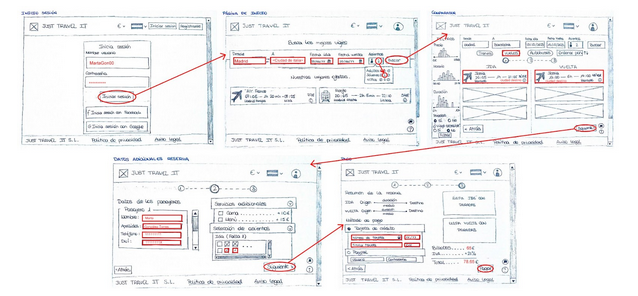
\includegraphics[width=0.7\textwidth]{Imagenes/Keypath/Marta1.png}
    \caption{Inicio de sesión y reserva}
    \label{fig:Marta1}
\end{figure}

“Para el resto de ciudades, hace el mismo procedimiento, a excepción de aquellas ciudades que por lo planificado tiene que contratar algunos medios de transportes 
o servicios específicos, como es el de camas para dormir apropiadamente. Para esto no ha puesto filtros de medios de transporte y antes de reservar el billete, 
reserva el servicio de camas (si tiene, sino busca otro transporte, pero lo mira en información antes) y ya reserva el billete.” (figura \ref{fig:Marta2})
\begin{figure}[h]
    \centering
    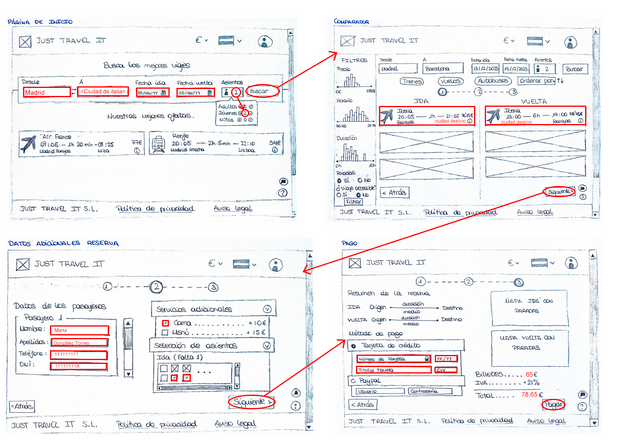
\includegraphics[width=0.6\textwidth]{Imagenes/Keypath/Marta2.png}
    \caption{Nueva reserva con servicios adicionales}
    \label{fig:Marta2}
\end{figure}

“Al final, cuando ya ha reservado todo ha entrado en la sección de su perfil de los viajes que ha realizado la compra de algún billete para comprobar que todo 
cuadra con su planificación y estaba correcto.” (figura \ref{fig:Marta3})
\begin{figure}[h]
    \centering
    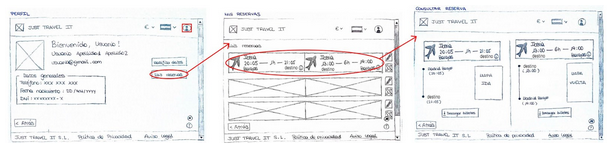
\includegraphics[width=0.7\textwidth]{Imagenes/Keypath/Marta3.png}
    \caption{Comprueba datos reserva}
    \label{fig:Marta3}
\end{figure}

“Marta ha tenido que volver a meterse en su perfil para cancelar un viaje ya que la cantante ha cancelado el concierto en esa ciudad.” (figura \ref{fig:Marta4}) “Debido 
a este último cambio, Marta modifica la fecha del día que iba a ir al siguiente viaje para adelantarla, que ha tenido que cancelar el viaje de la siguiente ciudad 
y reserva otro con las nuevas fechas. Con las prisas de que solo quedaban dos asientos libres, cree que ha puesto mal sus datos. Lo mira y efectivamente, 
están mal, así que modifica los datos de la reserva.” (figura \ref{fig:Marta5})
\begin{figure}[h]
    \centering
    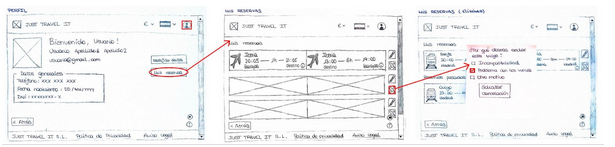
\includegraphics[width=0.7\textwidth]{Imagenes/Keypath/Marta4.png}
    \caption{Cancela una reserva}
    \label{fig:Marta4}
\end{figure}

\begin{figure}[h]
    \centering
    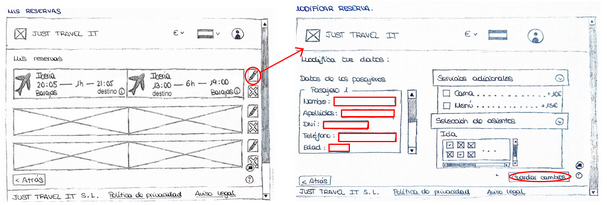
\includegraphics[width=0.7\textwidth]{Imagenes/Keypath/Marta5.png}
    \caption{Modifica datos reserva}
    \label{fig:Marta5}
\end{figure}

\subsubsection{Marta cambia el viaje por motivos económicos}
“Como dentro de poco son los exámenes y Marta está agobiada, su amiga Pili le ha sugerido ir a Ibiza el fin de semana posterior a los exámenes para relajarse. A 
Marta le ha parecido bien la idea así que coge su portátil y abre la aplicación con la sesión ya iniciada y en la sección de búsqueda selecciona dos viajes y 
como origen Madrid, destino Ibiza y de fecha el fin de semana acordado. Empieza ordenando los resultados con los precios crecientes pero ve que no son precios 
muy asequibles, así que aplica el filtro de precio a 50 euros máximo y no hay ningún resultado.” (figura \ref{fig:Marta6}) “Al final, cuando ya ha reservado todo ha entrado en la sección 
de su perfil de los viajes que ha realizado la compra de algún billete para comprobar que todo cuadra con su planificación y todo estaba correcto.”
\begin{figure}[h]
    \centering
    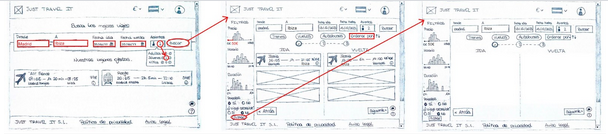
\includegraphics[width=0.6\textwidth]{Imagenes/Keypath/Marta6.png}
    \caption{Filtro sin resultados}
    \label{fig:Marta6}
\end{figure}

“Como no podía subir más su presupuesto, vuelve al inicio de la página mientras piensa y ve las ofertas que hay al principio y ve que ir a Palma de Mallorca sale 
20 euros la ida y vuelta cada uno. Así que después de que Pili cediera al cambio de planes, selecciona Palma de Mallorca, los asientos y reserva el viaje 
(hace el mismo proceso que el resto).” (figura \ref{fig:Marta7})
\begin{figure}[h]
    \centering
    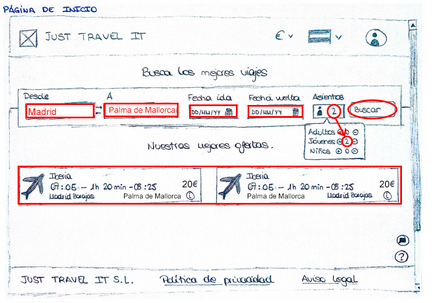
\includegraphics[width=0.35\textwidth]{Imagenes/Keypath/Marta7.png}
    \caption{Reserva de una oferta}
    \label{fig:Marta7}
\end{figure}

% \chapterA{Hito 5 - Prototipado digital}

\section{Introducción}
\section{Factor de forma, postura y métodos de entrada}

Debido a que en el anterior hito estaban correctamente no hemos modificado nada, pero lo
incluimos en la memoria para mantener todos los apartados necesarios a la hora de hacer un prototipado.

Hemos creado los elementos de datos (transportes, billetes y viajes), junto con
sus atributos (por ejemplo, horario en el caso de transportes) y las relaciones
con otros elementos de datos, como los transportes y los viajes.

Posteriormente, se ha realizado la traducción de los requisitos funcionales en
elementos funcionales. De forma que describimos las acciones que podemos
realizar añadiendo una acción, un objeto y un contexto.

\subsection{Factor de forma}
Nuestra aplicación estará diseñada para móvil y ordenador. Si se utiliza desde
el ordenador, la aplicación se utilizará en mayoritariamente en casa para poder
organizar el viaje tranquilamente, aunque también puede utilizarse en un
contexto de trabajo en el que el usuario esté en una oficina. Si se utiliza la aplicación desde el
móvil el contexto cambia mucho, ya que normalmente el usuario hará un uso de la aplicación rápido para poder consultar información en cualquier parte o momento.

\subsection{Postura}
Por un lado tenemos varias \underline{posturas soberanas} centradas en toda la
parte de buscar destino, comparación de precios, ofertas o destinos a los que
acudir según las preferencias indicadas por el usuario. Por otro lado
tendríamos una \underline{postura temporal} relacionada con el chat de soporte
o con diferentes dudas que le puedan surgir al usuario que necesiten ser
subsanadas, así como diferentes reseñas que los usuarios hayan escrito sobre
los diferentes destinos. Por último tendríamos una \underline{postura demonio}
relacionada con las diferentes notificaciones que puedan surgir mediante el uso
de la aplicación (como la calificación o respuesta a una reseña hecha) y las
preferencias indicadas por el usuario.

\subsection{Métodos de entrada}
En caso de que se utilice la aplicación vía ordenador, los métodos de entrada
serán el teclado y ratón, mientras que si se accede a la aplicación por el
móvil, el método de entrada será la propia pantalla del teléfono.

\section{Elementos de datos y funcionales}

Los elementos de datos serán la fuente de información de la aplicación
(transportes, billetes, etc). Los elementos funcionales son las acciones que
pueden ejercer los usuarios sobre dichos objetos. Tras analizar lo visto en
apartados anteriores, estos son los distintos elementos de datos y los
elementos funcionales.
\section{Elementos de datos}

En esta fase hemos definido los elementos de la interfaz que representarán los
requisitos identificados en la fase de identificación de requisitos.

Hemos creado los elementos de datos (transportes, billetes y viajes), junto con sus
atributos (por ejemplo, horario en el caso de transportes) y las relaciones con otros
elementos de datos, como los transportes y los viajes.

Posteriormente, se ha realizado la traducción de los requisitos funcionales en elementos
funcionales. De forma que describimos las acciones que podemos realizar añadiendo una acción,
un objeto y un contexto.

\subsection{Definición}

Tras un análisis de los errores cometidos en el hito anterior hemos definido los elementos
de la siguiente manera:

\begin{itemize}
    \item \textbf{Viaje}. Con este elemento representamos todos los datos sobre un desplazamiento
        concreto. Contará con los siguientes atributos:
        \begin{itemize}
            \item Fecha. Se marcará tanto el día de salida como el de llegada (pueden ser el mismo),
                con el formato en el orden correspondiente a la región (en España, \textit{dd/mm/aaaa}).
            \item Horario. La hora a la que sale el medio de transporte, además de la hora estimada de 
                llegada. El formato será \textit{HH:MM}, marcando la hora local del origen.
            \item Origen. Ciudad de la que sale el viaje, indicando la estación o aerpuerto correspondiente.
            \item Destino. Igual que con el origen, se guardará la ciudad de destino junto al lugar concreto.
            \item Accesibilidad. Si es un viaje accesible para personas con discapacidad o no.
            \item Transporte. El medio utilizado para viajar, en nuestro caso \textit{Avión}, \textit{Tren} o
                \textit{Autobús}.
        \end{itemize}

        Un viaje tendrá asociados tantos billetes como plazas tenga.

    \item \textbf{Billete}. Es el elemento que se paga para tener acceso al \textit{Viaje}. En caso de reservarse asientos
        para varias personas, se considerarán como el mismo \textit{Billete}, con los datos correspondientes de cada comprador.
        Poseerá los atributos siguientes:
        \begin{itemize}
            \item Precio. Cantidad de dinero en la moneda correspondiente que ha pagado el usuario por el \textit{Viaje}.
            \item Usuarios. Datos necesarios para identificar a los viajantes (definido posteriormente).
            \item Asientos. Plazas asignadas a cada uno de los usuarios.
            \item Servicios adicionales. Servicios contratados por uno o varios compradores para utilización durante el
                el \textit{Viaje}.
        \end{itemize}
        Cada \textit{Billete} está asociado a un transporte.

    \item \textbf{Usuario}. Persona que utiliza la aplicación, o que es partícipe de algún \textit{Viaje} (puede ser
        añadida a uno por otro \textit{Usuario}). Contará con los siguientes atributos:
        \begin{itemize}
            \item Nombre. Una cadena de caracteres con el nombre completo de la persona.
            \item Documento de identidad. Una cadena de caracteres correspondiente al documento identificativo de la
                la región pertinente al \textit{Usuario}.
            \item Fecha de nacimiento. Formato usado en la región desde la que se utiliza la aplicación (en España por ejemplo,
                sería \textit{dd/mm/aaaa}).
            \item Correo electrónico. Método para contactar con el \textit{Usuario} en caso de ser necesario (por ejemplo, al
                enviar los billetes, o en caso de que se tenga que notificar la cancelación de un viaje). Será una cadena de
                caracteres que será confirmada a través de un correo electrónico.
        \end{itemize}
        Un usuario tiene uno o varios viajes asociados.

\end{itemize}

\section{Elementos funcionales}
\section{Grupos funcionales y jerarquías}

En esta fase, una vez definidos los elementos de datos y funcionales, vamos a
organizarlos agrupándolos en unidades funcionales que nuestras personas el
trabajo en una tarea y la transición entre tareas. Para mostrarlo de manera más
visual hemos realizado un diagrama en árbol, para el que hemos usado el
programa \underline{\href{https://www.drawio.com/}{draw.io}}. Tras un análisis, 
hemos obtenido el resultado que observamos en la figura \ref{fig:jerarquias}, el cuál explicamos a 
continuación:

\subsection{Jerarquías}

\subsubsection*{Inicial}

La primera jerarquía, la cuál podemos observar en la figura \ref{fig:jerarquias1}, es la de buscar y
reservar viajes, la funcionalidad principal de nuestra aplicación. En el apartado \textit{Inicio}
debemos elegir el origen, destino, fecha de ida, fecha de vuelta, número de
acompañantes y pinchar en el botón de buscar. Una vez pinchado el botón de buscar, nos lleva al
\textit{Comparador}, que nos muestra las diferentes opciones de viaje para la ida y la vuelta y que podemos
ordenar por precio y duración. Una vez seleccionado cómo lo queremos ordenar los muestra los viajes
según el criterio elegido. También se pueden filtrar por duración, escalas y accesibilidad. Al
igual que en la ordenación nos mostraría las opciones resultantes tras el filtrado. Durante todo
este proceso tenemos la opción de visualizar la información del viaje de cada uno de
los trayectos mostrados. Una vez seleccionados los viajes deseados, debemos elegir los asientos,
rellenar los datos de los pasajeros, seleccionar los servicios adicionales y confirmar los datos.
Una vez se haya realizado el paso anterior, se procederá al pago. En el apartado \textit{Pago} se
deberán rellenar los datos de pago (tarjeta o \textit{PayPal}) y confirmarlo. Una vez completado el pago,
la reserva ya está confirmada.

\begin{figure}
      \centering
      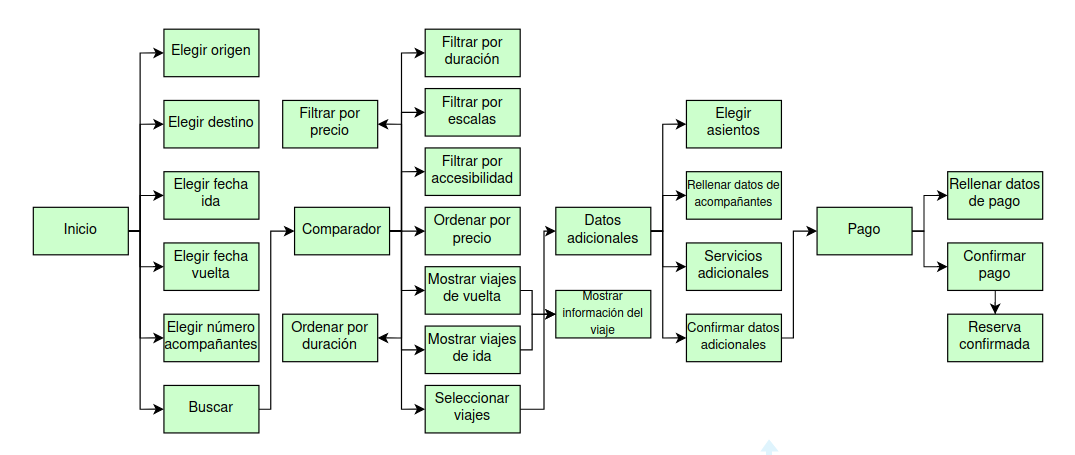
\includegraphics[width=0.8\linewidth]{./Imagenes/jerarquia-viaje.png}
      \caption{Diagrama de jerarquía para la reserva de un viaje}
      \label{fig:jerarquias1}
\end{figure}

\subsubsection*{Perfil}

En el apartado \textit{Perfil}, cuya jerarquía podemos ver en la figura \ref{fig:jerarquias2},
podemos acceder pulsando el botón de la esquina superior derecha en caso de haber iniciado sesión. Cuenta
con las siguientes opciones:

\begin{itemize}
      \item \textit{Modificar datos.} Nos muestra los datos actuales con la opción de cambiarlos. Después
            de modificarlos debemos confirmar los cambios.
      \item \textit{Mostrar los datos del usuario.} Nos muestra los datos personales del usuario como
            el nombre, los apellidos, el correo electrónico, el teléfono, la fecha de nacimiento
            y el DNI.
      \item \textit{Cerrar sesión.} Cierra la sesión del usuario actual.
      \item \textit{Mis reservas.} Muestra la información de las reservas pasadas y de las activas. Así
            como, la posibilidad de modificar y cancelar las reservas activas. Si se desea
            modificar la reserva, te da la posibilidad de elección de asientos, cambiar los datos
            de los pasajeros y seleccionar servicios adicionales. Después de modificar los datos
            deseados, debemos confirmar los cambios. Si se desea cancelar la reserva, se debe
            indicar cual/es de los billetes se quiere anular, el motivo y confirmar la cancelación.
\end{itemize}

\begin{figure}
      \centering
      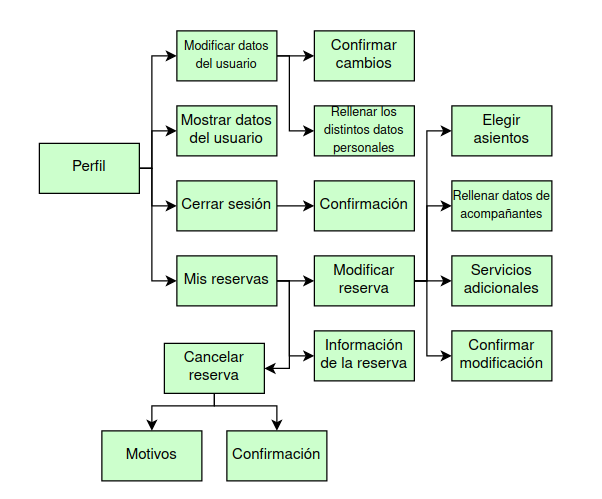
\includegraphics[width=0.8\linewidth]{./Imagenes/jerarquia-perfil.png}
      \caption{Diagrama de jerarquía para \textit{Perfil}}
      \label{fig:jerarquias2}
\end{figure}

\subsubsection*{Iniciar sesión}

En caso de querer iniciar sesión habría que pulsar el botón de la esquina superior derecha no teniendo
sesión iniciada. De esta manera accederíamos a la jerarquía de la figura \ref{fig:jerarquias3}, que
cuenta con las siguientes características.

\begin{itemize}
      \item Si el usuario tiene una cuenta, le pedirá el correo electrónico y contraseña antes
            de confirmar el inicio que le llevará a la página web con la sesión iniciada.
      \item Si el usuario no tiene cuenta, le dará la opción de crearla. Le llevará a la página
            de registro donde tendrá que rellenar los datos personales pedidos y confirmar el
            registro. Una vez creada la cuenta, iniciará sesión con sus credenciales.
\end{itemize}

\begin{figure}
      \centering
      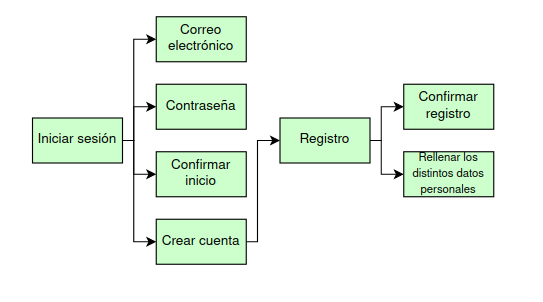
\includegraphics[width=0.8\linewidth]{./Imagenes/jerarquia-registro.png}
      \caption{Diagrama de jerarquía para el inicio de sesión y el registro}
      \label{fig:jerarquias3}
\end{figure}

\subsubsection*{Soporte/FAQ}

Desde cualquier punto de la aplicación se podrá acceder tanto a la pantalla \textit{Soporte} como
a la de \textit{Preguntas frecuentas}. La jerarquía de éstas se pueden ver en la figura \ref{fig:jerarquias4}.
Contamos con un apartado de \textit{Preguntas frecuentes} en el que podemos encontrar las preguntas
más frecuentes realizadas por los usuarios. En el caso de que la duda o cuestión del usuario no se
encuentre resuelta en el apartado anterior, también se cuenta con el apartado \textit{Soporte}. En
este apartado podemos encontrar tres opciones dependiendo de las necesidades del usuario:

\begin{itemize}
      \item \textit{Teléfono.} Nos muestra el número de contacto, así como, el horario de
            atención.
      \item \textit{Chat.} Nos permite enviar y recibir mensajes a atención al usuario.
      \item \textit{Mensajería.} Nos pide los datos de contacto como el nombre, el correo
            electrónico, el número de reserva y el mensaje que queremos envíar, para posteriormente
            enviarlo al equipo de atención al cliente.
\end{itemize}

\begin{figure}
      \centering
      \includegraphics[width=0.8\linewidth]{./Imagenes/jerarquia-soporte.png}
      \caption{Diagrama de jerarquía para \textit{Soporte} y \textit{Preguntas frecuentes}}
      \label{fig:jerarquias4}
\end{figure}

\subsection{Principios y patrones usados}

Algunos de los principios que hemos usado a la hora de diseñar son los siguientes:

\begin{itemize}

      \item \textbf{Principio de proximidad.} Este principio nos dice que cuando ciertos elementos están próximos, el cerebro interpreta
            que están relacionados. Esto facilita tanto el aprendizaje como la memoribiliadad de cara al usuario. Este principio lo usamos en prácticamente
            todas las ventanas, ya que la mayoría poseen varios botones u opciones relacionadas que son agrupables.
      \item \textbf{Consistencia interna.} Dentro de la aplicación mantenemos todos los elementos que posean la misma funcionalidad con apariencias iguales
            o similares. Esto lo hemos aplicado en el los fondos de la aplicación, en el uso de las \textit{Cards} para los viajes, en la fuente de letra, los
            botones, etc. De esta manera, se facilita que el usuario perciba las potencialidades de los elementos de la interfaz.
      \item \textbf{Consistencia externa.} Es importante mantener funcionalidades que se encuentra en otros sistemas para que los usuarios usen sus conocimientos
            de esos sistemas y no haya fricción cognitiva. Esto lo vemos por ejemplo en el \textit{Perfil}, que como en la mayoría de aplicaciones se encuentra en la parte
            superior a la derecha.
      \item \textbf{Ley de Hick.} Esta ley nos dice que el tiempo que hay que invertir para tomar una decisión incrementa con el número de opciones disponibles y la complejidad
            de éstas. Por eso, es importante dividir las tareas complejas en varios pasos. Esto lo aplicamos al realizar la reserva de un viaje, ya que ésta cuenta de varios
            pasos (\textit{Comparador}, donde se muestran todos los viajes disponibles; \textit{Reserva}, donde el usuario pone los datos adicionales del viaje, como los asientos
            o el resto de servicios; \textit{Pago}, donde el usuario rellena los datos referentes al pago para confirmar la reserva).
      \item \textbf{Principio de libertad y control del usuario.} En todos los aspectos intentamos dar el máximo control y libertad al usuario. Esto lo hacemos poniendo un botón para volver a la anterior
            pantalla en la mayoría de páginas y, por ejemplo, permitiendo la modificación o cancelación de las reservas hechas.
      \item \textbf{Principio de cierre.} Este principio nos dice que nuestro cerebro tiene tendencia a identificar patrones secuenciales, que constan de planteamiento, desarrollo y cierre,
            el cuál debe ser natural, una continuación del proceso que estábamos siguiendo. Este principio lo usamos por ejemplo en las pantallas en las que hay que hacer \textit{scroll} hacia abajo,
            dejando algún elemento entrecortado para mostrar al usuario que hay más elementos debajo.
      \item \textbf{Regla del \textit{peak-end}} Esta regla es un sesgo cognitivo que nos dice que los momentos intensos y los momentos finales de
            de una experiencia tienen gran importancia al recordar eventos pasados, por eso es importante cuidar estos momentos. Al finalizar un proceso laborioso como
            puede ser el de reserva de un viaje, mostramos una pantalla de que ha sido correctamente reservado, dando una sensación de tranquilidad al usuario
            al final del proceso.

\end{itemize}

Dentro de cada una de las ventanas explicaremos en más profundidad los principios usados para cada ventana en concreto.
\section{Prototipado}

Figma es una herramienta muy potente de diseño que permite la creación de prototipos
digitales altamente interactivos. Por ello, hemos empleado esta herramienta para poder
prototipar nuestras interfaces desarrolladas en el hito anterior, además de mejorarlas
aplicando aquellos cambios que se han considerado necesarios. Estos cambios serán explicados
en esta sección, además de detallar también los principios de diseño que aparecen en cada
una de las interfaces.

\subsection*{Inicio}

La pantalla principal de nuestra aplicación (figura \ref{fig:it1_inicio}), como ya detallamos anteriormente, va a ser la de búsqueda,
en la que, a diferencia de lo planteado en el hito anterior, cualquier usuario va a poder realizar la
comparación de viajes (aunque no pueda finalizar sin tener que iniciar sesión o crearse una cuenta). Otro
de los cambios que además se ha realizado es ofrecer la posibilidad a los usuarios que no se hayan registrado
como discapacitados de poder buscar viajes accesibles sin tener que aplicar el filtro en la siguiente página
(el comparador). Sin embargo, a pesar de estos cambios, la esencia de la ventana es la misma, se mantiene la
barra de búsqueda con todas las opciones que se pedían anteriormente (el origen, el destino, la fecha de ida,
la fecha de vuelta y el número de asientos) y para completar se muestran las mejores ofertas en forma de
tarjetas para que el usuario vea de forma mucho más visual toda la información que ahí se expone. En cuanto a
los patrones y principios que se han seguido para esta pantalla, son los siguientes:

\begin{itemize}
    \item \textbf{Principio de proximidad.} Todos los campos requeridos para realizar una búsqueda se encuentran
        cercanos entre sí, además de encuadrados bajo un marco, lo que indica al usuario que todo el contenido
        solicitado es necesario para comenzar una búsqueda de transportes. Relacionado a ello, aplica la Ley de
        Fitts (la distancia que tiene que ser recorrida para moverse de un campo a otro es muy pequeña).
    \item \textbf{Consistencia interna.} Las distintas tarjetas que se presentan para mostrar las ofertas de la
        aplicación en la página de inicio guardan y muestran la misma cantidad de información: el logo de la compañía
        que lo opera, la fecha del viaje, el precio, las horas de salida y llegada y las estaciones. También presenta
        consistencia en cuanto a la forma de la tarjeta y los colores que se utilizan.
    \item \textbf{Consistencia externa.} Al igual que en la gran mayoría de las aplicaciones, cuando el usuario tiene la sesión
        iniciada en la página, puede acceder a su perfil pulsando sobre el botón de usuario situado en la esquina
        superior derecha.
    \item \textbf{Principio de visibilidad.} Del mismo modo que en el caso anterior, puede consultarse el estado en el que
        se encuentra la aplicación si en la esquina superior derecha te sale la opción de iniciar sesión o de
        registrarse (sesión no iniciada) o el icono del perfil (sesión iniciada).
\end{itemize}

\begin{figure}[H]
    \centering
    \includegraphics[page=1, width = 0.8\textwidth]{Imagenes/hito_5/it1.pdf}
    \caption{Página \textit{Inicio}}
    \label{fig:it1_inicio}
\end{figure}

\subsection*{Comparador}

La pantalla del comparador (figura \ref{fig:it1_comparador}) no ha sufrido cambios con respecto al hito anterior, pero se ha cambiado el planteamiento
con respecto al hito anterior. Como ya hemos visto, dentro de la opción de búsqueda puedes seleccionar viajes
accesibles (aunque no seas una persona con discapacidad), apareciendo todos los viajes ya filtrados sin necesidad
de aplicar el filtro. Además, otra de las mejoras que se han realizado respecto a los prototipos en papel es hacer
que el botón de información de cada una de las tarjetas de los viajes muestre un \textit{pop-up} con la información más en
detalle del viaje: la información de las paradas que realiza (en caso de que las haya), la información del viaje
(la misma que se muestra en la tarjeta original), información de la compañía que opera el viaje (breve descripción
y un enlace a la página web), así como también los servicios adicionales que se ofrecen en el viaje. Se ha añadido
la funcionalidad de la ordenación de los viajes. En cuanto al contenido anterior de esta pantalla no se han realizado
modificaciones puesto que se ha considerado que la información que ya se mostraba tanto en los viajes como en los
filtros a aplicar era la necesaria. Una vez comentado el contenido de esta pantalla y las modificaciones que han
sido efectuadas, vamos a centrarnos en la identificación de los distintos patrones y principios que se han seguido
en el diseño de esta interfaz:

\begin{itemize}
    \item \textbf{Principio de proximidad.} Todas las tarjetas de los viajes de ida se encuentran bastante próximas entre
        sí y separadas de las tarjetas de viajes de vuelta, que entre sí también se encuentran cercanas, lo que
        indica que pertenecen a dos grupos distintos y claramente diferenciados. Por otro lado y aislado a este caso,
        el principio de proximidad también se aplica en el caso de las opciones de filtrado, ya que se encuentran
        todas agrupadas y próximas en la columna izquierda de la pantalla.
    \item \textbf{Consistencia interna.} al igual que ocurría con las ofertas que aparecían en la página de inicio, todas
        las tarjetas de viajes tanto de ida como de vuelta tienen la misma consistencia, puesto que la información
        que muestran y la tipografía y los colores que se utilizan son los mismos en todas las tarjetas. Otro de los
        ejemplos de la consistencia podemos observarlo en los filtros. Como puede apreciarse, aquellos filtros que se
        refieren a rangos (como el rango horario, el rango de precios o la duración), tienen el mismo formato de
        presentación, una barra en la que puedes moverte para seleccionar el filtro y unas barras que indican la
        cantidad de viajes que existen con esos valores.
    \item \textbf{Consistencia externa.} Además de la ya mencionada ubicación del botón del perfil (en la parte
        superior derecha de la pantalla), otras de las opciones que aparecen en esta pantalla y que guardan
        consistencia con la gran mayoría de las aplicaciones son los botones de Atrás y Continuar, ya que aparecen
        respectivamente en la parte izquierda y en la derecha de la aplicación, indicando la sensación de avance
        (derecha) y retroceso (izquierda).
    \item \textbf{Principio de visibilidad.} Uno de los mecanismos que tiene esta pantalla para informarte del estado de la
        misma es destacar el borde de aquellos viajes (tanto de ida como de vuelta) que hayas seleccionado, pudiendo
        conocer rápidamente las opciones que has escogido.
    \item \textbf{Ley de Hick.} Con la finalidad de no realizar un proceso de compra demasiado complejo y lleno de información,
        hemos decidido dividir el proceso en tres etapas: una primera etapa de selección de los viajes deseados,
        una segunda de datos y servicios adicionales y una tercera en la que se muestra un resumen y se procede al
        pago del viaje.
    \item \textbf{Efecto Zeigarnik.} Aunque la idea de dividir el proceso en distintas etapas se trate de un resultado de la
        Ley de Hick para intentar que sea mucho menos tedioso, la idea de mostrar la etapa del proceso en la que te
        encuentras para saber los pasos necesarios para finalizar es resultado de la aplicación directa del Efecto
        Zeigarnik.
    \item \textbf{Principio de libertad y control del usuario.} El usuario en todo momento tiene el control de la aplicación
        y puede decidir cuándo avanzar y cuándo retroceder en todo momento si ha detectado que ha cometido un error
        o bien quiere explorar otras opciones.
\end{itemize}

\begin{figure}[H]
    \centering
    \includegraphics[page=10, width = 0.8\textwidth]{Imagenes/hito_5/it1.pdf}
    \caption{Página \textit{Comparador}}
    \label{fig:it1_comparador}
\end{figure}

\subsection*{Datos adicionales}

Al finalizar el proceso de selección de los viajes que se quieren reservar, la siguiente pantalla (figura \ref{fig:it1_datos_adicionales}) que aparece es
la de datos adicionales, que incluye: los datos de los pasajeros, si se desean contratar servicios
adicionales (gratuitos o bien pagando un suplemento) y la selección de los asientos. En cuanto a las modificaciones
que se han realizado con respecto al hito anterior han sido principalmente una modificación de la opción de seleccionar
asiento, ya que la información representada no era muy clara y además no mostraba información más allá de los asientos
(sólo mostraba la información de los huecos libres, sin dar información de la ubicación - filas y columnas - ni si
tenía o no ventanilla). Es por ello que se ha planificado una mejora en la que ahora se muestra una leyenda de
colores en función del estado del asiento (hemos añadido además asientos que debido a su posición dentro del vehículo
suponen un incremento del precio, por lo que se van a destacar en otro color). En cuanto a los principios de diseño que
aparecen en esta pantalla, podemos destacar los siguientes:

\begin{itemize}
    \item \textbf{Principio de cierre}. Dentro de la opción de seleccionar los datos de los pasajeros, puede verse
        cómo el campo del teléfono se encuentra entrecortado, dando la sensación a los usuarios de que puede seguir
        bajando para poder rellenar más datos.
    \item \textbf{Consistencia interna.} Las dos pestañas que se tienen para poder seleccionar los asientos y los servicios
        adicionales tienen la misma forma y tipografía, dando a entender al usuario la información contenida en
        ellas está altamente relacionada y es necesaria para poder continuar con la reserva del viaje.
    \item \textbf{Consistencia externa.} Además de la ya mencionada ubicación del botón del perfil (en la parte superior
        derecha de la pantalla), otras de las opciones que aparecen en esta pantalla y que guardan consistencia
        con la gran mayoría de las aplicaciones son los botones de Atrás y Continuar, ya que aparecen respectivamente
        en la parte izquierda y en la derecha de la aplicación, indicando la sensación de avance (derecha) y retroceso
        (izquierda).
    \item \textbf{Ley de Hick.} Con el fin de no sobrecargar la pantalla de información, los datos adicionales que se necesitan
        para la reserva se han dividido en tres secciones, de las cuales dos de ellas son desplegables, haciendo que
        la cantidad de información que se solicita al usuario puede ser regulada por él en todo momento.
    \item \textbf{Efecto Zeigarnik.} La idea de mostrar la etapa del proceso en la que te encuentras para saber los pasos
        necesarios para finalizar es resultado de la aplicación directa del Efecto Zeigarnik.
    \item \textbf{Principio de libertad y control del usuario.} El usuario en todo momento tiene el control de la aplicación
        y puede decidir cuándo avanzar y cuándo retroceder en todo momento si ha detectado que ha cometido un error
        o bien quiere explorar otras opciones.
\end{itemize}

\begin{figure}[H]
    \centering
    \includegraphics[page=11, width = 0.8\textwidth]{Imagenes/hito_5/it1.pdf}
    \caption{Página \textit{Datos adicionales}}
    \label{fig:it1_datos_adicionales}
\end{figure}

\subsection*{Pago}

La última de las pantallas (figura \ref{fig:it1_pago}) necesarias para implementar la funcionalidad de realizar una reserva es la página de
pago. Una de las modificaciones realizadas (que ya mencionamos un poco anteriormente) es que antes de llegar a
esta página, si no tienes la sesión todavía iniciada, te requiere de hacerlo para poder continuar (al hacerlo te
vuelve a dirigir aquí con los datos de la compra que has realizado). En cuanto a las modificaciones realizadas
sobre la propia página, hemos mantenido la idea original de mantener los mapas de ida y de vuelta (mostrando el
itinerario a seguir) y pestañas en las que se dan dos posibles opciones de pago (tarjeta o PayPal). También
aparece el precio total del viaje, con el precio de los billetes más los suplementos que se hayan seleccionado
(servicios adicionales o asientos más caros). Sin embargo, a esto se le ha añadido un resumen de los viajes que
finalmente han sido seleccionados. Este resumen contiene las tarjetas de los viajes tanto de ida como de vuelta
y para cada una de ellas muestra la fecha, el origen, el destino y las fechas de salida y llegada. Además, cuando
se selecciona la opción de ver la información del vuelo, abre un \textit{pop-up} en el que se puede ver la información del
vuelo más detallada (los pasajeros que van a viajar, los asientos, los servicios que tiene disponibles y el precio). 

Otra de las modificaciones que se ha realizado es la información que aparece luego de confirmar la compra. En este
caso, hemos pasado de un \textit{pop-up} sencillo a una ventana en la que se muestra en detalle todo el resumen de la compra
que se ha realizado (las paradas, los destinos, las fechas, los pasajeros que van a viajar, los pasajeros y los
servicios adicionales que se han incluido en la compra). El mensaje con el número de la reserva diciendo que se ha
realizado correctamente se mantiene en la parte superior. Bajo esta información se encuentra un botón que da la
opción de continuar explorando nuevas opciones (lleva a la página de inicio). 

En cuanto a los principios de diseño que se han identificado (en ambas páginas, tanto en la referente a los datos
del pago como a la de confirmación de la compra), podemos encontrar los siguientes:

\begin{itemize}
    \item \textbf{Ley de Fitts.} Una vez decidido el método de pago con el que se va a realizar la reserva, los campos
        necesarios para efectuar la compra para cada uno de los métodos de pago se encuentran próximos entre sí
        (además de dentro de la misma pestaña), para poder facilitar al usuario moverse entre los distintos campos.
    \item \textbf{Consistencia interna.} La tipografía y los colores usados en las distintas opciones de pago (tanto en las
        pestañas como en los campos) es la misma, al igual que ocurre en el resumen de la compra (las tarjetas que
        representan los viajes de ida y de vuelta tienen la misma estructura y contienen la misma información para
        dársela al usuario). Esto también es aplicable al resumen de la compra, ya que la cantidad de información
        que se brinda en el viaje de ida es la misma que en el caso del viaje de vuelta.
    \item \textbf{Consistencia externa.} Como ya hemos visto en las etapas anteriores del proceso de reserva, se
        guarda cierta consistencia con el resto de aplicaciones, en las que se sobreentiende que el botón de retroceso
        de la página se encuentra en la parte derecha, mientras que en el caso de el de continuar (en este caso el
        botón de pagar) se encuentra en la parte derecha de la pantalla, dando la sensación de progreso.
    \item \textbf{Ley de Hick.} El número de opciones de pago que se ofrecen se encuentran separadas por pestañas,
        de modo que el usuario no se sobrecarga con una gran cantidad de información y de opciones con las que se
        puede realizar el pago.
    \item \textbf{Efecto Zeigarnik.} La idea de mostrar la etapa del proceso en la que te encuentras para saber los
        pasos necesarios para finalizar es resultado de la aplicación directa del Efecto Zeigarnik.
    \item \textbf{Principio de libertad y control del usuario.} El usuario en todo momento tiene el control de la aplicación
        y puede decidir cuándo avanzar y cuándo retroceder en todo momento si ha detectado que ha cometido un error
        o bien quiere explorar otras opciones.
    \item \textbf{Regla \textit{peak-end}.} Cuando se finaliza el proceso de reserva de la aplicación (\textit{peak}), se muestra a modo
        de finalización del proceso y para confirmar que todo se ha realizado correctamente una nueva ventana con
        un resumen de la información que se ha reservado.
\end{itemize}

\begin{figure}[H]
    \centering
    \includegraphics[page=8, width = 0.8\textwidth]{Imagenes/hito_5/it1.pdf}
    \caption{Página \textit{Pago}}
    \label{fig:it1_pago}
\end{figure}

\subsection*{Inicio de sesión}

Para poder realizar reservas nuevas en la aplicación, es necesario que se inicie sesión (figura \ref{fig:it1_inicio_sesion}) con
una cuenta válida y que se encuentre ya registrada en la aplicación. Para poder realizar una
reserva completa sí que es necesario realizar el inicio de sesión, aunque para buscar viajes
no es necesario, como ya hemos visto anteriormente. Con respecto al prototipo del hito anterior
no se han realizado modificaciones aparentes sobre esta página, ya que se ha considerado que
la información que se solicita al usuario es la necesaria. En cuanto a los principios de diseño
que se han seguido para la creación de esta ventana son los siguientes:

\begin{itemize}
    \item \textbf{Ley de Fitts.} Los campos que han de rellenarse para poder iniciar sesión en la
        aplicación (correo y contraseña) se encuentran próximos entre sí, facilitando al
        usuario en todo momento el desplazamiento de uno a otro, pudiendo aportar de forma
        sencilla la información que le es solicitada.
    \item \textbf{Consistencia interna.} La tipografía y la disposición empleada para destacar los campos
        del formulario es la misma tanto en el caso del correo como en el de la contraseña (en
        la parte superior del campo se encuentra un texto que describe lo que ha de escribirse
        en el formulario y luego puede apreciarse el campo propiamente dicho).
    \item \textbf{Consistencia externa.} La página de inicio de sesión guarda consistencia externa con
        el resto de páginas de este tipo de las otras aplicaciones, ya que los campos de inicio
        de sesión se encuentran en la parte superior de la ventana, al igual que inmediatamente
        debajo de ello se encuentra el botón de iniciar sesión (si ya has rellenado los campos).
        Justo debajo de iniciar sesión, en caso de que todavía no tengas una cuenta se da la
        opción de registrarse como un nuevo usuario de la aplicación. Este ejemplo de estructura
        puede verse en el inicio de sesión de \textit{Gmail}, entre otros.
    \item \textbf{Principio de visibilidad.} Como ya vimos anteriormente, uno de los estados que va a
        manejar nuestra aplicación es el hecho de si tienes la sesión iniciada actualmente o no.
        Para poder consultar esta información, se puede observar la esquina superior derecha. Si
        el icono que aparece es el perfil, la sesión se encuentra iniciada, mientras que en el
        caso contrario, se requerirá de que se inicie sesión.
\end{itemize}

\begin{figure}[H]
    \centering
    \includegraphics[page=5, width = 0.8\textwidth]{Imagenes/hito_5/it1.pdf}
    \caption{Página \textit{Inicio de sesión}}
    \label{fig:it1_inicio_sesion}
\end{figure}

\subsection*{Registro}

En el supuesto caso de que el usuario que quiera entrar a nuestra aplicación desee entrar para
poder realizar una reserva y no tenga una cuenta creada todavía, es posible darle la opción de
crearse una cuenta. Dentro de este nuevo formulario (figura \ref{fig:it1_registro}), al usuario le serán solicitados una serie
de datos adicionales (no solamente el correo y la contraseña). Estos datos adicionales han
variado con respecto al hito anterior, ya que se ha añadido nueva información para poder ofrecer
más facilidades al usuario, como por ejemplo, que a la hora de reservar un viaje, si tiene la
sesión iniciada, en los datos de los pasajeros se rellenará automáticamente la información del
primero de ellos con los datos que ya se tienen del usuario que se ha registrado en la aplicación.
En cuanto a los patrones de diseño que se han utilizado, hemos podido identificar los siguientes:


\begin{itemize}
    \item \textbf{Principio de proximidad.} Todos los campos que se necesitan para poder crear una nueva
        cuenta en la aplicación se encuentran próximos entre sí, permitiendo al usuario realizar
        movimientos muy cortos para desplazarse entre los distintos campos del registro.
    \item \textbf{Consistencia interna.} El fondo empleado tanto para cada uno de los campos así
        como la tipografía empleada para esta pantalla es consistente, ya que se mantiene dando
        una sensación de unidad en todo el conjunto de los datos.
    \item \textbf{Principio de visibilidad.} Como ya vimos anteriormente, uno de los estados que va a
        manejar nuestra aplicación es el hecho de si tienes la sesión iniciada actualmente o no.
        Para poder consultar esta información, se puede observar la esquina superior derecha. Si
        el icono que aparece es el perfil, la sesión se encuentra iniciada, mientras que en el
        caso contrario, se requerirá de que se inicie sesión.
\end{itemize}

\begin{figure}[H]
    \centering
    \includegraphics[page=2, width = 0.8\textwidth]{Imagenes/hito_5/it1.pdf}
    \caption{Página \textit{Registro}}
    \label{fig:it1_registro}
\end{figure}

\subsection*{Perfil}

El usuario puede entrar a su perfil y visualizar todos los datos que haya introducido en el
registro (figura \ref{fig:it1_perfil}). Un usuario no registrado en \textit{Just Travel It} no puede acceder a esta pantalla ya que
para ello es necesario como mínimo tener un perfil en la aplicación. El usuario tampoco podrá
acceder a la pantalla de perfil si no está con sus sesión iniciada, puede ocurrir que el usuario
esté registrado pero no tenga la sesión iniciada, para ello debe iniciar sesión. En cuanto a los
principios de diseño que aparecen en esta pantalla, se pueden resaltar los siguientes:

\begin{itemize}
    \item \textbf{Consistencia interna.} El color utilizado en los botones es el mismo al igual
        que la fuente y el tamaño de la letra. No solo entre los botones dentro de la pantalla
        sino con los del resto de la aplicación.
    \item \textbf{Ley de Fitts.} La información de cada tipo se mantiene agrupada en su grupo. Los
        datos personales están todos juntos en un párrafo, mientras que la información general
        en otro, de esta forma se le facilita al usuario el encontrar la información que desee
        más ágilmente.
    \item \textbf{Ley de Hick.} Se aprovecha la clasificación del tipo de información del cliente para no
        agrupar todo en un bloque. De esta manera, evitamos que el usuario no se sobrecargue de
        información.
    \item \textbf{Principio de libertad y control del usuario.} El usuario tiene el control de su
        información en todo momento, siempre que tenga la sesión iniciada. Con esta pantalla
        tenemos el objetivo de mostrarle al usuario toda la información que ha metido en la
        aplicación y con el botón de modificar su perfil le damos la posibilidad de cambiar su
        información cuando desee.
\end{itemize}

\begin{figure}[H]
    \centering
    \includegraphics[page=12, width = 0.8\textwidth]{Imagenes/hito_5/it1.pdf}
    \caption{Página \textit{Perfil}}
    \label{fig:it1_perfil}
\end{figure}

\subsection*{Modificar perfil}

Al usuario se le brinda la posibilidad de cambiar los datos de su perfil creado en \textit{Just Travel It} (figura \ref{fig:it1_mod_datos}). Podrá
modificar todos los campos rellenados en la creación del perfil. Ocurrirá lo mismo que en el \textit{Registro},
al modificar los datos, cuando se realice una reserva con la sesión iniciada se rellenaran los campos del perfil
en los campos adecuados a la reserva. Los principios empleados para la creación de esta ventana son:

\begin{itemize}
    \item \textbf{Consistencia interna.} La pantalla guarda consistencia sobre todo con la pantalla de la página de registro,
        los colores, tamaños, fuentes y tipografías se encargan de mantener la consistencia interna de estas pantallas.
    \item \textbf{Consistencia externa.} Se trata de la misma consistencia que podemos encontrar en \textit{Registro}.
    \item \textbf{Principio de proximidad.} Al ser igual que en \textit{Registro}, todas las preguntas se encuentran
        bastante próximas entre sí.
    \item \textbf{Principio de libertad y control del usuario.} El usuario en todo momento puede modificar todos
        sus datos introducidos en la aplicación.
    \item \textbf{Ley de Fitts.} Los campos que han de rellenarse para modificar el perfil se encuentran próximos
        entre sí y caben en la pantalla, por lo que no hay que hacer \textit{scroll} con el ratón, de este forma
        el usuario puede viajar con facilidad de un campo a otro.
\end{itemize}

\begin{figure}[H]
    \centering
    \includegraphics[page=4, width = 0.8\textwidth]{Imagenes/hito_5/it1.pdf}
    \caption{Página \textit{Modificar perfil}}
    \label{fig:it1_mod_datos}
\end{figure}

\subsection*{Mis reservas}

Se le ofrece al usuario con una sesión iniciada que pueda consultar la información de sus reservas (figura \ref{fig:it1_reservas})
activas así como de poder comprobar las reservas pasadas. En este punto es posible consultar, modificar o cancelar
una reserva. Pasamos a nombrar los principios utilizados en esta pantalla: 

\begin{itemize}
    \item \textbf{Consistencia externa.} Al igual que en la gran mayoría de las aplicaciones, cuando el usuario
        tiene la sesión iniciada en la página, puede acceder a su perfil pulsando sobre el botón de usuario situado
        en la esquina superior derecha.
    \item \textbf{Principio de libertad y control del usuario.} El usuario en todo momento tiene el control de la
        aplicación y puede decidir cuándo avanzar y cuándo retroceder en todo momento si ha detectado que ha
        cometido un error en cuanto a la página a donde quería acceder.
    \item \textbf{Principio de visibilidad.} Como ya vimos anteriormente, uno de los estados que va a manejar
        nuestra aplicación es el hecho de si tienes la sesión iniciada actualmente o no. Para poder consultar
        esta información, se puede observar la esquina superior derecha. Si el icono que aparece es el perfil,
        la sesión se encuentra iniciada, mientras que en el caso contrario, se requerirá de que se inicie sesión. Además,
        se reconoce rápidamente la asociación ida-vuelta de los viajes.
    \item \textbf{Principio de proximidad.} Todas las tarjetas de los viajes de ida se encuentran bastante próximas entre sí
        y separadas de las tarjetas de viajes de vuelta, que entre sí también se encuentran cercanas, lo que indica
        que pertenecen a dos grupos distintos y claramente diferenciados.
\end{itemize}

\begin{figure}[H]
    \centering
    \includegraphics[page=3, width = 0.8\textwidth]{Imagenes/hito_5/it1.pdf}
    \caption{Página \textit{Mis reservas}}
    \label{fig:it1_reservas}
\end{figure}

\subsection*{Consultar reserva}

Al usuario se le da la posibilidad de consultar su reserva (figura \ref{fig:it1_consulta_reserva}). Desde esta pantalla puede ver el viaje de ida y el
de vuelta, donde aparecen las tarjetas de los respectivos viajes, con las fechas, los días, la duración, la compañía,
la cantidad de pasajeros y la información adicional de la reserva. También se puede ver el mapa donde aparece la
ruta seguida en el viaje. Debajo del mapa se pueden consultar los datos de los pasajeros. Pasamos a nombrar los
principios utilizados en esta pantalla:

\begin{itemize}
    \item \textbf{Consistencia externa.} Al igual que en la gran mayoría de las aplicaciones, cuando el usuario
        tiene la sesión iniciada en la página, puede acceder a su perfil pulsando sobre el botón de usuario situado
        en la esquina superior derecha.
    \item \textbf{Consistencia interna.} La pantalla guarda consistencia sobre todo con la pantalla de la página
        resumen pago, los colores, tamaños, fuentes y tipografías se encargan de mantener la consistencia interna
        de estas pantallas.
    \item \textbf{Principio de proximidad.} Todos los campos que se necesitan para poder consultar una reserva en
        la aplicación se encuentran próximos entre sí, permitiendo al usuario realizar movimientos muy cortos para
        desplazarse entre los distintos campos.
    \item \textbf{Principio de libertad y control del usuario.} El usuario en todo momento tiene el control de la
        aplicación y puede decidir cuándo avanzar y cuándo retroceder en todo momento si ha detectado que ha cometido
        un error en cuanto a la página a dónde quería acceder.
    \item \textbf{Principio de visibilidad.} En esta pantalla se reconoce rápidamente la asociación ida-vuelta de los
        viajes.
    \item \textbf{Ley de Hick.} Con el fin de no sobrecargar la pantalla, los datos adicionales que se necesitan para
        la reserva se han dividido en dos secciones, haciendo que la cantidad de información que se muestra al
        usuario pueda ser regulada por él en todo momento.
\end{itemize}

\begin{figure}[H]
    \centering
    \includegraphics[page=6, width = 0.8\textwidth]{Imagenes/hito_5/it1.pdf}
    \caption{Página \textit{Consultar reserva}}
    \label{fig:it1_consulta_reserva}
\end{figure}


\subsection*{Modificar reserva}

Al usuario se le otorga la posibilidad de modificar las reservas que haya realizado en \textit{Just Travel It} (figura \ref{fig:it1_mod_reserva}). Podrá
modificar los datos del pasajero: nombre, apellidos, DNI y teléfono. Tendrá a su disposición dos menús desplegables,
uno para poder contratar servicios adicionales que no haya contratado con anterioridad y otro en el que podrá
modificar su asiento. Además cuenta con un boton de selección en la parte inferior izquierda para poder solicitar
asistencia en la estación correspondiente por si se olvido de marcarlo a la hora de realizar la reserva. Pasamos
a nombrar los principios utilizados en esta pantalla:

\begin{itemize}
    \item \textbf{Consistencia interna.} La pantalla guarda consistencia sobre todo con la pantalla de la página
        mis reservas, los colores, tamaños, fuentes y tipografías se encargan de mantener la consistencia interna de
        estas pantallas.
    \item \textbf{Consistencia externa.} Al igual que en la gran mayoría de las aplicaciones, cuando el usuario tiene
        la sesión iniciada en la página, puede acceder a su perfil pulsando sobre el botón de usuario situado en la
        esquina superior derecha.
    \item \textbf{Ley de Fitts.} Los campos que han de rellenarse para modificar el perfil se encuentran próximos
        entre sí y caben en la pantalla, por lo que no hay que hacer \textit{scroll} con el ratón, de este forma
        el usuario puede viajar con facilidad de un campo a otro.
    \item \textbf{Principio de libertad y control del usuario.} El usuario en todo momento tiene el control de la
        aplicación y puede decidir cuándo avanzar y cuándo retroceder en todo momento si ha detectado que ha cometido
        un error en cuanto a modificar los datos.
    \item \textbf{Principio de proximidad.} Todos los campos que se necesitan para poder modificar una reserva en
        la aplicación se encuentran próximos entre sí, permitiendo al usuario realizar movimientos muy cortos para
        desplazarse entre los distintos campos a modificar.
    \item \textbf{Principio de visibilidad.} Como ya vimos anteriormente, uno de los estados que va a manejar nuestra
        aplicación es el hecho de si tienes la sesión iniciada actualmente o no. Para poder consultar esta
        información, se puede observar la esquina superior derecha. Si el icono que aparece es el perfil, la sesión
        se encuentra iniciada, mientras que en el caso contrario, se requerirá de que se inicie sesión.
\end{itemize}

\begin{figure}[H]
    \centering
    \includegraphics[page=7, width = 0.8\textwidth]{Imagenes/hito_5/it1.pdf}
    \caption{Página \textit{Modificar reserva}}
    \label{fig:it1_mod_reserva}
\end{figure}

\subsection*{Soporte}

Si un usuario tiene alguna pregunta que no pueda ser abordada mediante el apartado de preguntas frecuentes previamente
mencionado (figura \ref{fig:it1_soporte}), ya sea debido a la naturaleza altamente específica de su problema o porque requiere una solución no
automatizada, o si experimenta algún inconveniente con la aplicación, tiene la opción de hacer clic en el incluíacono de
chat. Este icono se encuentra ubicado en la parte inferior derecha de cualquier pantalla de la página web, justo sobre
el icono de preguntas frecuentes.

Esta pantalla ha experimentado ciertas modificaciones con respecto al prototipo en papel. En este caso, hemos
expandido las funcionalidades de la sección de soporte, que anteriormente sólo incluía un asistente automatizado
de respuestas. La nueva sección ahora incorpora un canal de contacto telefónico, donde los usuarios pueden obtener
toda la información necesaria para comunicarse con un asistente personal. Además, hemos añadido una función de
mensajería que permite a los usuarios enviar mensajes y solicitudes directamente al equipo de asistencia al cliente,
que responderá con la mayor brevedad posible.

En cuanto a los principios de diseño que se han seguido para la creación de estas ventanas, son los siguientes:

\begin{itemize}
    \item \textbf{Principio de proximidad.} Todos los campos que se necesitan rellenar para poder enviar un nuevo
        mensaje, se encuentran próximos entre sí, permitiendo al usuario realizar movimientos muy cortos para
        desplazarse entre los distintos cuadros de texto. Relacionado a este principio, aplica la Ley de Fitts,
        donde la distancia que tiene que ser recorrida para moverse de un campo a otro es muy pequeña.
    \item \textbf{Consistencia interna.} Las distintas tarjetas que representan las formas de contactar con atención
        al cliente, tienen la misma estructura: un icono significativo, el significado de la tarjeta e información
        añadida en caso de ser necesaria. También presenta consistencia en cuanto a la forma de la tarjeta y los
        colores que se utilizan.
    \item \textbf{Consistencia externa.} Se guarda cierta consistencia con el resto de aplicaciones. Icono de
        perfil, botón de atrás y enviar, en el chat; el botón de enviar y el cuadro de texto para escribir (simulando
        el mismo que encontraríamos en un teléfono), una “X” que indica “cerrar el \textit{pop-up}”.
    \item \textbf{Feedback visual.} Una vez enviada la solicitud o mensaje al equipo de asistencia al cliente, el
        usuario recibirá un mensaje de confirmación con el objetivo de aclarar las dudas de si el mensaje ha sido
        enviado con éxito.
    \item \textbf{Principio de libertad y control del usuario.} El usuario mantiene el control total de la aplicación,
        teniendo la capacidad de avanzar o retroceder en cualquier instante. Si identifica un error o desea
        explorar alternativas, cuenta con la libertad de tomar decisiones de manera autónoma en todo momento.

\end{itemize}

\begin{figure}[H]
    \centering
    \includegraphics[page=13, width = 0.8\textwidth]{Imagenes/hito_5/it1.pdf}
    \caption{Página \textit{Soporte}}
    \label{fig:it1_soporte}
\end{figure}

\subsection*{Preguntas frecuentes}

Si un usuario quiere consultar las preguntas frecuentes que pueden surgir a la hora de utilizar la aplicación,
es posible darle al botón de preguntas frecuentes marcado con una interrogación en la parte inferior derecha
de la pantalla. Esta pantalla (figura \ref{fig:it1_faq}) con respecto al prototipo en papel no ha tenido ningún cambio. Pasamos a nombrar
los principios utilizados en esta pantalla:

\begin{itemize}
    \item \textbf{Consistencia interna.} La tipografía y los colores usados en las distintas preguntas frecuentes
        es la misma, al igual que ocurre en las preguntas frecuentes desplegables. 
    \item \textbf{Consistencia externa.} Se guarda cierta consistencia con el resto de aplicaciones, empleando el
        desplegable en las preguntas para después mostrar las preguntas frecuentes relacionadas.
    \item \textbf{Principio de proximidad.} Todas las preguntas se encuentran bastante próximas entre sí.
    \item \textbf{Principio de libertad y control del usuario.} El usuario en todo momento tiene el control de la
        aplicación y puede decidir cuándo avanzar y cuándo retroceder en todo momento si ha detectado que ha cometido
        un error entrando en la pregunta que no debía o bien quiere explorar otras preguntas.
    \item \textbf{Ley de Fitts.} Los campos que han de rellenarse para modificar el perfil se encuentran próximos
        entre sí y caben en la pantalla, por lo que no hay que hacer \textit{scroll} con el ratón, de este forma el
        usuario puede viajar con facilidad de un campo a otro.
\end{itemize}

\begin{figure}[H]
    \centering
    \includegraphics[page=9, width = 0.8\textwidth]{Imagenes/hito_5/it1.pdf}
    \caption{Página \textit{Preguntas frecuentes}}
    \label{fig:it1_faq}
\end{figure}
\section{Escenarios keypath}
\section{Escenarios de validación}

Los escenarios de validación sirven para validar el diseño creado. Los escenarios de validación pueden incluir escenarios que representan variantes a la hora de realizar una acción, escenarios de acciones que es necesario realizar en el sistema pero que no forman parte de las necesidades del usuario, y escenarios de casos límite, que representan situaciones atípicas que el usuario puede llegar a encontrarse.

En nuestro caso, nos reunimos por google meet para poner en común diferentes casos y hemos descrito una serie de escenarios en los que se hacen preguntas que no hemos contemplado en los escenarios de contexto.

Para comenzar vamos a coger los escenarios que hemos corregido de la anterior fase.

\begin{escenario} % 1
    \centering
    ?`Qué pasaría si el usuario quiere buscar un viaje que sea directo?

    \begin{solucion}
        \centering
        \textbf{Contemplado.} El usuario puede filtrar desde la pantalla del comparador la opción de solo viajes directos.
    \end{solucion}
\end{escenario}


\begin{escenario}
    % 2
    \centering
    ?`Qué pasaría si un usuario está en la página del comparador y entra en la pantalla de perfil y quiere volver?

    \begin{solucion}
        \centering
        \textbf{Contemplado.} El usuario desde la página de perfil tiene un botón para volver atrás a la pestaña en la que estaba, en este caso la del comparador.
    \end{solucion}
\end{escenario}

\begin{escenario}
    % 3
    \centering
    ?`Qué pasaría si un usuario está en la página de reservas y quiere volver a su perfil?

    \begin{solucion}
        \centering
        \textbf{Contemplado.} El usuario desde la página de reservas tiene un botón para volver atrás a la pestaña en la que estaba, en este caso la del perfil.
    \end{solucion}
\end{escenario}

\begin{escenario}
    % 4
    \centering
    ?`Qué pasaría si un usuario está en la página de una reserva concreta y quiere volver a la pantalla de todas sus reservas?

    \begin{solucion}
        \centering
        \textbf{Contemplado.} El usuario desde la reserva concreta puede darle a la cruz para ver todas sus reservas otra vez.
    \end{solucion}
\end{escenario}

\begin{escenario}
    % 5
    \centering
    ?`Qué pasaría si el usuario quiere modificar sus datos porque ha visto un error en su billete?

    \begin{solucion}
        \centering
        \textbf{Contemplado.} No está diseñada la ventana pero el usuario podría desde su perfil modificar los datos de reserva y guardar sus cambios.
    \end{solucion}
\end{escenario}

\begin{escenario}
    % 6
    \centering
    ?`Qué pasaría si el usuario quiere modificar sus datos porque ha visto un error en su billete?

    \begin{solucion}
        \centering
        \textbf{Contemplado.} El usuario desde sus reservas puede modificar el viaje, cambiando los datos de los pasajeros, el asiento y los servicios adicionales.
    \end{solucion}
\end{escenario}

\begin{escenario}
    % 7
    \centering
    ?`Qué pasaría si el usuario se da cuenta de que el precio final que aparece no se corresponde con el del billete por la aplicación de impuestos?

    \begin{solucion}
        \centering
        \textbf{Contemplado.} El precio que figure en los billetes aparece con el IVA aplicado.
    \end{solucion}
\end{escenario}

\begin{escenario}
    % 8
    \centering
    ?`Qué pasaría si el usuario quiere consultar una duda concreta?

    \begin{solucion}
        \centering
        \textbf{Contemplado.} Existe un botón de preguntas frecuentes. Si la duda del usuario no estuviera incluida, hay un servicio de atención al cliente por el que, tanto a través de llamada como del chat, puede preguntar.
    \end{solucion}
\end{escenario}

\begin{escenario}
    % 9
    \centering
    ?`Qué pasaría si el usuario quiere consultar la fecha de sus viajes?

    \begin{solucion}
        \centering
        \textbf{Contemplado.} Desde la página de mis reservas se pueden ver las fechas concretas de los viajes.
    \end{solucion}
\end{escenario}

\begin{escenario}
    % 10
    \centering
    ?`Qué pasaría si el usuario quiere consultar las fechas en las que se produce el viaje cuando está buscando?

    \begin{solucion}
        \centering
        \textbf{Contemplado.} El usuario puede consultar una gran cantidad de datos en las tarjetas, las fechas del viaje figuran, como las horas, el precio, la compañía.
    \end{solucion}
\end{escenario}

\begin{escenario} % 11
    \centering
    ?`Qué pasaría si el usuario tiene un documento de identidad distinto al DNI?

    \begin{solucion}
        \centering
        \textbf{Parcialmente contemplado.} Además del DNI, en \textit{Registro} está la opción de introducir tanto el NIE como el CIF. Otro tipo de documentos no estarían aceptados.
    \end{solucion}
\end{escenario}

\begin{escenario} % 12
    \centering
    ?`Qué pasaría si el usuario quiere cambiar su contraseña?

    \begin{solucion}
        \centering
        \textbf{Contemplado.} En la pantalla \textit{Modificar perfil}, el usuario tiene la oportunidad de cambiar la contraseña, además de otros datos del perfil.
    \end{solucion}
\end{escenario}

\begin{escenario} % 13
    \centering
    ?`Qué pasaría si el usuario se confunde en el registro y selecciona que es discapacitado cuando no lo es?

    \begin{solucion}
        \centering
        \textbf{No contemplado.} El usuario solo puede modificar sus datos personales.
    \end{solucion}
\end{escenario}

\begin{escenario} % 14
    \centering
    ?`Qué pasaría si una de las personas que viaje no puede viajar?

    \begin{solucion}
        \centering
        \textbf{No contemplado.} Solo se puede cancelar la reserva entera y no un viaje concreto.
    \end{solucion}
\end{escenario}

\begin{escenario} % 15
    \centering
    ?`Qué pasa si un medio de transporte se retrasa o se cancela?

    \begin{solucion}
        \centering
        \textbf{No contemplado.} Debería haber un apartado de información de qué medidas toma cada compañía con estos sucesos.
    \end{solucion}
\end{escenario}

\begin{escenario} % 16
    \centering
    ?`Qué pasa si no se encuentran opciones para personas con discapacidad?

    \begin{solucion}
        \centering
        \textbf{No contemplado.} En caso de no encontrar ninguna opción de acuerdo a cierto tipo de
        filtrado se debería mostrar un mensaje de que no se ha encontrado ningún viaje, para no
        llevar al usuario a confusión de si ha habido algún fallo técnico al realizar el filtrado.
    \end{solucion}
\end{escenario}

\begin{escenario} % 17
    \centering
    ?`Qué pasa si el usuario quiere cerrar sesión?

    \begin{solucion}
        \centering
        \textbf{Contemplado.} Hay una opción de cerrar sesión en \textit{Perfil}.
    \end{solucion}
\end{escenario}

\begin{escenario} % 18
    \centering
    ?`Qué pasa si se corta la conexión en medio de una reserva?

    \begin{solucion}
        \centering
        \textbf{No contemplado.} Deberíamos poner una ventana que muestre este error de conexión explicándole al usuario lo que debería hacer.
    \end{solucion}
\end{escenario}

Tras haber puesto en común los escenarios de validación que hemos podido identificar entre todos, hemos podido notificar que la parte de gestión 
de situaciones imprevistas dentro de nuestra aplicación no está correctamente gestionada, lo que puede dar lugar a problemas con los distintos usuarios,
que pueden desistir de usar nuestra aplicación en el caso de que les ocurra alguno de estos imprevistos. Es por ello que hemos considerado necesario realizar
una nueva iteración en la que se pongan solución a estos problemas.

\chapter{Hito 6 - Evaluación heurística}


\printglossary[title={Glosario}]

% DESCOMENTAR SI SE USAN IMÁGENES
\let\cleardoublepage\clearpage
\listoffigures
\addcontentsline{toc}{chapter}{Índice de figuras}
\let\cleardoublepage\clearpage

% DESCOMENTAR SI SE USAN TABLAS
%\listoftables
%\addcontentsline{toc}{chapter}{Índice de cuadros}
\end{document}
